\documentclass[12pt,a4paper]{report}
\usepackage{vntex} % Tiếng Việt
\usepackage{graphicx} % Chèn hình ảnh
\usepackage{fancyhdr} % Gói hỗ trợ tạo header và footer fancy
\usepackage{changepage} % Thay đổi lề

% Chèn code
\usepackage{listings} % Thêm gói listings để chèn code
\usepackage{xcolor} % Màu cho code
\lstset{
    language=R,
    basicstyle=\footnotesize\ttfamily,
    numbers=none,
    numberstyle=\tiny\color{gray},
    stepnumber=1,
    numbersep=0.01pt,
    tabsize=2,
    breaklines=true,
    breakatwhitespace=false,
    xleftmargin=0cm, % for line numbers
    framexleftmargin=0cm, % for code frame
    keywordstyle=\color{blue},
    commentstyle=\color{green},
    stringstyle=\color{orange},
    frame=single,
    rulecolor=\color{black},
    basicstyle=\ttfamily,
}
% Thiết lập bảng
\usepackage{array} % Gói hỗ trợ các bảng phức tạp
\usepackage{tabularx}
\usepackage{longtable} % Tạo bảng qua nhiều trang
\usepackage{cellspace}
\usepackage{diagbox} % Gói hỗ trợ tạo các ô chéo trong bảng

% Thiết lập công thức toán học
\usepackage{amsmath} % Gói hỗ trợ các công thức toán học
\usepackage{amsfonts} % Gói hỗ trợ các ký hiệu toán học
\usepackage{amssymb} % Gói hỗ trợ các ký hiệu toán học
\usepackage{graphicx} % Gói hỗ trợ chèn hình ảnh
\usepackage{bm} % Chữ in đậm trong công thức toán 

% Thiết lập khác
\usepackage{tikz}
\usepackage{color}
\usepackage{subcaption}
\usepackage{framed}
\usepackage{float} % Để chèn hình ảnh vào đúng vị trí
\usepackage{fancyvrb} % Đưa dữ liệu dạng nguyên thủy vào


% Thiết lập kích thước
\usepackage{geometry}
\geometry{
    left=3cm,
    right=2cm,
    top=2.5cm,
    bottom=2.5cm,
}
\usepackage{hyperref} %Chèn link
\hypersetup{urlcolor=black,linkcolor=black,citecolor=black,colorlinks=true} % Màu cho các đường nét
\everymath{\color{black}}
\setlength{\headheight}{40pt}
\pagestyle{fancy}


%Header
\fancyhead{} % clear all header fields
\fancyhead[L]{
 \begin{tabular}{rl}
    \begin{picture}(25,15)(0,0)
    \put(0,-8){
\includegraphics[width=12mm, height=12mm]{pictures/hcmut.png}}
    %\put(0,-8){\epsfig{width=10mm,figure=hcmut.eps}}
   \end{picture}&
	%
\includegraphics[width=8mm, height=8mm]{hcmut.png} & %
	\begin{tabular}{l}
		\textbf{\bf \ttfamily Trường Đại Học Bách Khoa - ĐHQG TP.Hồ Chí Minh}\\
		\textbf{\bf \ttfamily Khoa Cơ Khí}\\
	\end{tabular} 	
 \end{tabular}
}
\fancyhead[R]{
	{\tiny \bf \quad} % Khoảng trắng nhỏ trong header bên phải
}

%Footer
\fancyfoot{} % clear all footer fields
\fancyfoot[L]{\scriptsize \ttfamily Trang bị điện - điện tử trong máy công nghiệp - Mở rộng}
\fancyfoot[R]{\scriptsize \ttfamily Trang {\thepage}/50}
\renewcommand{\headrulewidth}{0.3pt}
\renewcommand{\footrulewidth}{0.3pt}

\begin{document}
    \begin{titlepage}   
    \begin{center}
        \vspace*{-2cm} 
        \large
        \textbf{ĐẠI HỌC QUỐC GIA THÀNH PHỐ HỒ CHÍ MINH \\
        TRƯỜNG ĐẠI HỌC BÁCH KHOA\\
        KHOA CƠ KHÍ\\}
        \vspace{0.5cm}
        
\includegraphics[width=70mm, height=70mm]{pictures/hcmut.png} \\
        \rule{\linewidth}{0.5mm}\\
        \vspace{1cm}
        \LARGE
        \textbf{BÁO CÁO}\\
        \vspace*{0.5cm}
        \Huge
        \textbf{TRANG BỊ ĐIỆN ĐIỆN TỬ TRONG MÁY CÔNG NGHIỆP \\ MỞ RỘNG}\\
        \vspace{0.5cm}
        \rule{\linewidth}{0.5mm}\\
        \vspace{0.8cm}
        \vspace{1cm}
        \large
        GVHD: TS. DƯƠNG VĂN TÚ\\[0.5cm]
        \vspace{0.5cm}
        DANH SÁCH THÀNH VIÊN:\\[0.3cm]
        \begin{tabular}{|>{\centering\arraybackslash}m{1cm}|>{\centering\arraybackslash}m{7cm}|>{\centering\arraybackslash}m{5cm}|}
            \hline
            \textbf{STT} & \textbf{Họ và tên} & \textbf{MSSV} \\
            \hline
            1 & Dương Quang Duy & 2210497 \\
            \hline
            2 & Võ Hữu Dư & 2210604 \\
            \hline
            3 & Đào Trọng Chân & 2210350 \\
            \hline
        \end{tabular}
    \end{center}
        
    \vfill
    \large
    \begin{center}
        TP.HCM, \today
    \end{center}
\end{titlepage}
    \begin{center}
    \textbf{\Large LỜI CẢM ƠN}
\end{center}
\thispagestyle{empty} %Loại bỏ số trang
\hspace{0.6cm}Lời đầu tiên, cho phép nhóm chúng em được gửi lời chào trân trọng và lời chúc sức khỏe đến thầy
và toàn thể ban lãnh đạo nhà trường. Bày tỏ lòng biết ơn sâu sắc đối với thầy Dương Văn Tú 
và trường Đại học Bách Khoa. Nhờ sự dìu dắt tận tình của thầy và
môi trường học tập tuyệt vời tại trường, chúng em đã có cơ hội phát triển bản thân và đạt được
nhiều thành tích trong học tập và nghiên cứu.
Nhóm em luôn ghi nhớ những bài giảng đầy tâm huyết của thầy, những lời khuyên quý báu
và sự động viên khích lệ của thầy đã giúp em vượt qua những khó khăn và thử thách
trong học tập. Nhóm em cũng vô cùng biết ơn môi trường học tập năng động, sáng tạo và đầy
tính cạnh tranh tại trường Đại học Bách Khoa. Hơn thế nữa thầy còn tạo điều kiện để 
nhóm chúng em được học tập và thực hành tại Phòng Thí nghiệm Trọng điểm Quốc gia Điều khiển số và Kỹ thuật hệ thống. 
Nhờ đó, em đã có cơ hội học hỏi từ những đàn anh đi trước, được thực hành những kiến thức đã học và được học thêm nhiều từ
giảng viên uyên bác, tài năng từ đó giúp chúng em trau dồi kiến thức và kỹ năng, rèn luyện bản thân và phát
triển tư duy sáng tạo.
Một lần nữa nhóm em xin được gửi lời cảm ơn chân thành nhất đến thầy Dương Văn Tú và trường
Đại học Bách Khoa. Em xin chúc thầy và nhà trường luôn gặt hái được nhiều thành công
trong sự nghiệp giáo dục và đào tạo.
\begin{table}[H]
    \begin{flushright}
        \begin{tabular}{c}
            DƯƠNG QUANG DUY \\
            VÕ HỮU DƯ \\
            ĐÀO TRỌNG CHÂN \\   
        \end{tabular}
    \end{flushright}
\end{table}
\cleardoublepage
    \tableofcontents
    \chapter{TÌM HIỂU VỀ PHẦN MỀM ALTIUM DESIGNER}
    \section{Tìm hiểu về phần mềm Altium Designer}
        Altium Designer là một trong những phần mềm chuyên ngành cho phép thiết kế mạch điện tử PCB (Printed Circuit Board). Altium Designer là một phần mềm mạnh với nhiều tính năng. Một số tính năng cơ bản của phần mềm Altium Designer có thể kể đến như sau:
        \begin{itemize}
            \item Giao diện thiết kế, quản lý và chỉnh sửa thân thiện, dễ dàng biên dịch, quản lý file, quản lý phiên bản cho các tài liệu thiết kế.
            \item Hỗ trợ mạnh mẽ cho việc thiết kế tự động, đi dây tự động theo thuật toán tối ưu, phân tích lắp ráp linh kiện. Hỗ trợ việc tìm các giải pháp thiết kế hoặc chỉnh sửa mạch, linh kiện, netlist có sẵn từ trước theo các tham số mới.
            \item Mở, xem và in các file thiết kế mạch dễ dàng với đầy đủ các thông tin linh kiện, netlist, dữ liệu bản vẽ, kích thước, số lượng…
            \item Hệ thống các thư viện linh kiện phong phú, chi tiết và hoàn chỉnh bao gồm tất cả các linh kiện nhúng, số, tương tự…
            \item Đặt và sửa đối tượng trên các lớp cơ khí, định nghĩa các luật thiết kế, tùy chỉnh các lớp mạch in, chuyển từ schematic sang PCB, đặt vị trí linh kiện trên PCB.
            \item Mô phỏng mạch PCB 3D, đem lại hình ảnh mạch điện trung thực trong không gian 3 chiều, hỗ trợ MCAD-ECAD, liên kết trực tiếp với mô hình STEP, kiểm tra khoảng cách cách điện, cấu hình cho cả 2D và 3D.
            \item Hỗ trợ thiết kế PCB sang FPGA và ngược lại.
        \end{itemize}
        \begin{figure}[H]
            \centering
            
\includegraphics[width=0.6\textwidth]{pictures/altium.png}
            \caption{Phần mềm Altium Designer}
            \label{fig:altium}
        \end{figure}
        \cleardoublepage
    \section{Trình tự thiết kế mạch bằng phần mềm Altium Designer}
        \begin{enumerate}
            \item Thiết kế sơ đồ nguyên lí
            \item Lựa chọn các linh kiện phù hợp
            \item Lựa chọn các chân linh kiện để chuyển sang mạch in
            \item Update mạch nguyên lý sang mạch in
            \item Lựa chọn kích thước mạch in, giới hạn mạch in và thiết lập lớp phủ đất
            \item Sắp xếp các vị trí các loại linh kiện như điện trở, tụ điện, IC,…
            \item Đặt luật đi dây, các lỗ via, khoảng cách giữa các linh kiện, lỗ và dây
            \item Đi dây trên mạch và phủ đồng
            \item Kiểm tra toàn mạch
        \end{enumerate}
        \begin{figure}[H]
            \centering
            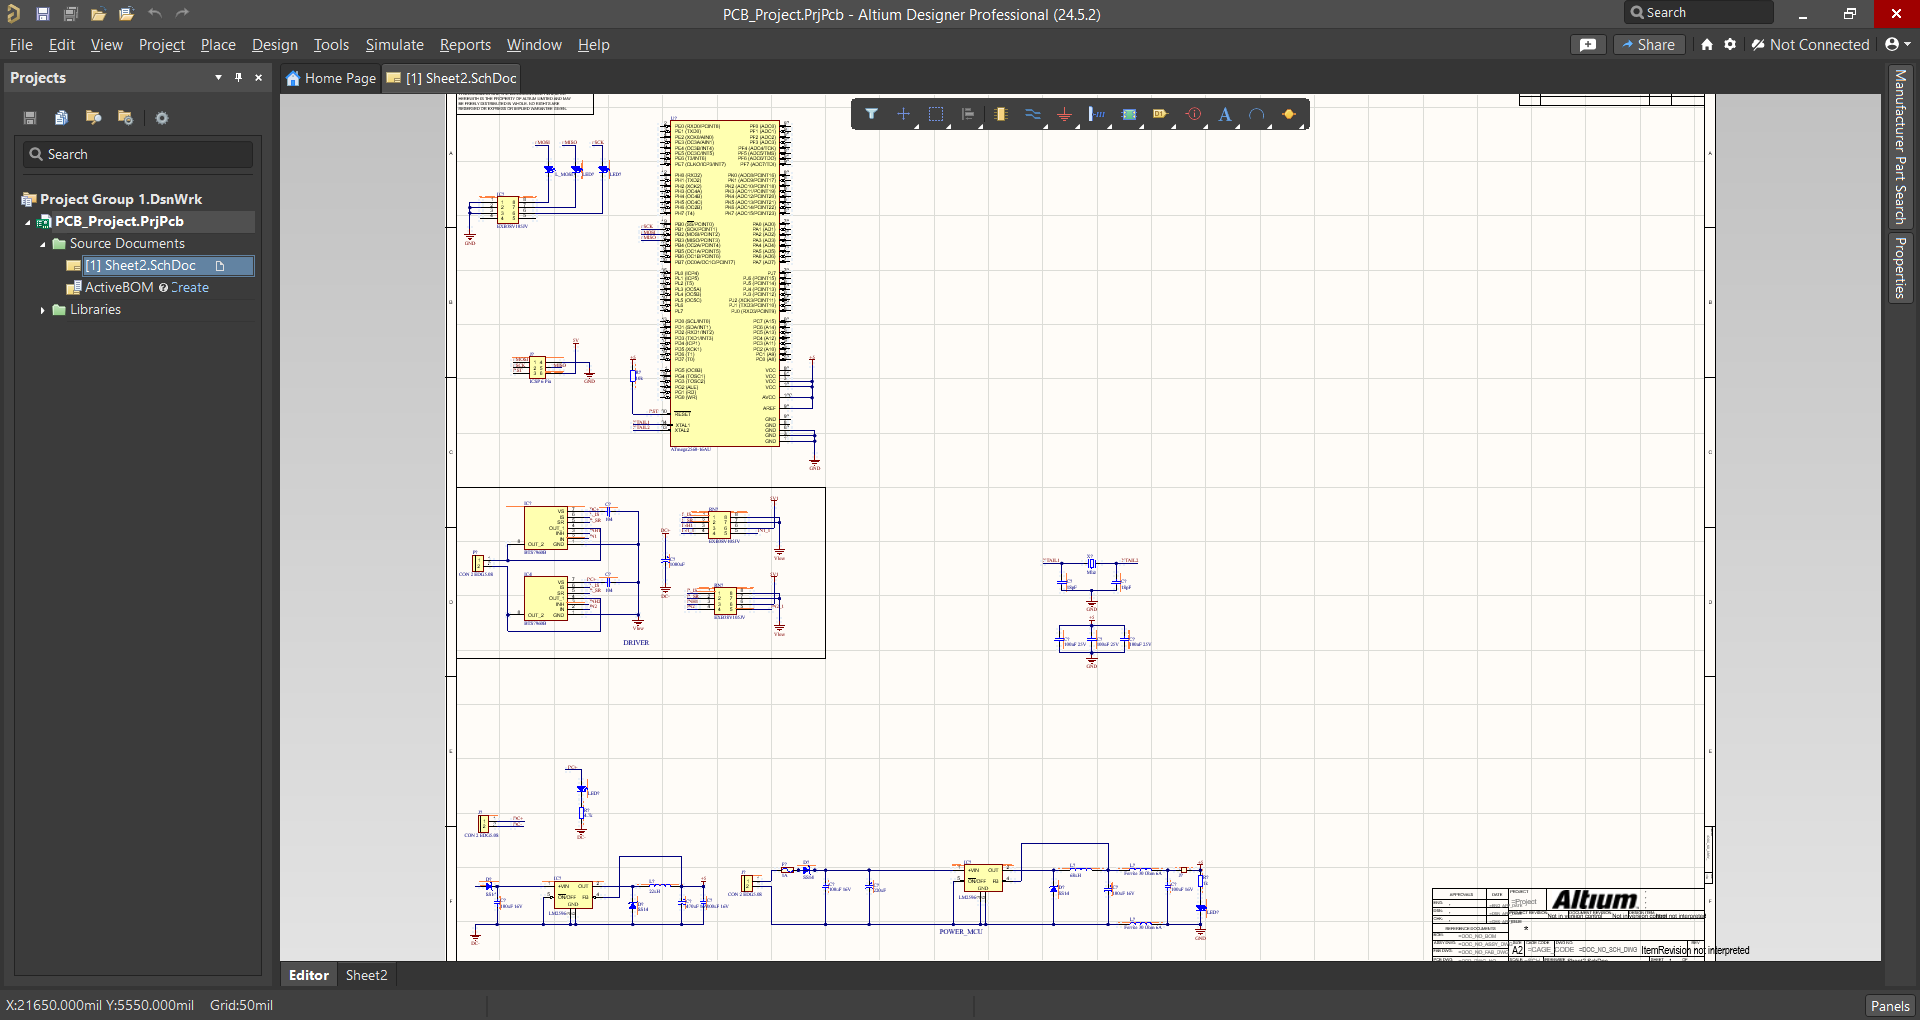
\includegraphics[width=1\textwidth]{pictures/workspacealtium.png}
            \caption{Giao diện làm việc của phần mềm Altium Designer}
            \label{fig:workspacealtium}
        \end{figure}
        \cleardoublepage
    \section{Sơ đồ nguyên lý}
        \subsection{Sơ lược về sơ đồ nguyên lý}
            Sơ đồ nguyên lý trong mạch điện tử là một biểu đồ biểu diễn các thành phần của
            mạch điện và cách chúng được kết nối với nhau. Mục tiêu là để mô tả chức năng của
            mạch một cách rõ ràng và dễ hiểu. Các thành phần phổ biến trong sơ đồ nguyên lý của
            mạch điện tử bao gồm:
            \begin{itemize}
                \item Điện trở (Resistor): Ký hiệu bằng hình chữ nhật hoặc zigzag. Điện trở được sử dụng để giới hạn dòng điện hoặc phân chia điện áp.
                \item Tụ điện (Capacitor): Ký hiệu bằng hai đường thẳng song song. Tụ điện lưu trữ và phóng điện năng.
                \item Cuộn cảm (Inductor): Ký hiệu bằng một loạt các vòng xoắn. Cuộn cảm lưu trữ năng lượng trong từ trường khi dòng điện chạy qua.
                \item Điốt (Diode): Ký hiệu bằng một tam giác và một vạch đứng. Điốt cho phép dòng điện chạy theo một chiều duy nhất.
                \item Transistor:
                \begin{itemize}
                    \item NPN: Ký hiệu bằng một mũi tên chỉ ra ngoài từ đường nối giữa base và emitter.
                    \item PNP: Ký hiệu bằng một mũi tên chỉ vào trong.
                \end{itemize}
                \item IC (Integrated Circuit): Ký hiệu bằng một hình chữ nhật với nhiều chân ra. IC chứa nhiều linh kiện điện tử tích hợp bên trong.
                \item Nguồn điện (Power Supply): Ký hiệu bằng hai đường thẳng song song, với một đường dài hơn (dương) và một đường ngắn hơn (âm).
            \end{itemize}
        \subsection{Ví dụ về sơ đồ nguyên lý}
            \begin{figure}[H]
                \centering
                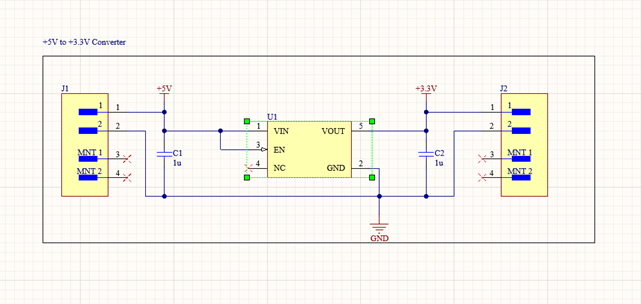
\includegraphics[width=1\textwidth]{pictures/sch1.png}
                \caption{Sơ đồ nguyên lý mạch chuyển đổi điện áp}
                \label{fig:sodonguyenly}
            \end{figure}
            \begin{figure}[H]
                \centering
                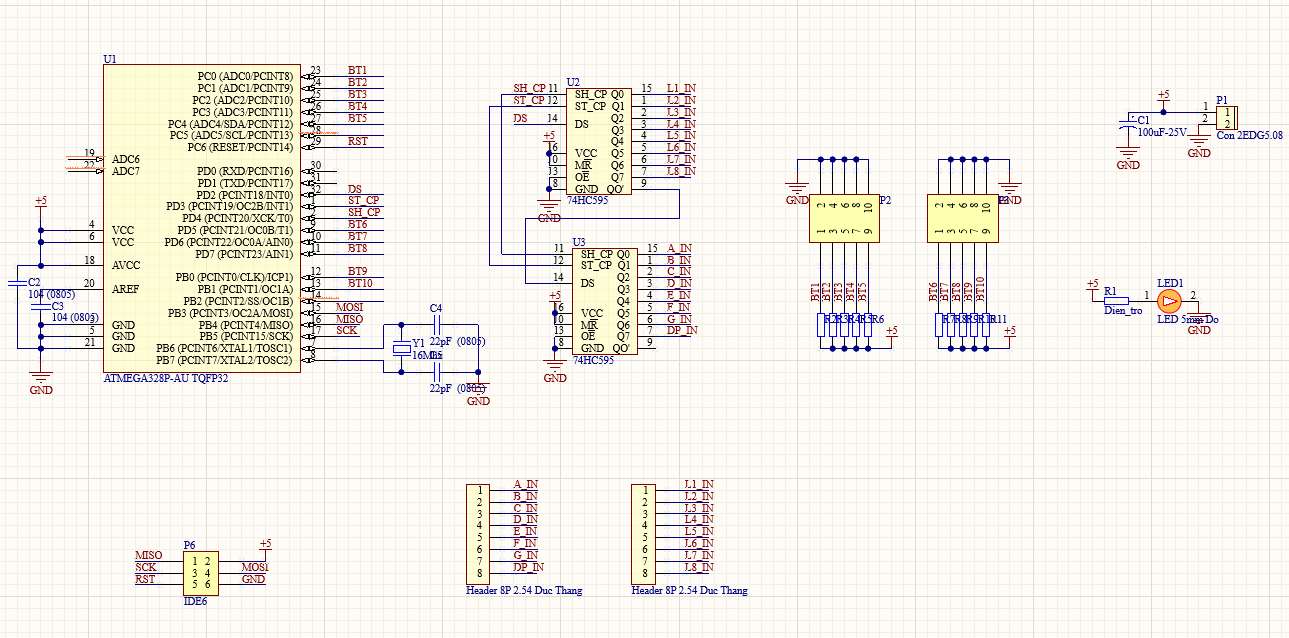
\includegraphics[width=1\textwidth]{pictures/sch2.png}
                \caption{Sơ đồ nguyên lý mạch điều khiển LED 7 đoạn}
                \label{fig:sodonguyenly}
            \end{figure}
            \begin{figure}[H]
                \centering
                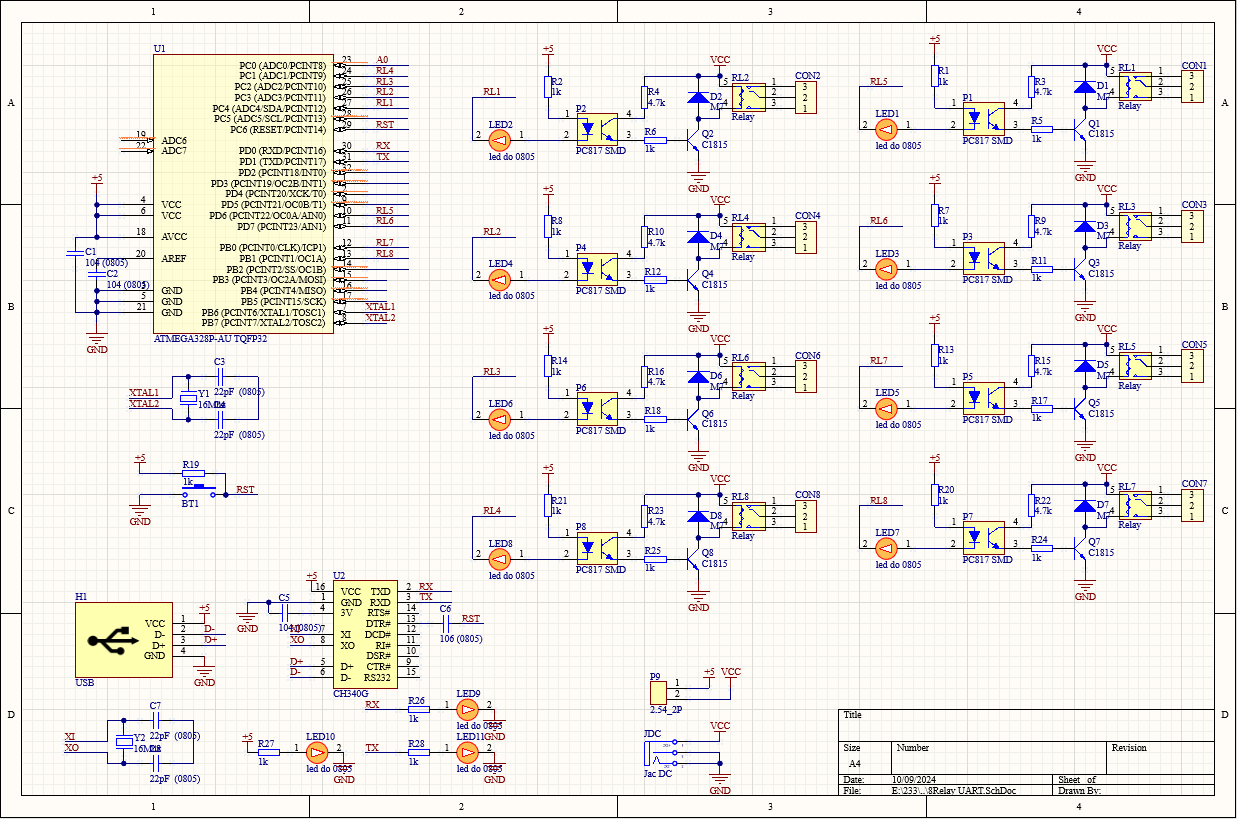
\includegraphics[width=1\textwidth]{pictures/sch3.png}
                \caption{Sơ đồ nguyên lý mạch điều khiển 8 relay}
                \label{fig:sodonguyenly}
            \end{figure}
            \begin{figure}[H]
                \centering
                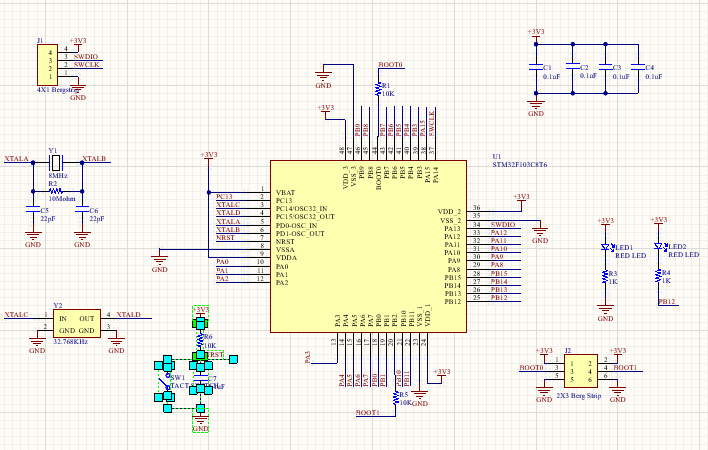
\includegraphics[width=1\textwidth]{pictures/sch4a.png}
                \caption{Sơ đồ nguyên lý mạch STM32F103C8T6 phần điều khiển}
                \label{fig:sodonguyenly}
            \end{figure}
            \begin{figure}[H]
                \centering
                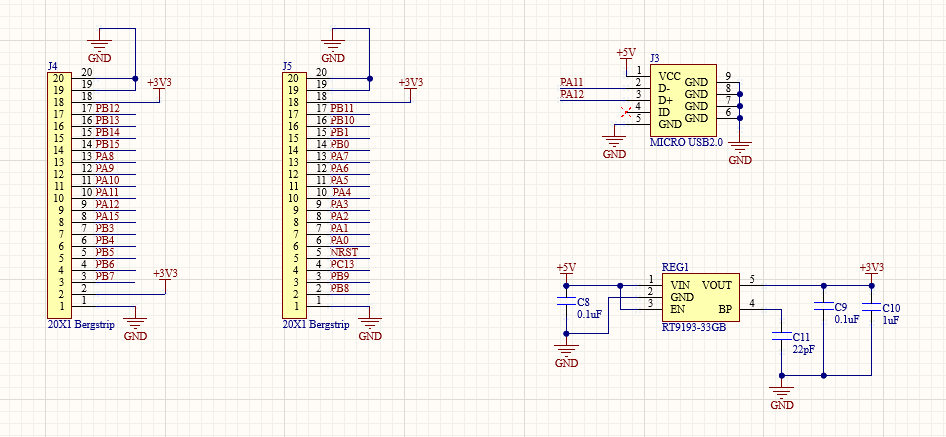
\includegraphics[width=1\textwidth]{pictures/4b.png}
                \caption{Sơ đồ nguyên lý mạch STM32F103C8T6 phần kết nối}
                \label{fig:sodonguyenly}
            \end{figure}
            \begin{figure}[H]
                \centering
                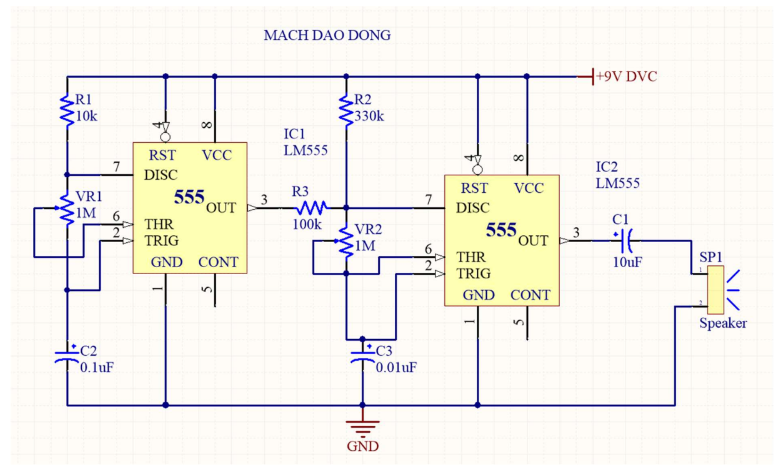
\includegraphics[width=1\textwidth]{pictures/sch5.png}
                \caption{Sơ đồ nguyên lý mạch dao động}
                \label{fig:sodonguyenly}
            \end{figure}
            \cleardoublepage
    \section{Mạch in PCB}
        \subsection{Sơ lược về mạch in PCB}
            Sơ đồ mạch in (PCB - Printed Circuit Board) là một bản vẽ chi tiết mô tả các
            thành phần và kết nối điện tử trên một bảng mạch. Để thiết kế một sơ đồ mạch in PCB,
            bạn cần phải thực hiện các bước cơ bản sau: 
            \begin{itemize}
                \item Xác định yêu cầu:
                \begin{itemize}
                    \item Xác định các thành phần cần thiết cho mạch.
                    \item Định rõ các yêu cầu về điện áp, dòng điện, và tần số.
                \end{itemize}
                \item Thiết kế sơ đồ nguyên lý (schematic):
                \begin{itemize}
                    \item Vẽ sơ đồ nguyên lý để biểu diễn các thành phần điện tử và kết nối giữa chúng.
                    \item Sử dụng phần mềm thiết kế mạch điện tử như Eagle, KiCad, Altium Designer,...
                \end{itemize}
                \item Chuyển sơ đồ nguyên lý thành sơ đồ mạch in (PCB layout):
                \begin{itemize}
                    \item Sử dụng phần mềm thiết kế PCB để tạo ra bố trí mạch in từ sơ đồ nguyên lý.
                    \item Đặt các thành phần trên bảng mạch sao cho tối ưu hóa không gian và đảm bảo hiệu quả kết nối điện.
                \end{itemize}
                \item Route các đường mạch:
                \begin{itemize}
                    \item Kết nối các chân của các thành phần bằng các đường mạch trên bảng PCB.
                    \item Đảm bảo các đường mạch không bị chồng chéo và tuân theo quy tắc thiết kế.
                \end{itemize}
                \item Kiểm tra và xác nhận thiết kế:
                \begin{itemize}
                    \item Kiểm tra sơ đồ mạch in để đảm bảo không có lỗi.
                    \item Sử dụng các công cụ kiểm tra DRC (Design Rule Check) để đảm bảo tuân thủ các quy tắc thiết kế.
                \end{itemize}
                \item Xuất file Gerber:
                \begin{itemize}
                    \item Xuất các file Gerber từ phần mềm thiết kế PCB để gửi đến nhà sản xuất PCB.
                    \item File Gerber là định dạng tiêu chuẩn được sử dụng trong sản xuất PCB.
                \end{itemize}
                \item Sản xuất PCB:
                \begin{itemize}
                    \item Gửi các file Gerber đến nhà sản xuất PCB để họ tạo ra bảng mạch thực tế.
                    \item Sau khi sản xuất, kiểm tra bảng mạch để đảm bảo chất lượng.
                \end{itemize}
            \end{itemize}
        \subsection{Ví dụ về mạch in PCB}
            \begin{figure}[H]
                \centering
                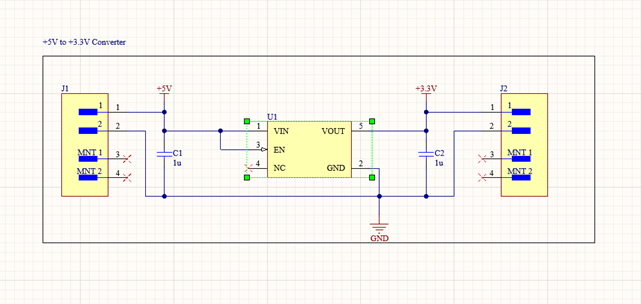
\includegraphics[width=1\textwidth]{pictures/sch1.png}
                \caption{Sơ đồ nguyên lý mạch chuyển đổi điện áp}
                \label{fig:sodonguyenly}
            \end{figure}
            \begin{figure}[H]
                \centering
                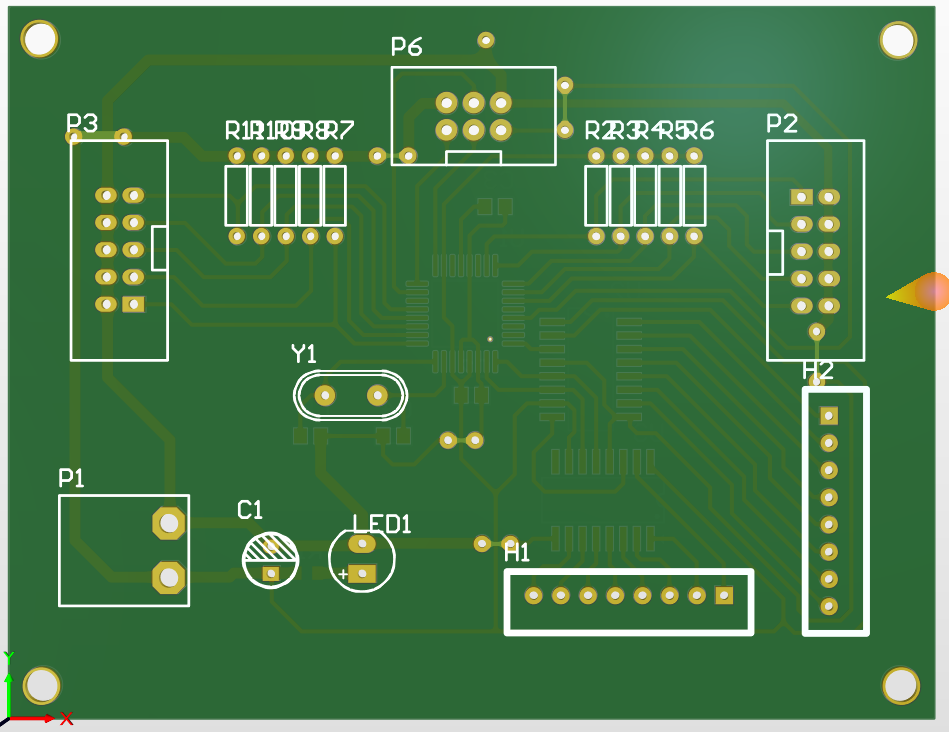
\includegraphics[width=1\textwidth]{pictures/pcb1.png}
                \caption{Mặt trước mạch điều khiển LED 7 đoạn}
                \label{fig:hbridge}
            \end{figure}
            \begin{figure}[H]
                \centering
                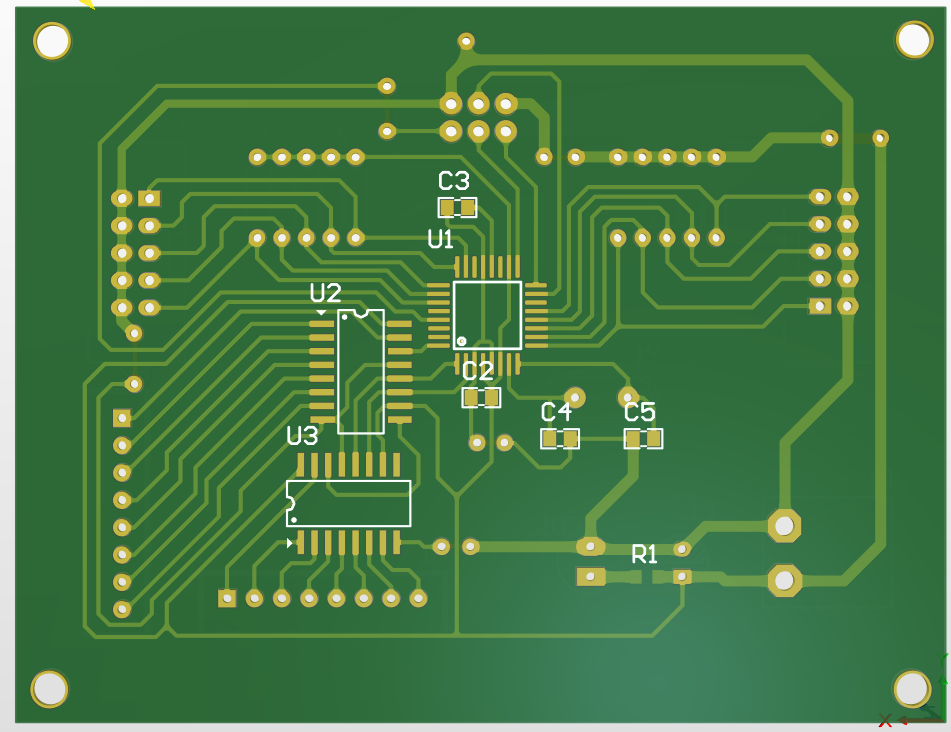
\includegraphics[width=1\textwidth]{pictures/pcb2.png}
                \caption{Mặt sau mạch điều khiển LED 7 đoạn}
                \label{fig:hbridge}
            \end{figure}
            \begin{figure}[H]
                \centering
                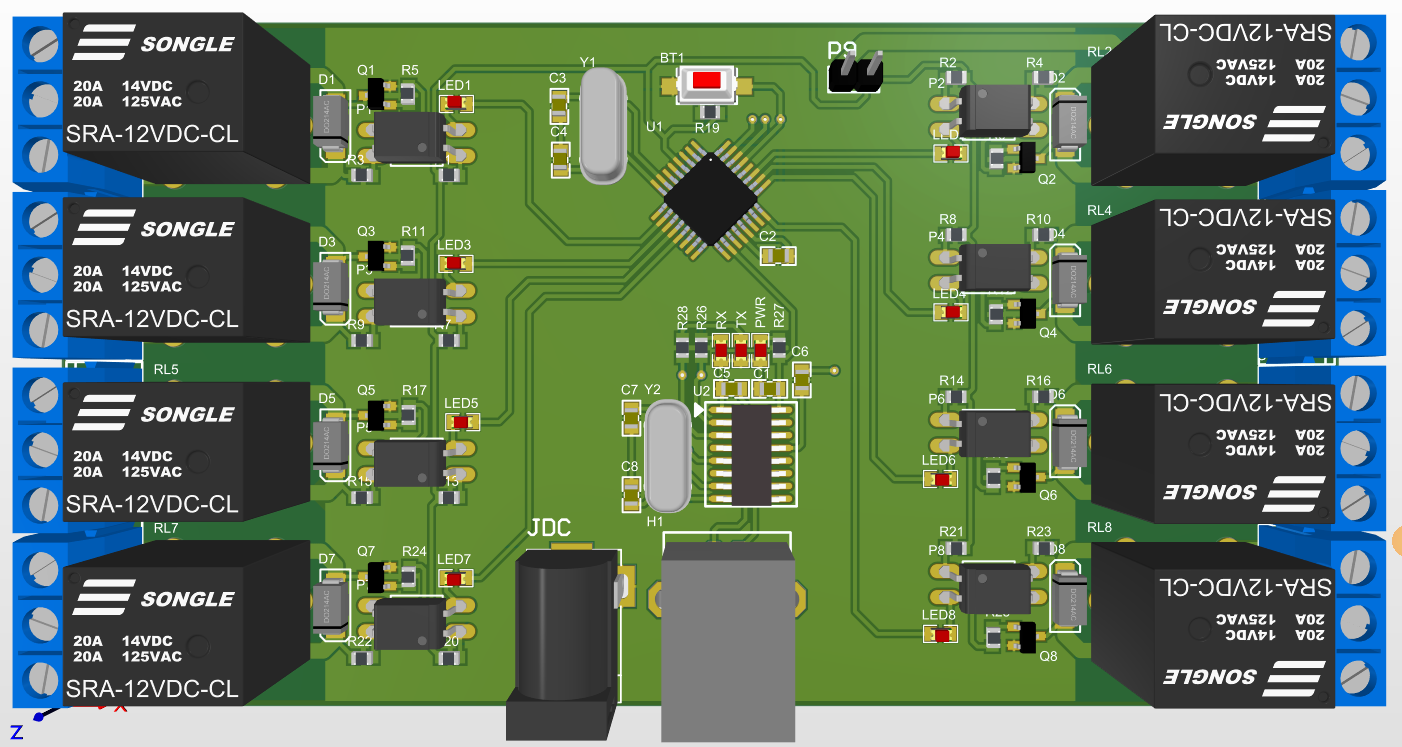
\includegraphics[width=1\textwidth]{pictures/pcb3.png}
                \caption{Mạch điều khiển 8 relay}
                \label{fig:hbridge}
            \end{figure}
            \begin{figure}[H]
                \centering
                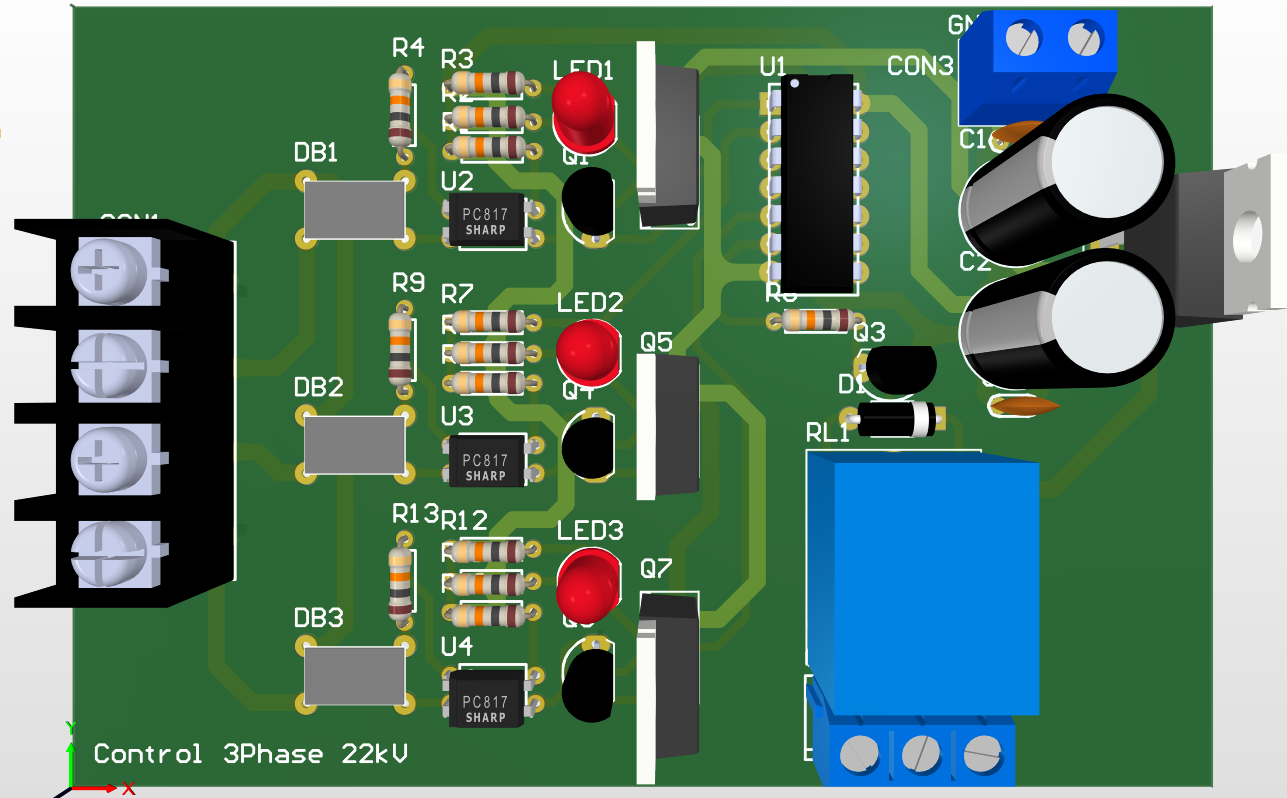
\includegraphics[width=1\textwidth]{pictures/pcb4.png}
                \caption{Mạch điều khiển 3 pha}
                \label{fig:hbridge}
            \end{figure}
            \begin{figure}[H]
                \centering
                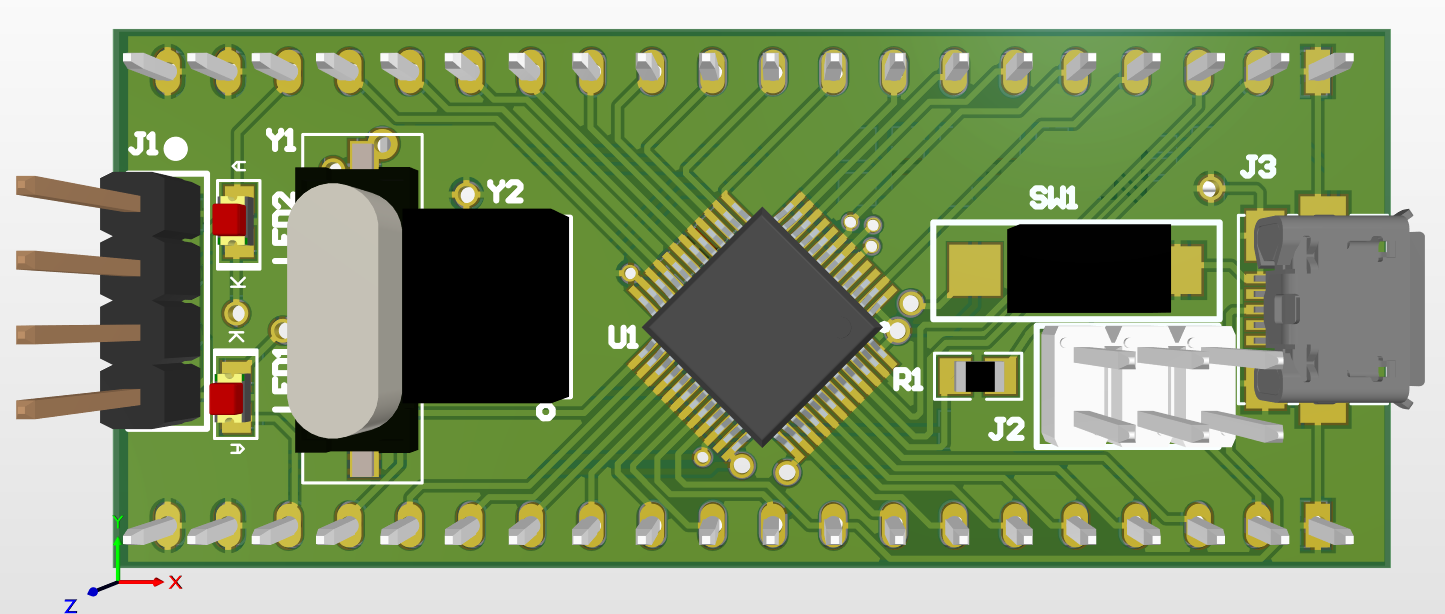
\includegraphics[width=1\textwidth]{pictures/pcb5.png}
                \caption{Mạch STM32F103C8T6}
                \label{fig:hbridge}
            \end{figure}
            \cleardoublepage
        \section{TẠO THƯ VIỆN SCHEMATIC VÀ PCB 3D}
            \subsection{Trình tự tạo thư viện schematic}
                Bước 1: Chọn File/New/Library để tạo thư viện mới.
                \begin{figure}[H]
                    \centering
                    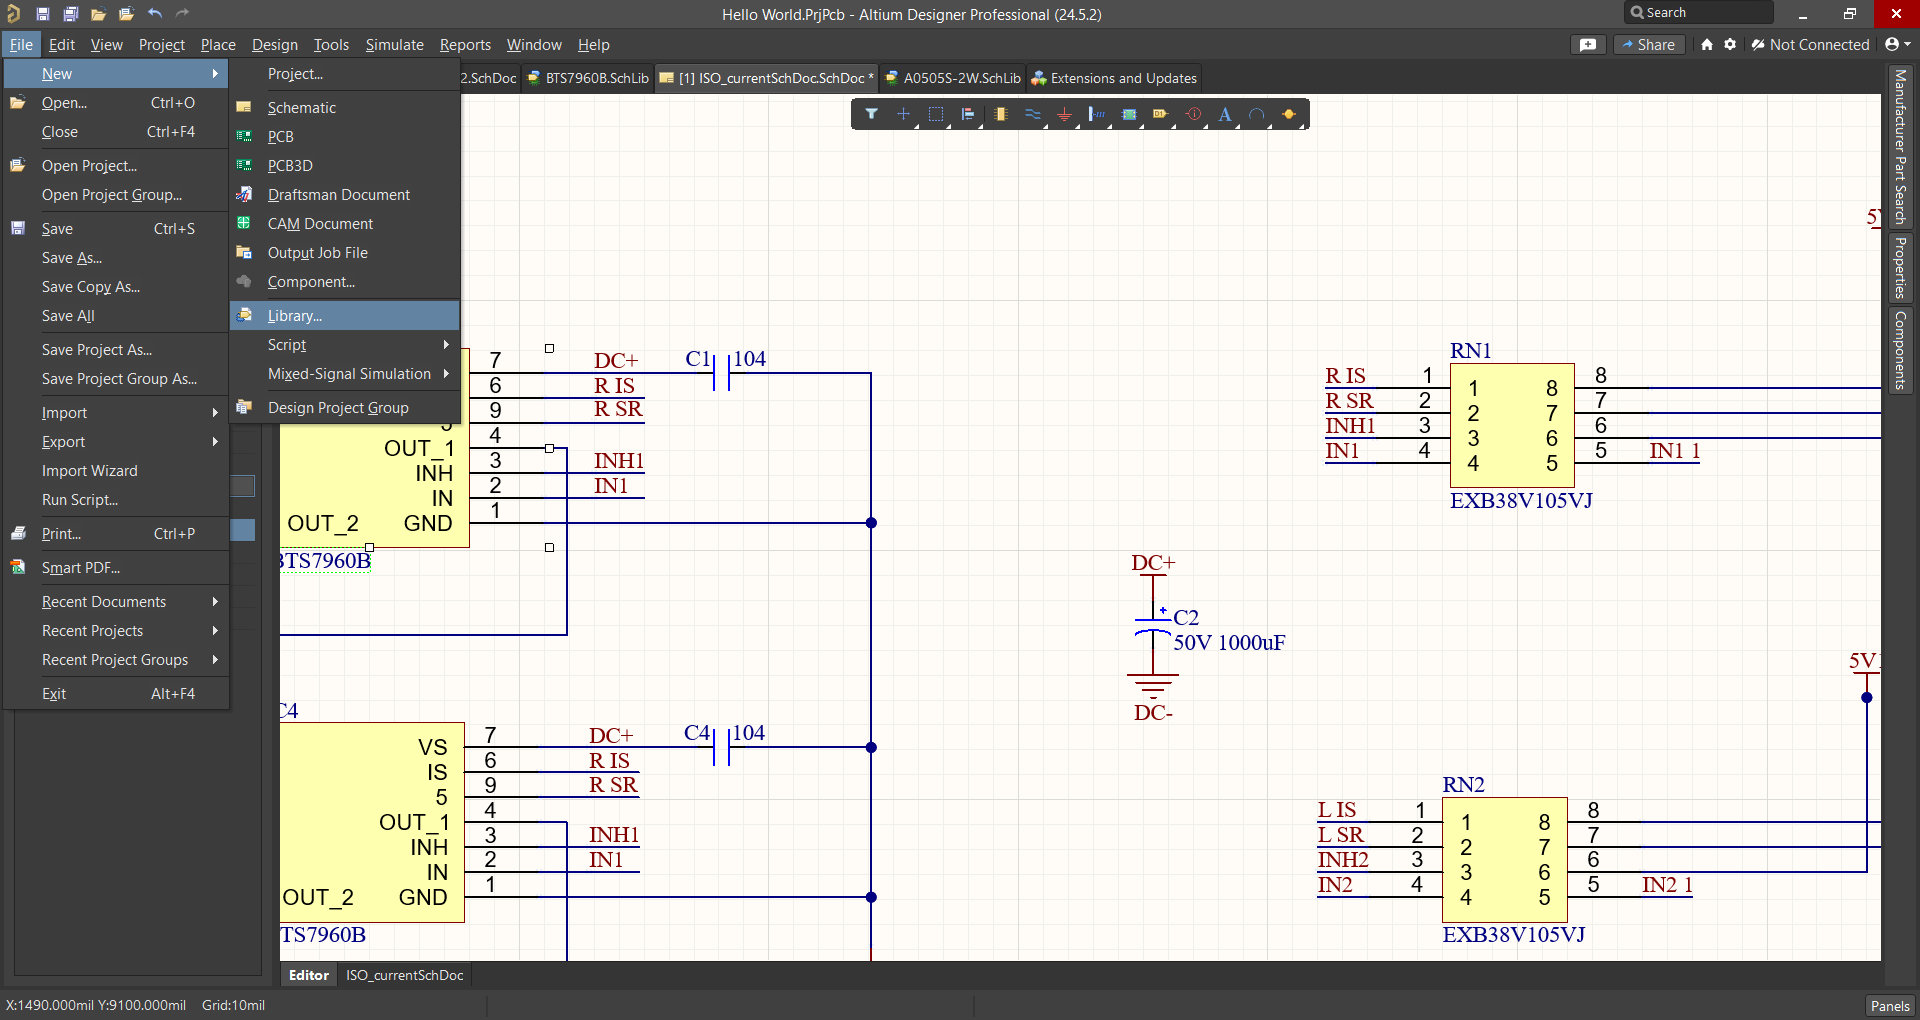
\includegraphics[width=1\textwidth]{pictures/ch3.1.png}
                \end{figure}
                Bước 2: Chọn Schematic Library và nhấn Create.
                \begin{figure}[H]
                    \centering
                    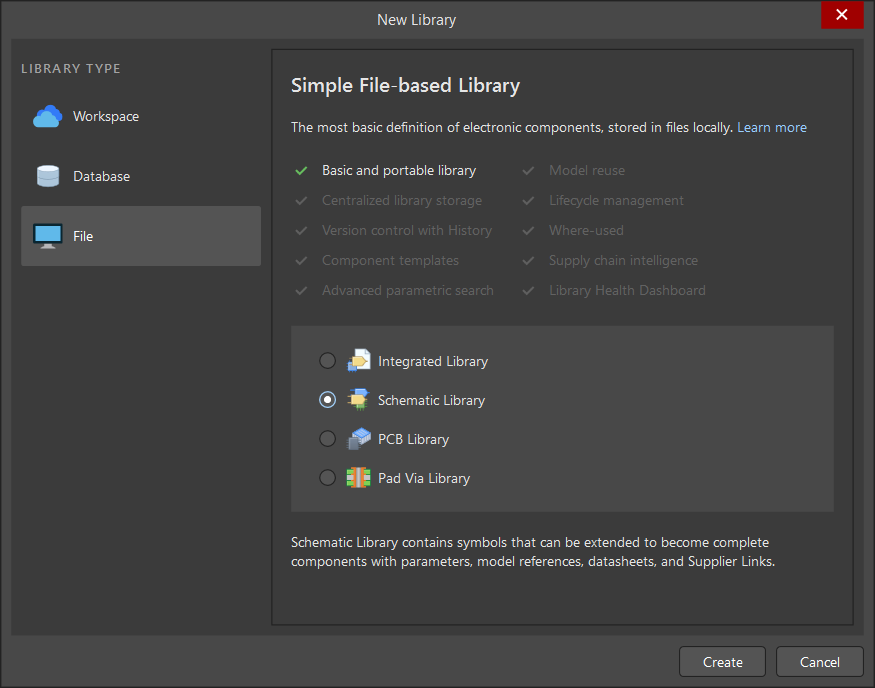
\includegraphics[width=0.8\textwidth]{pictures/ch3.2.png}
                \end{figure}
                Bước 3: Vẽ khối và đặt các chân theo hướng dẫn của datasheet.
                \begin{figure}[H]
                    \centering
                    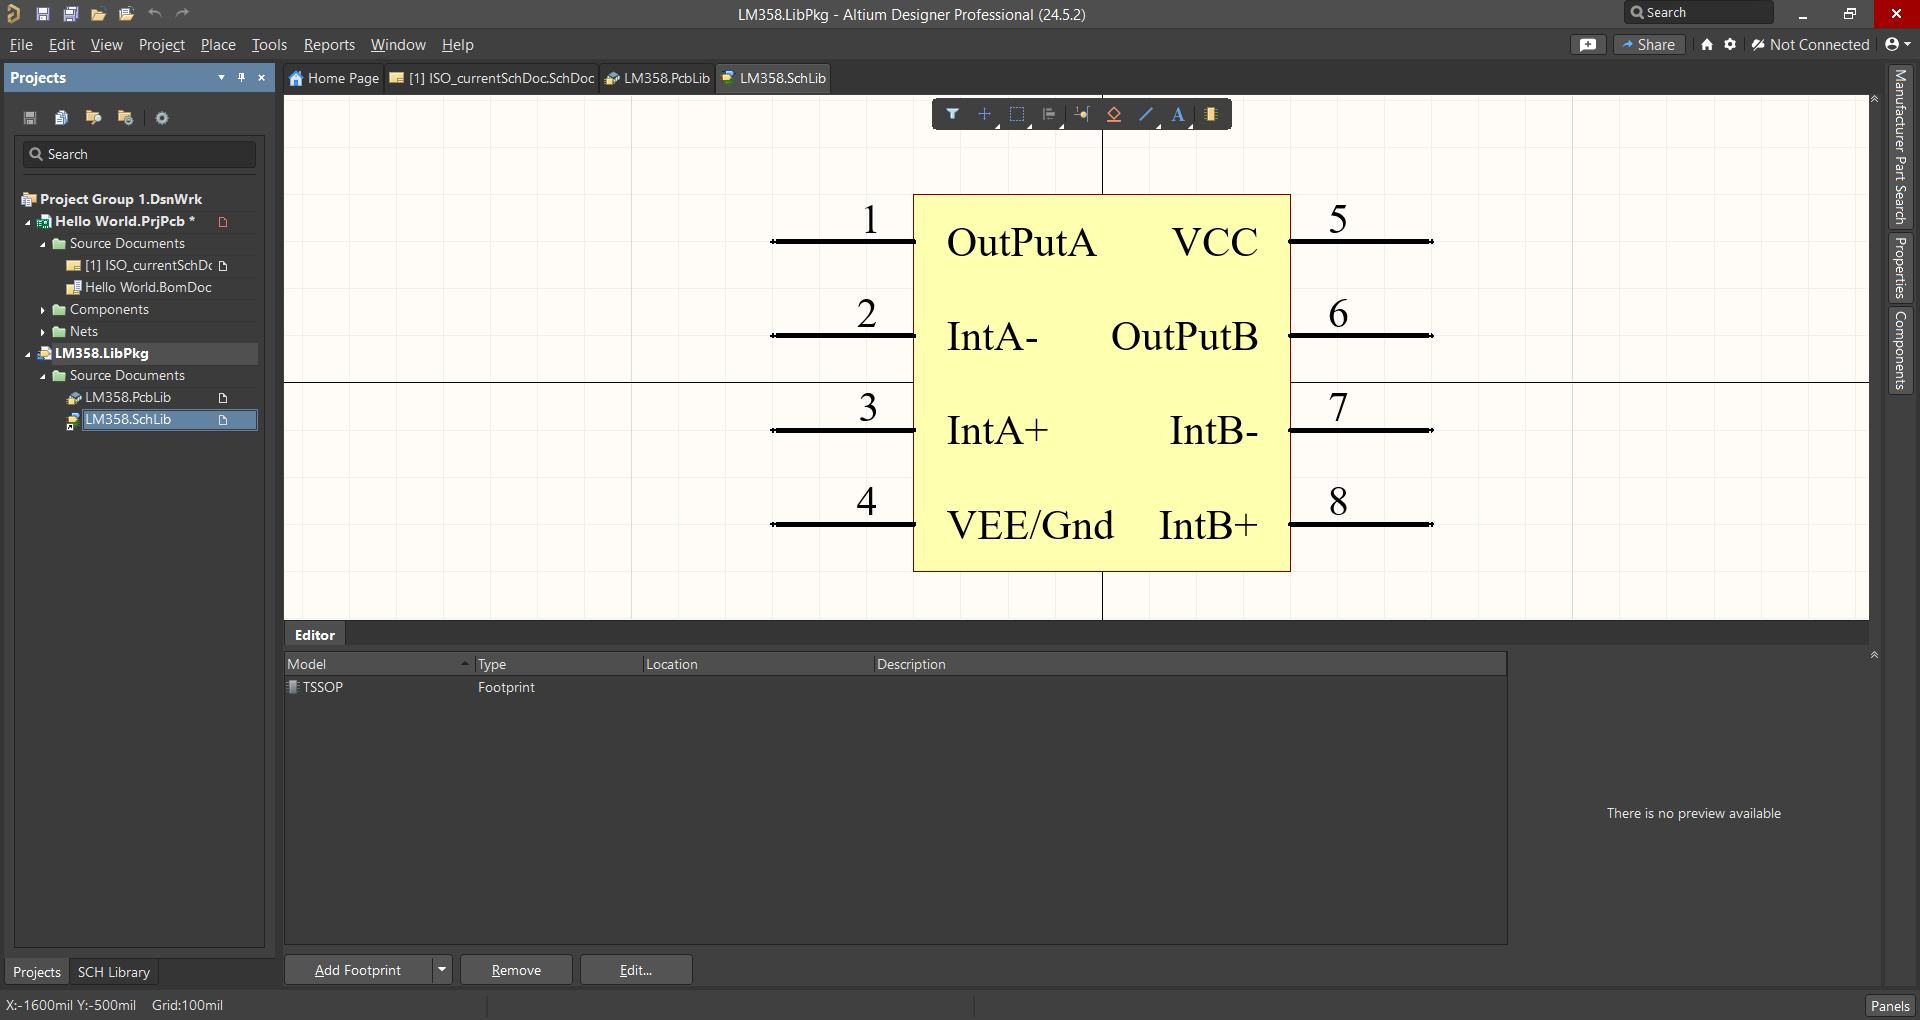
\includegraphics[width=1\textwidth]{pictures/ch3.3.png}
                \end{figure}
                Bước 4: Đặt tên cho thư viện và lưu lại.\\
            \subsection{Trình tự tạo thư viện PCB }
                \textbf{Ví dụ: Tạo thư viện fPCB 3D cho LM358 SOP8.}\\
                Bước 1: Chọn File/New/Library để tạo thư viện mới.\\
                Bước 2: Chọn PCB Library và nhấn Create.
                \begin{figure}[H]
                    \centering
                    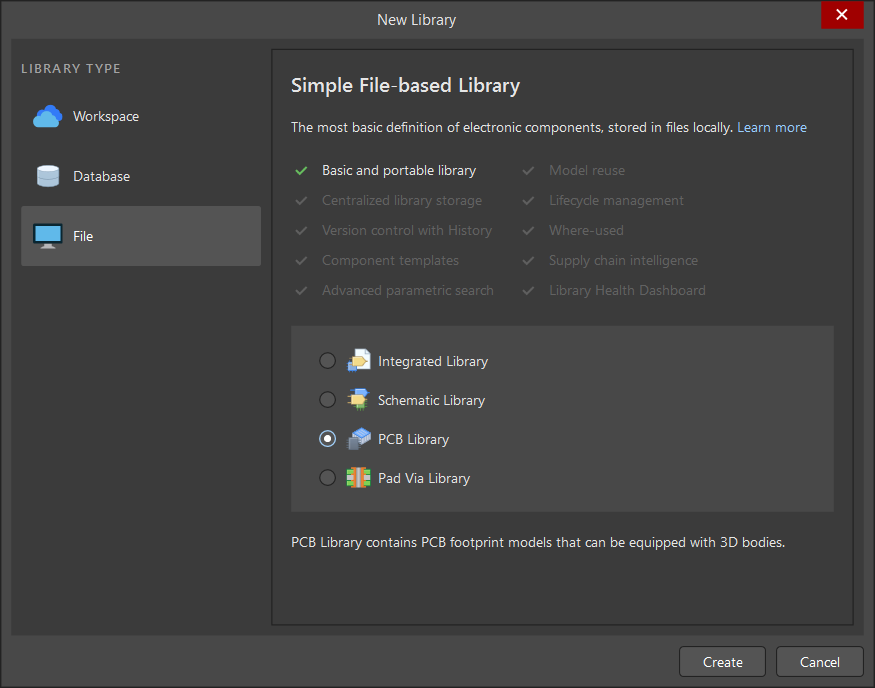
\includegraphics[width=0.7\textwidth]{pictures/ch3.4.png}
                \end{figure}
                Bước 3: Chọn Tools/IPC Compliant Footprint Wizard/Next.
                \begin{figure}[H]
                    \centering
                    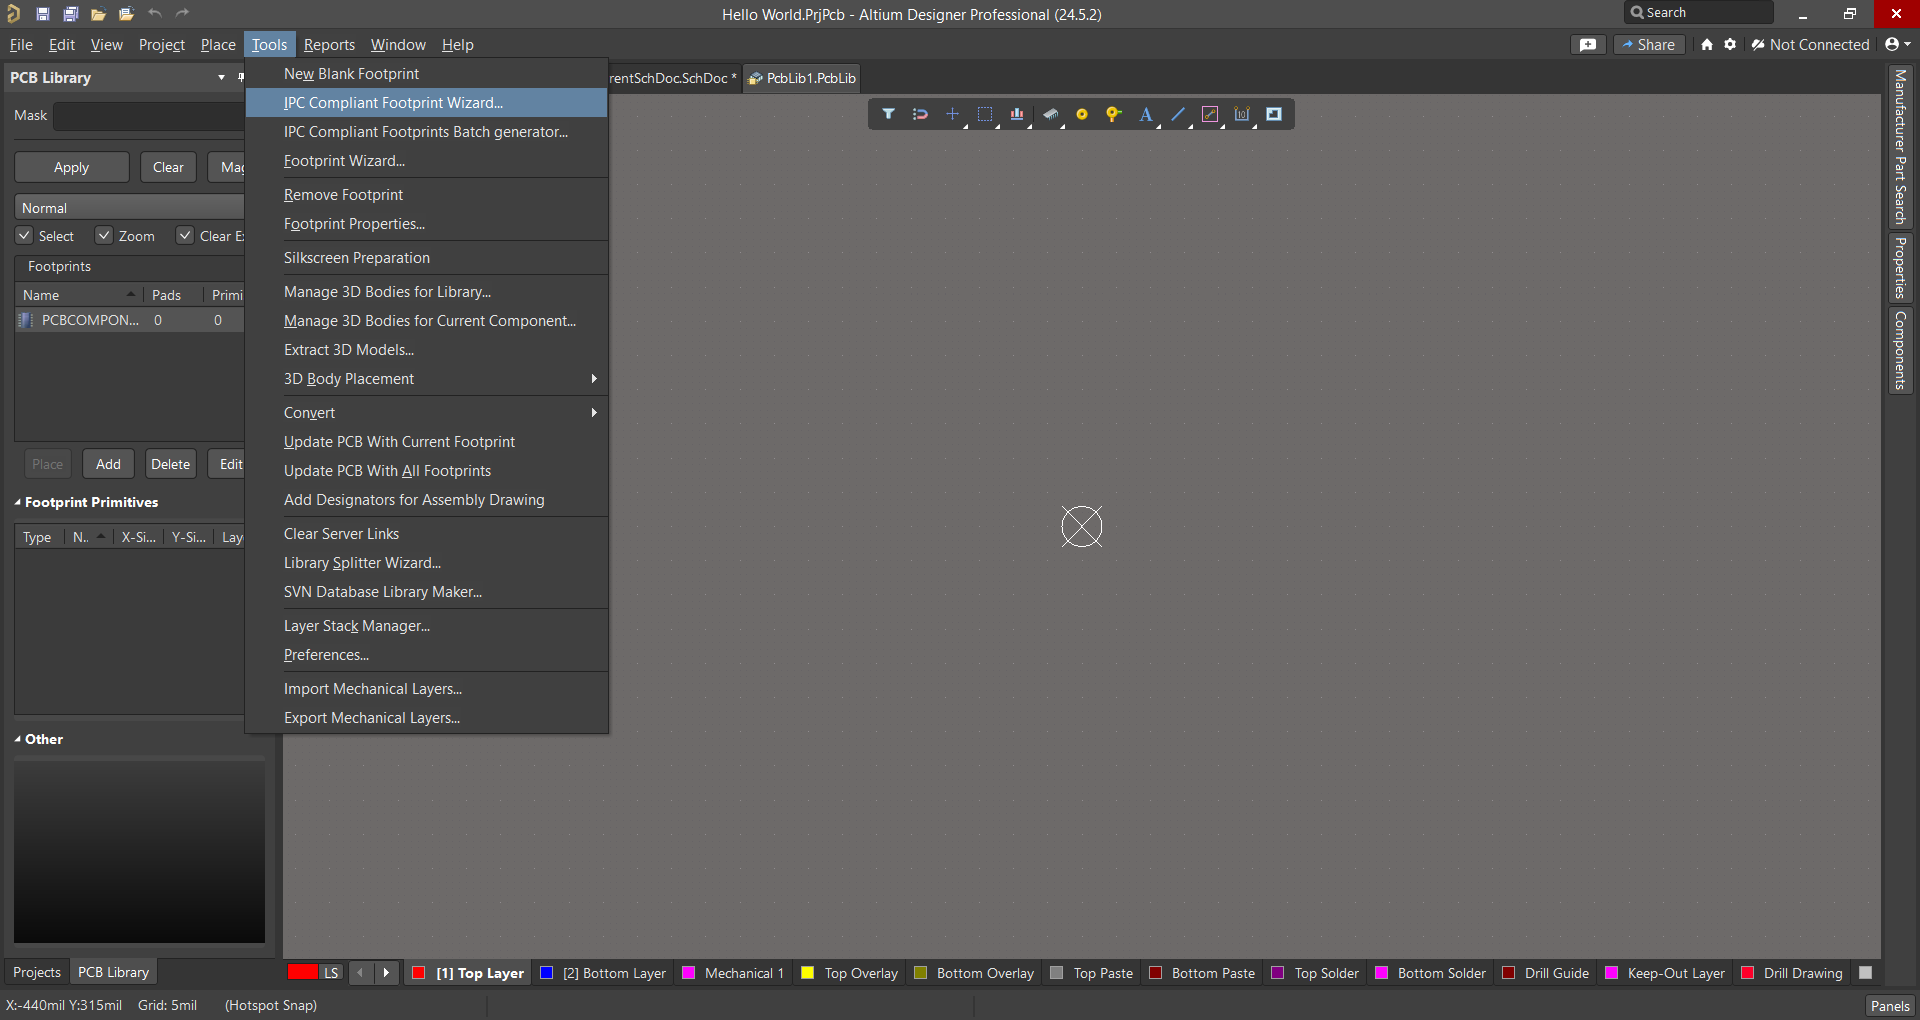
\includegraphics[width=1\textwidth]{pictures/ch3.5.png}
                \end{figure}
                Bước 4: Chọn kiểu chân SOP/TSOP và nhấn NEXT.
                \begin{figure}[H]
                    \centering
                    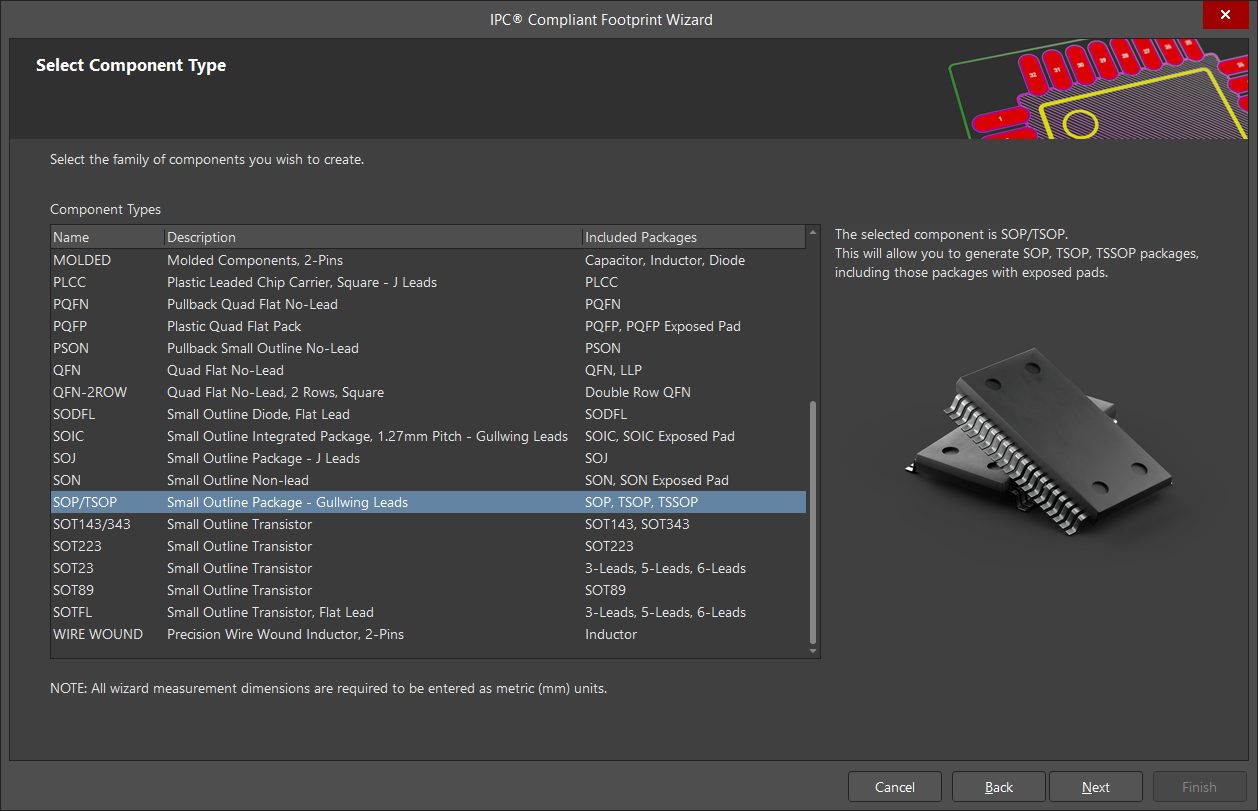
\includegraphics[width=1\textwidth]{pictures/ch3.6.png}
                \end{figure}
                \cleardoublepage
                Bước 5: Đọc datasheet của linh kiện để tìm các thông số thiết kế.
                \begin{figure}[H]
                    \centering
                    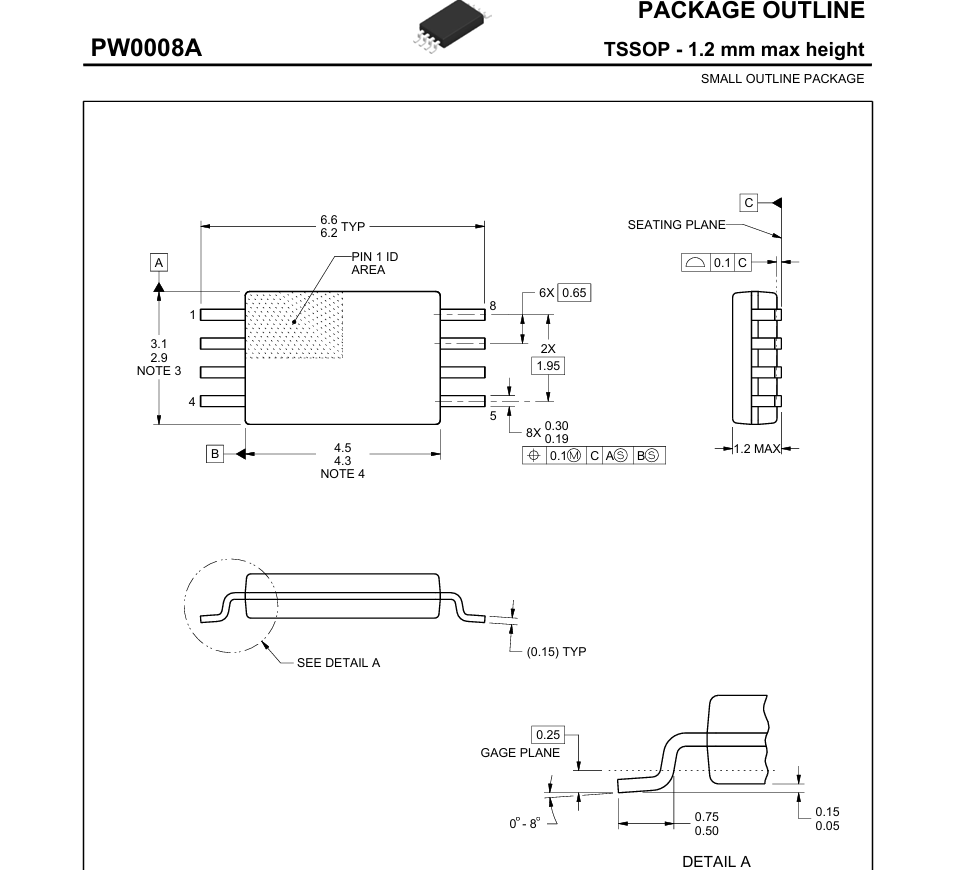
\includegraphics[width=0.9\textwidth]{pictures/ch3.7.png}
                \end{figure}
                Bước 6: Nhập các thông số vào các ô tương ứng và nhấn NEXT.
                \begin{figure}[H]
                    \centering
                    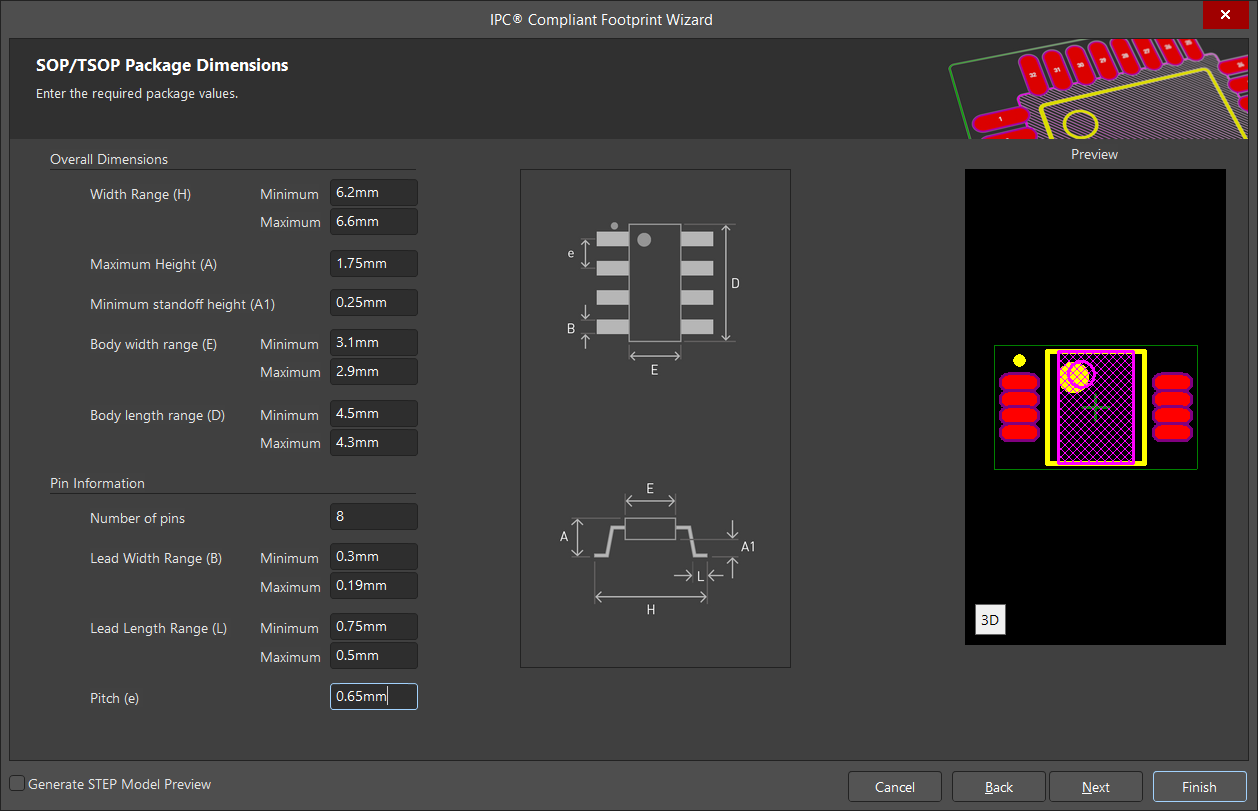
\includegraphics[width=0.8\textwidth]{pictures/ch3.8.png}
                \end{figure}
                Bước 7: Tiếp tục nhấn NEXT cho đến khi đến màn hình lưu và đặt tên.
                \begin{figure}[H]
                    \centering
                    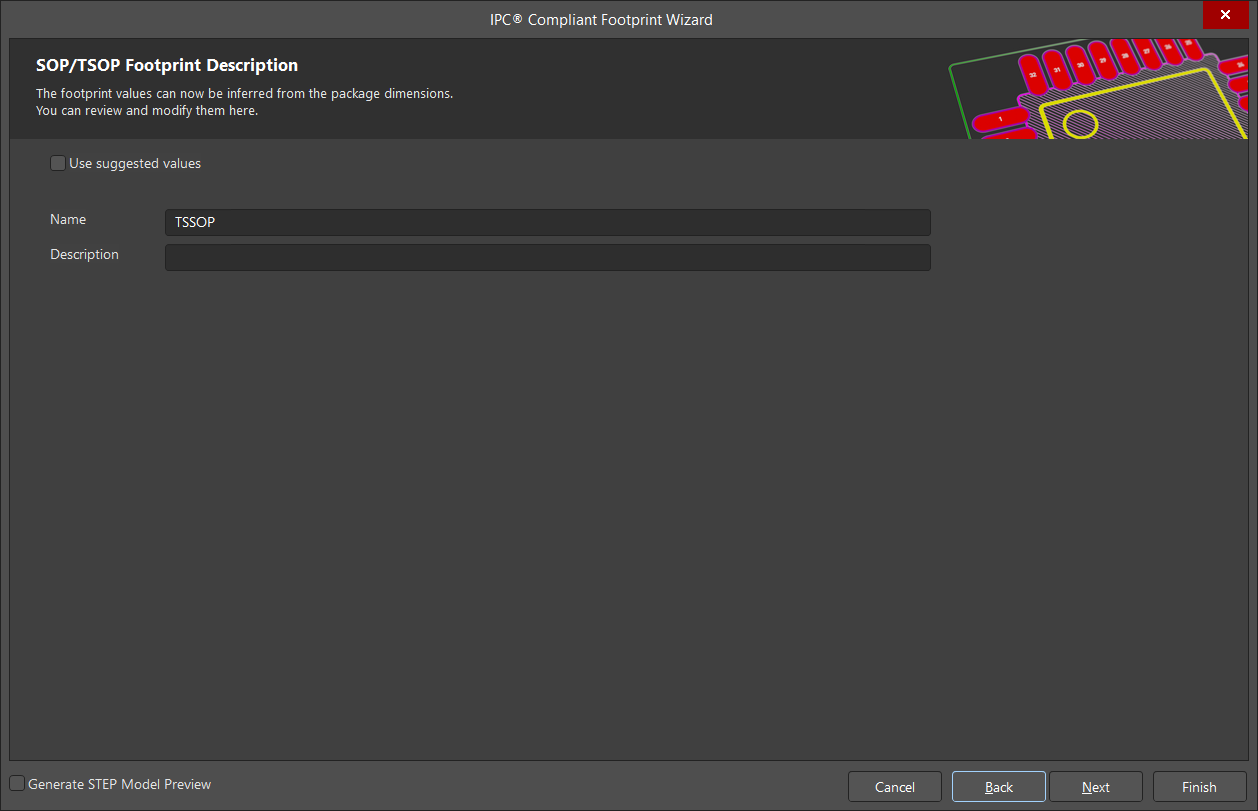
\includegraphics[width=1\textwidth]{pictures/ch3.9.png}
                \end{figure}
                Bước 8: Chọn Produce 3D/STEP model nhấn NEXT và FINISH.
                \begin{figure}[H]
                    \centering
                    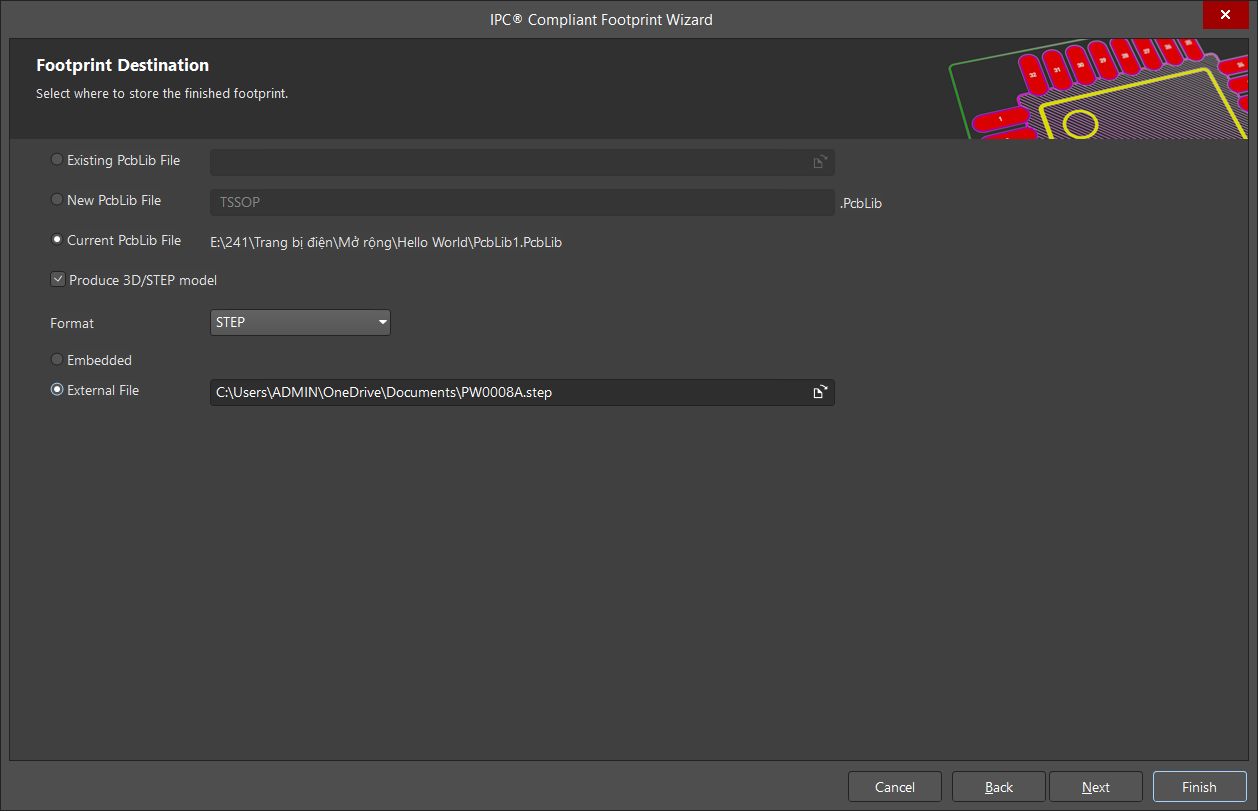
\includegraphics[width=1\textwidth]{pictures/ch3.10.png}
                \end{figure}
                \cleardoublepage
                Bước 9: Hoàn thành việc tạo thư viện footprint cho linh kiện LM358 SOP8.
                \begin{figure}[H]
                    \centering
                    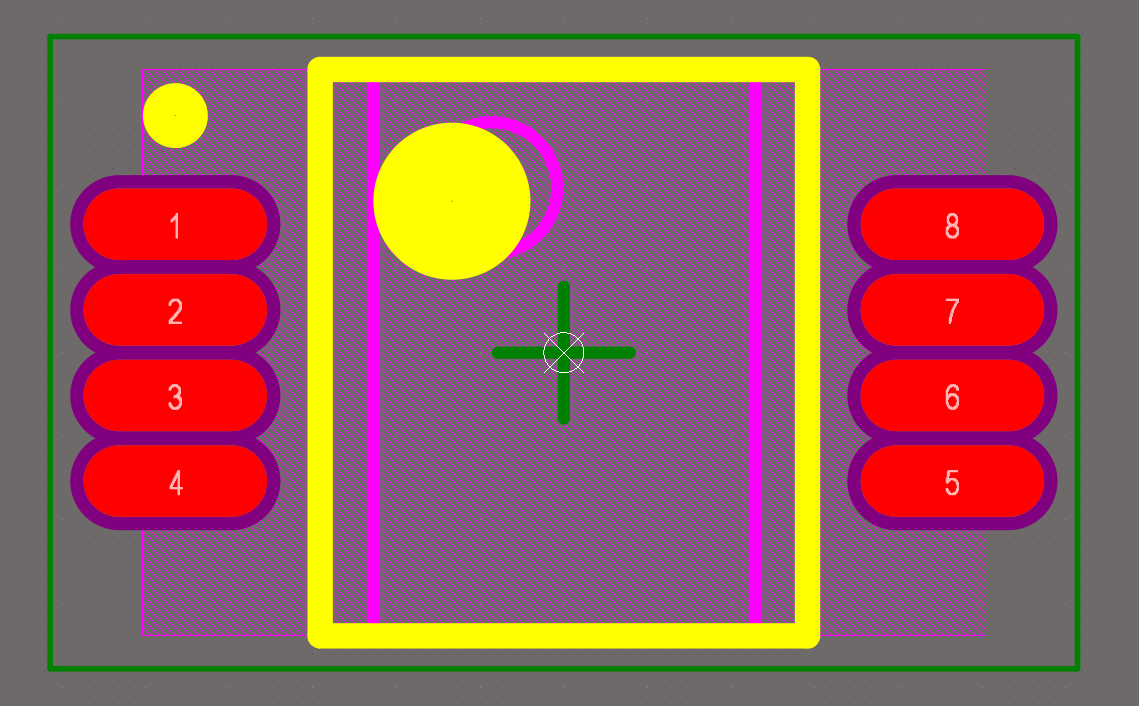
\includegraphics[width=0.9\textwidth]{pictures/ch3.11a.png}
                    \caption{Footprint LM358 SOP8 vừa tạo} 
                \end{figure}
                \begin{figure}[H]
                    \centering
                    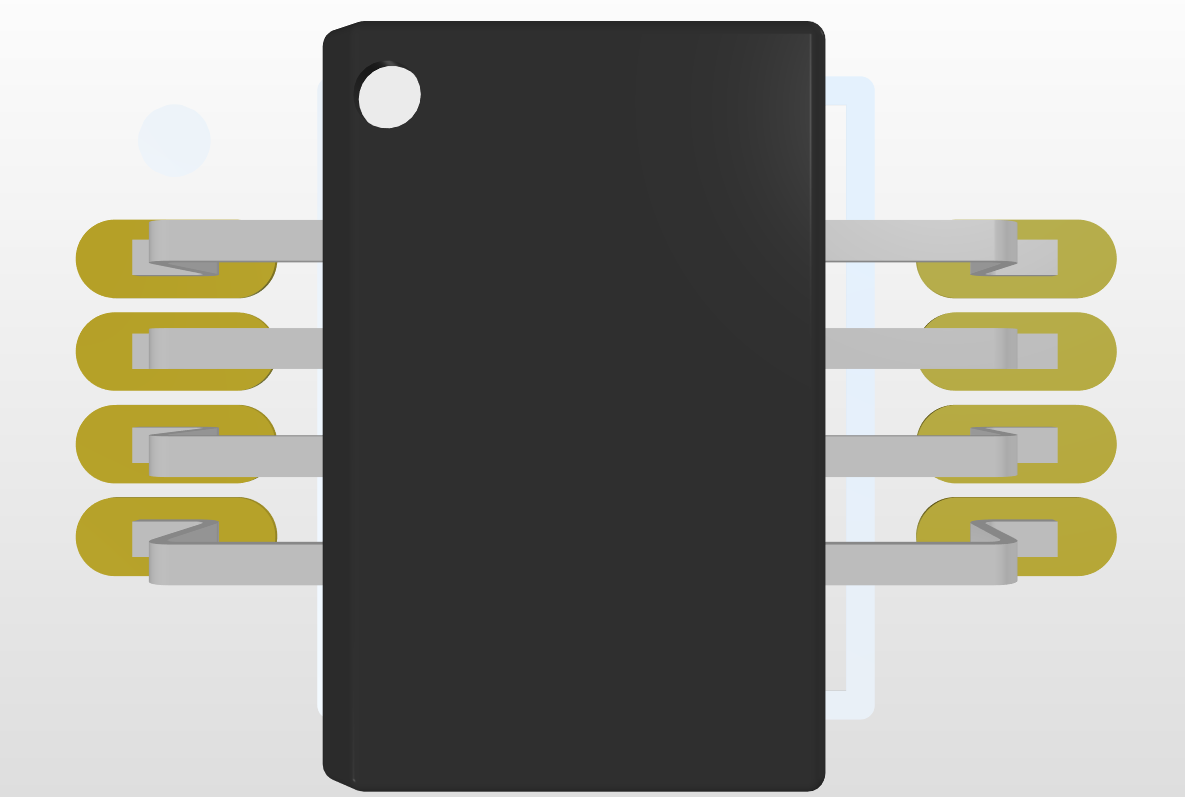
\includegraphics[width=0.9\textwidth]{pictures/ch3.11b.png}
                    \caption{Mô hình PCB 3D LM358 SOP8 vừa tạo}
                \end{figure}
                \cleardoublepage
            \subsection{Add thư viện schematic và thư viện PCB lại với nhau}
                Bước 1: Ở màn hình làm việc của thư viện schematic chọn Add Footprint.
                \begin{figure}[H]
                    \centering
                    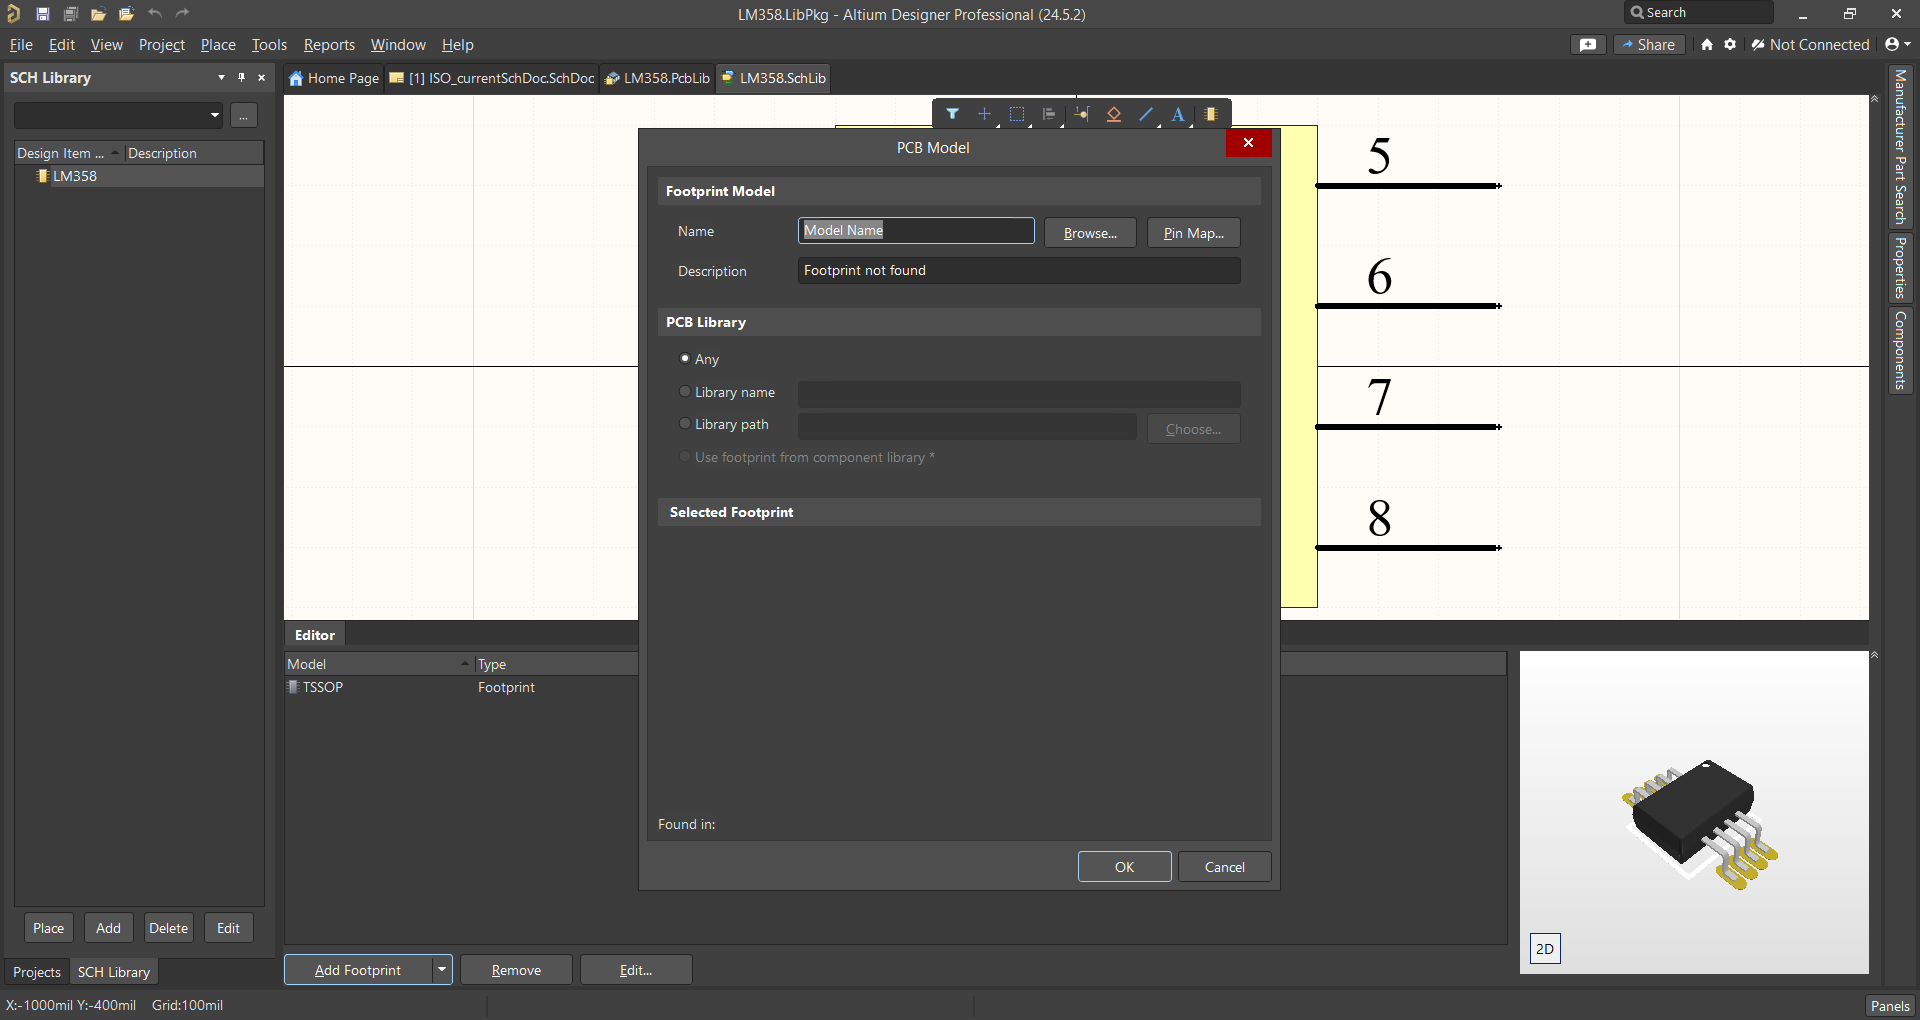
\includegraphics[width=1\textwidth]{pictures/ch3.12.png}
                \end{figure}
                Bước 2: Chọn Browse và chọn thư viện PCB tương ứng và nhấn OK
                \begin{figure}[H]
                    \centering
                    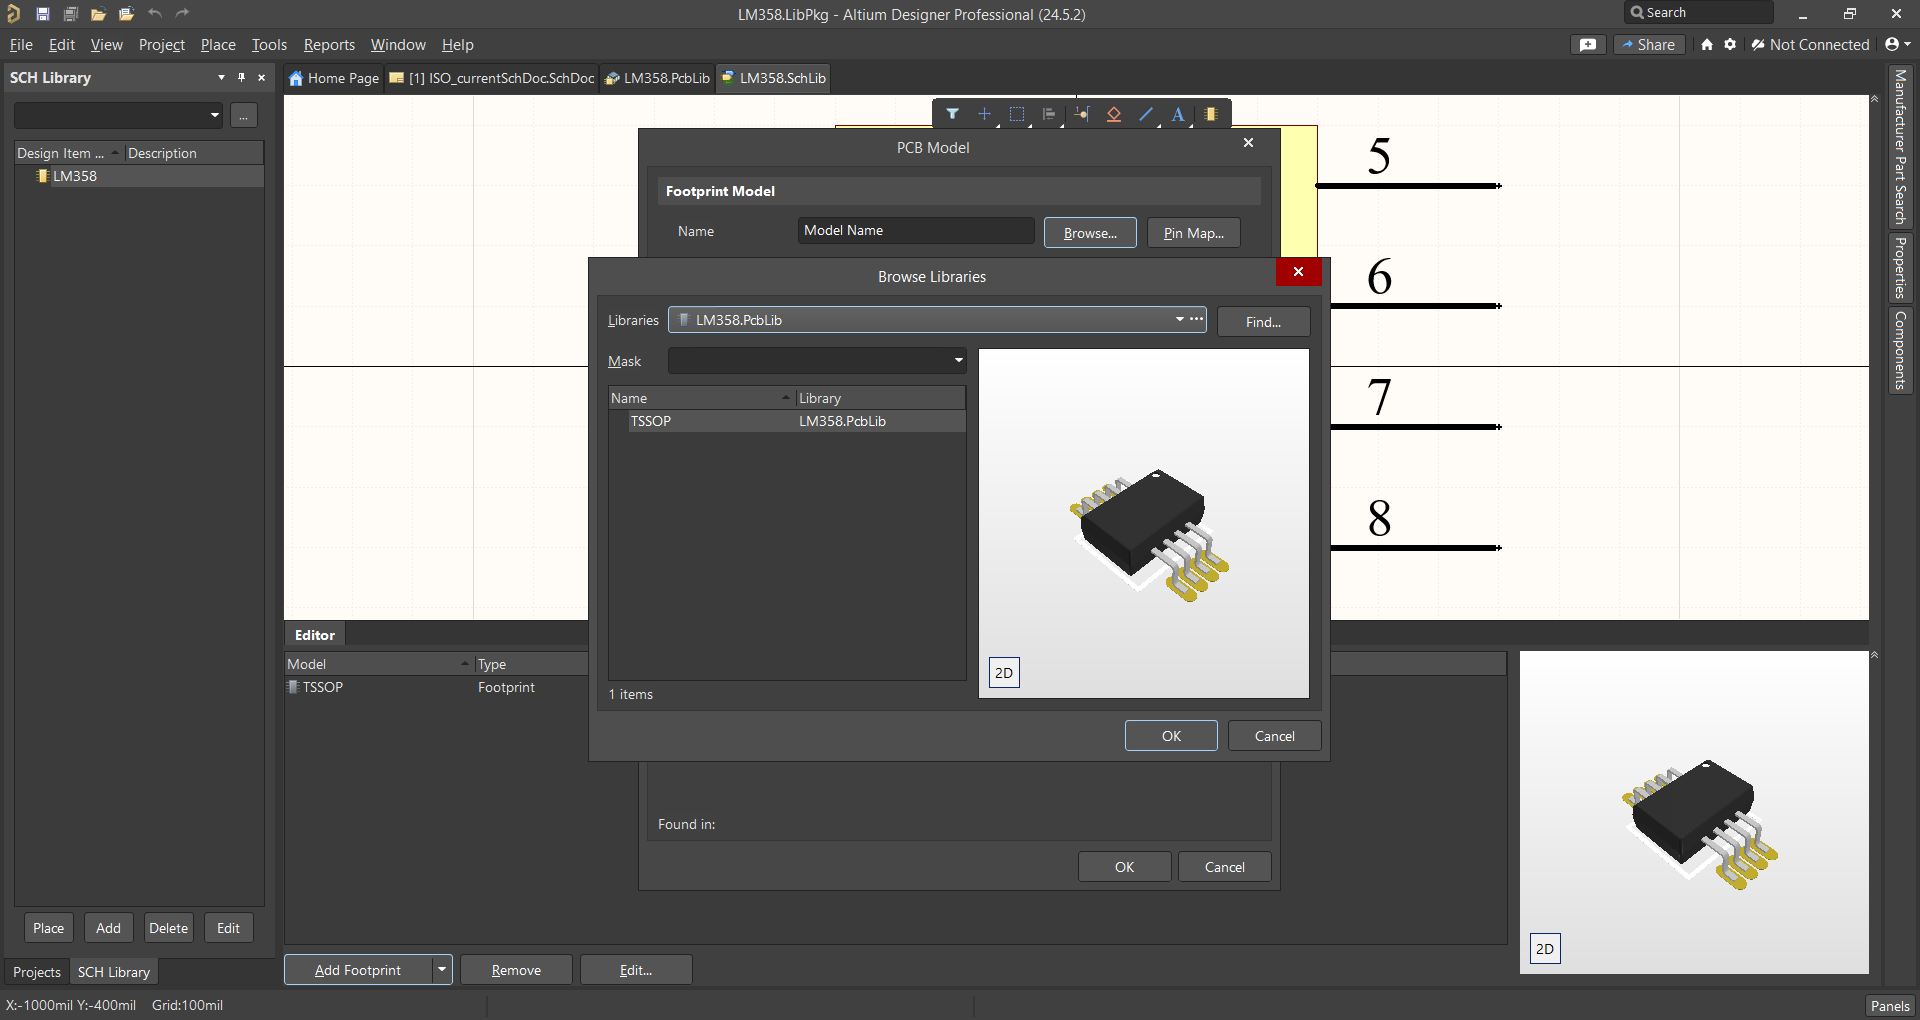
\includegraphics[width=1\textwidth]{pictures/ch3.13.png}
                \end{figure}
                \cleardoublepage
                Bước 3: Vào File/New chọn Library và chọn Integrated Library.
                \begin{figure}[H]
                    \centering
                    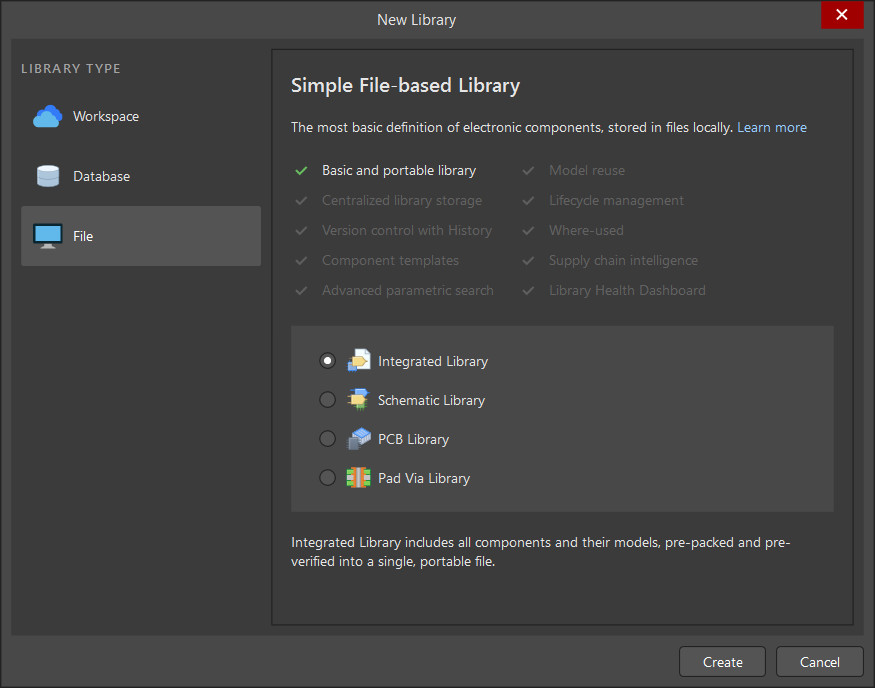
\includegraphics[width=1\textwidth]{pictures/ch3.15.png}
                \end{figure}
                Bước 4: Kéo 2 thư viện schematic và PCB vào Integrated Library vừa tạo và lưu lại. 
                Bước 5: Click chuột phải và chọn Compile Integrated Library.
                \begin{figure}[H]
                    \centering
                    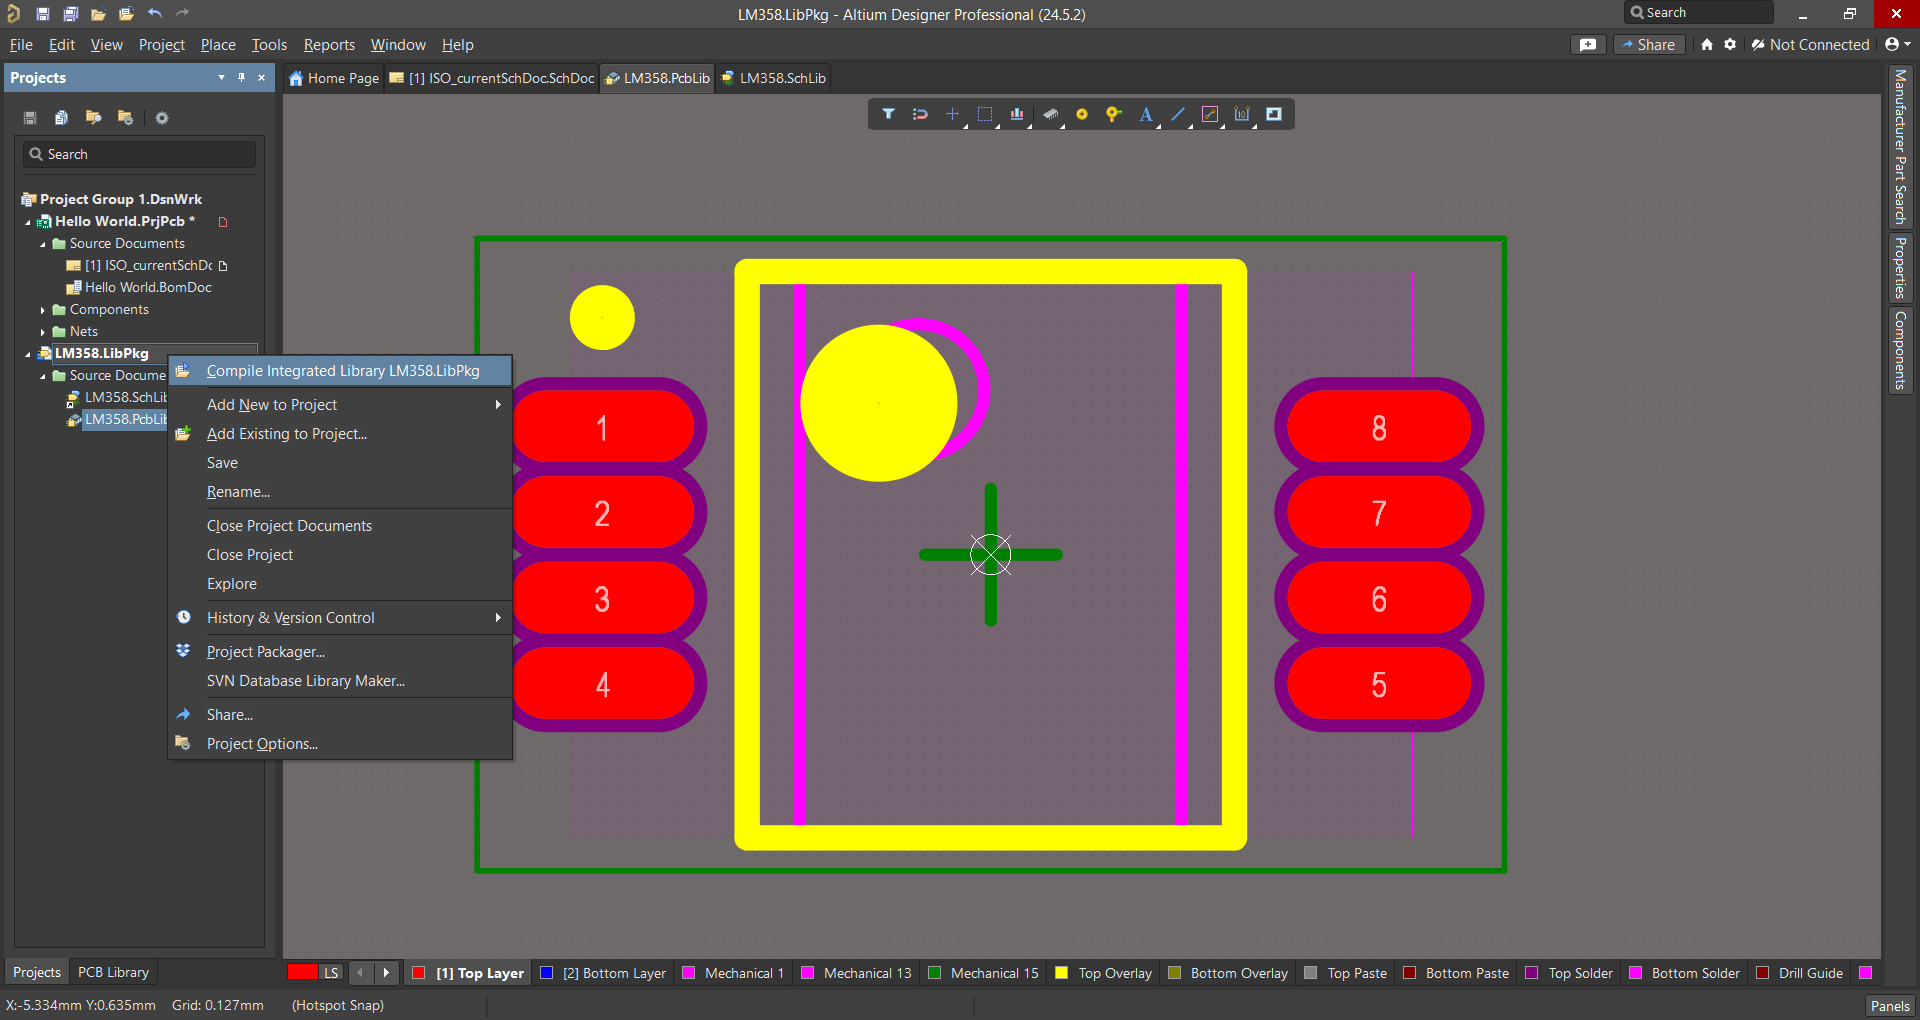
\includegraphics[width=1\textwidth]{pictures/ch3.16.png}
                \end{figure}
                \begin{figure}[H]
                    \centering
                    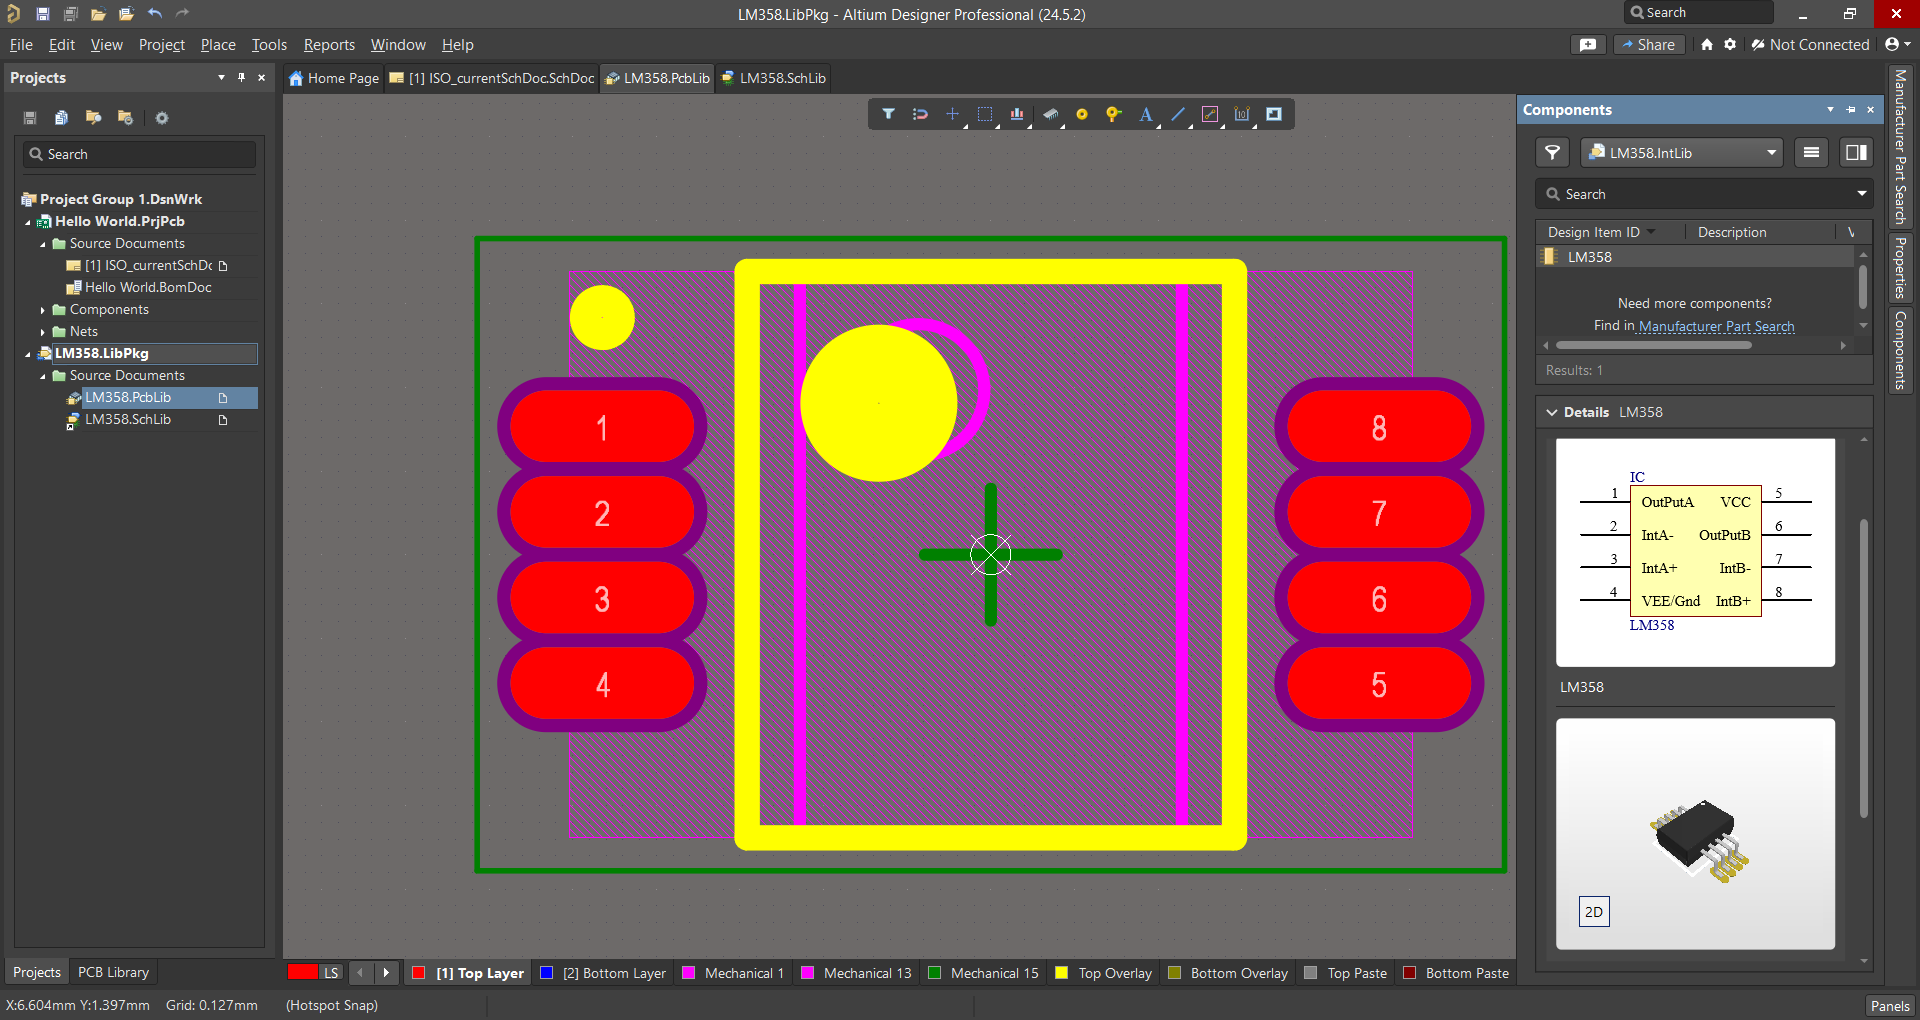
\includegraphics[width=1\textwidth]{pictures/ch3.14.png}
                    \caption{Hoàn tất việc tạo thư viện schematic và PCB 3D cho LM358} 
                \end{figure}
                \cleardoublepage
    \chapter{TẠO THƯ VIỆN SCHEMATIC VÀ PCB 3D}
    \section{Trình tự tạo thư viện schematic}
        Bước 1: Chọn File/New/Library để tạo thư viện mới.
        \begin{figure}[H]
            \centering
            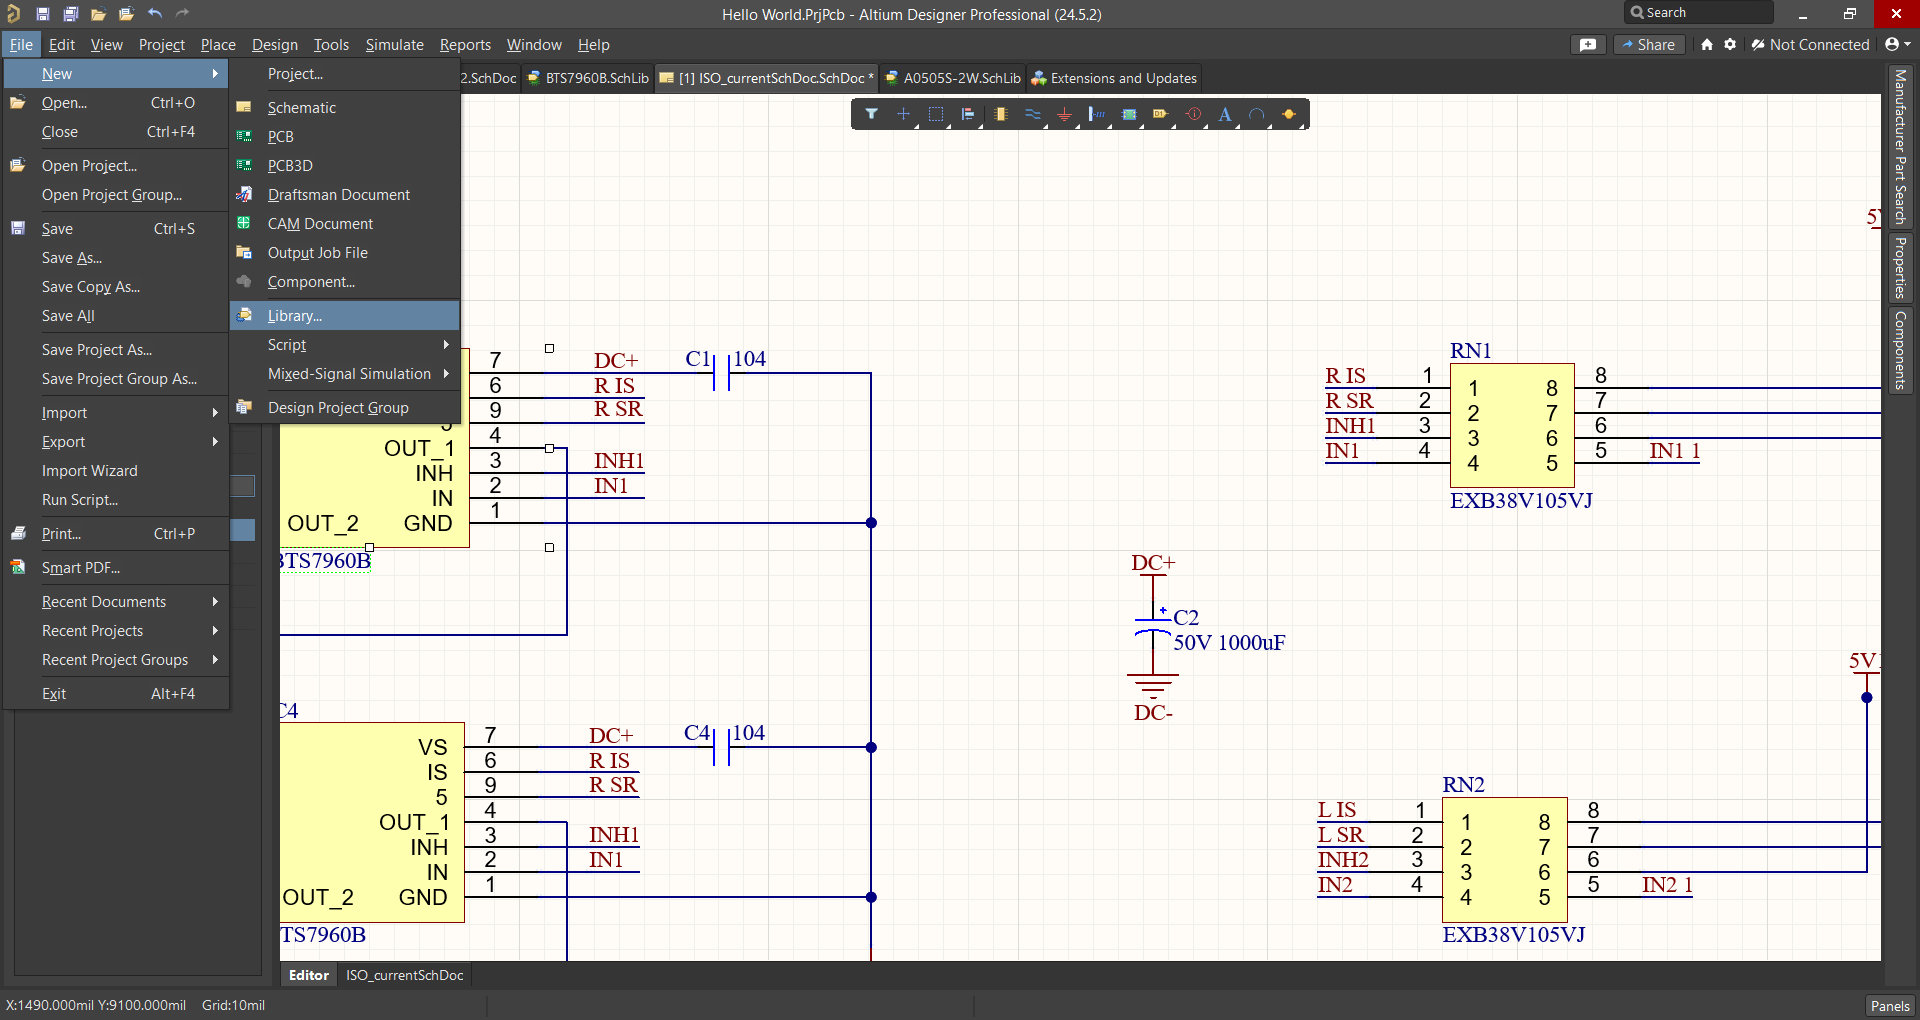
\includegraphics[width=1\textwidth]{pictures/ch3.1.png}
        \end{figure}
        Bước 2: Chọn Schematic Library và nhấn Create.
        \begin{figure}[H]
            \centering
            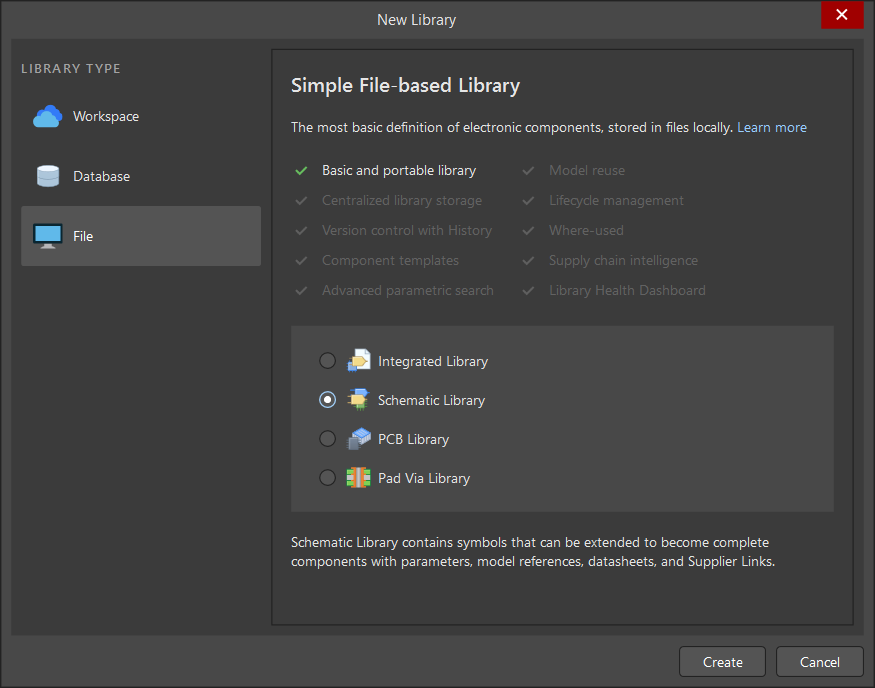
\includegraphics[width=0.8\textwidth]{pictures/ch3.2.png}
        \end{figure}
        Bước 3: Vẽ khối và đặt các chân theo hướng dẫn của datasheet.
        \begin{figure}[H]
            \centering
            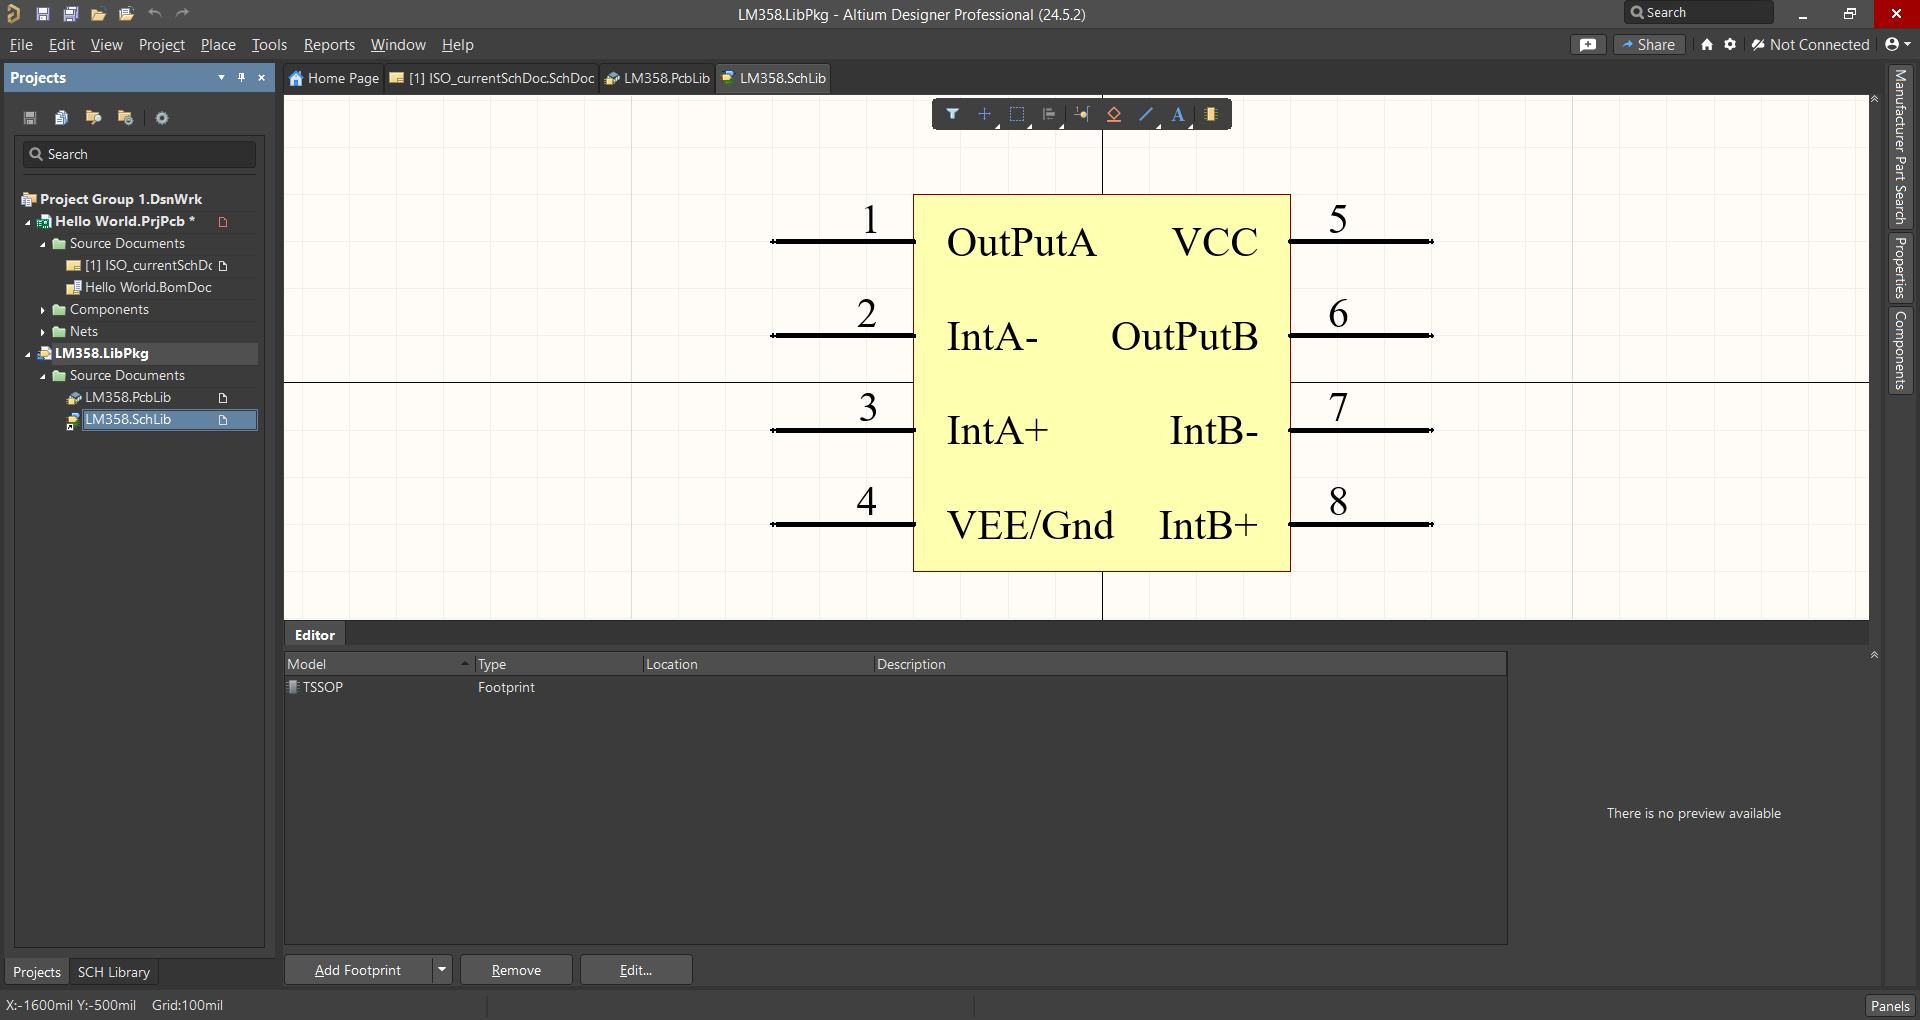
\includegraphics[width=1\textwidth]{pictures/ch3.3.png}
        \end{figure}
        Bước 4: Đặt tên cho thư viện và lưu lại.\\
    \section{Trình tự tạo thư viện PCB }
        \textbf{Ví dụ: Tạo thư viện fPCB 3D cho LM358 SOP8.}\\
        Bước 1: Chọn File/New/Library để tạo thư viện mới.\\
        Bước 2: Chọn PCB Library và nhấn Create.
        \begin{figure}[H]
            \centering
            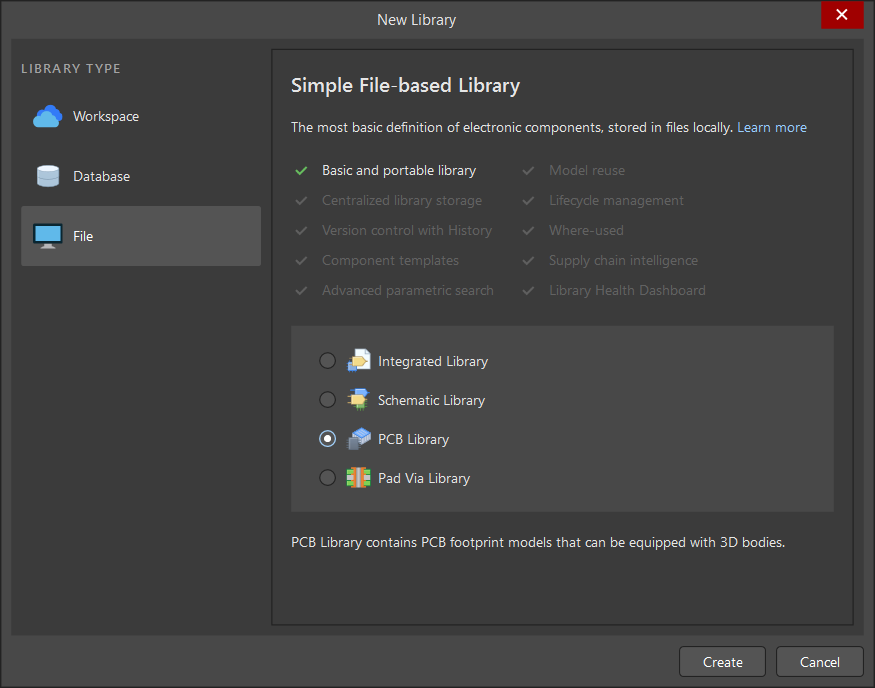
\includegraphics[width=0.7\textwidth]{pictures/ch3.4.png}
        \end{figure}
        Bước 3: Chọn Tools/IPC Compliant Footprint Wizard/Next.
        \begin{figure}[H]
            \centering
            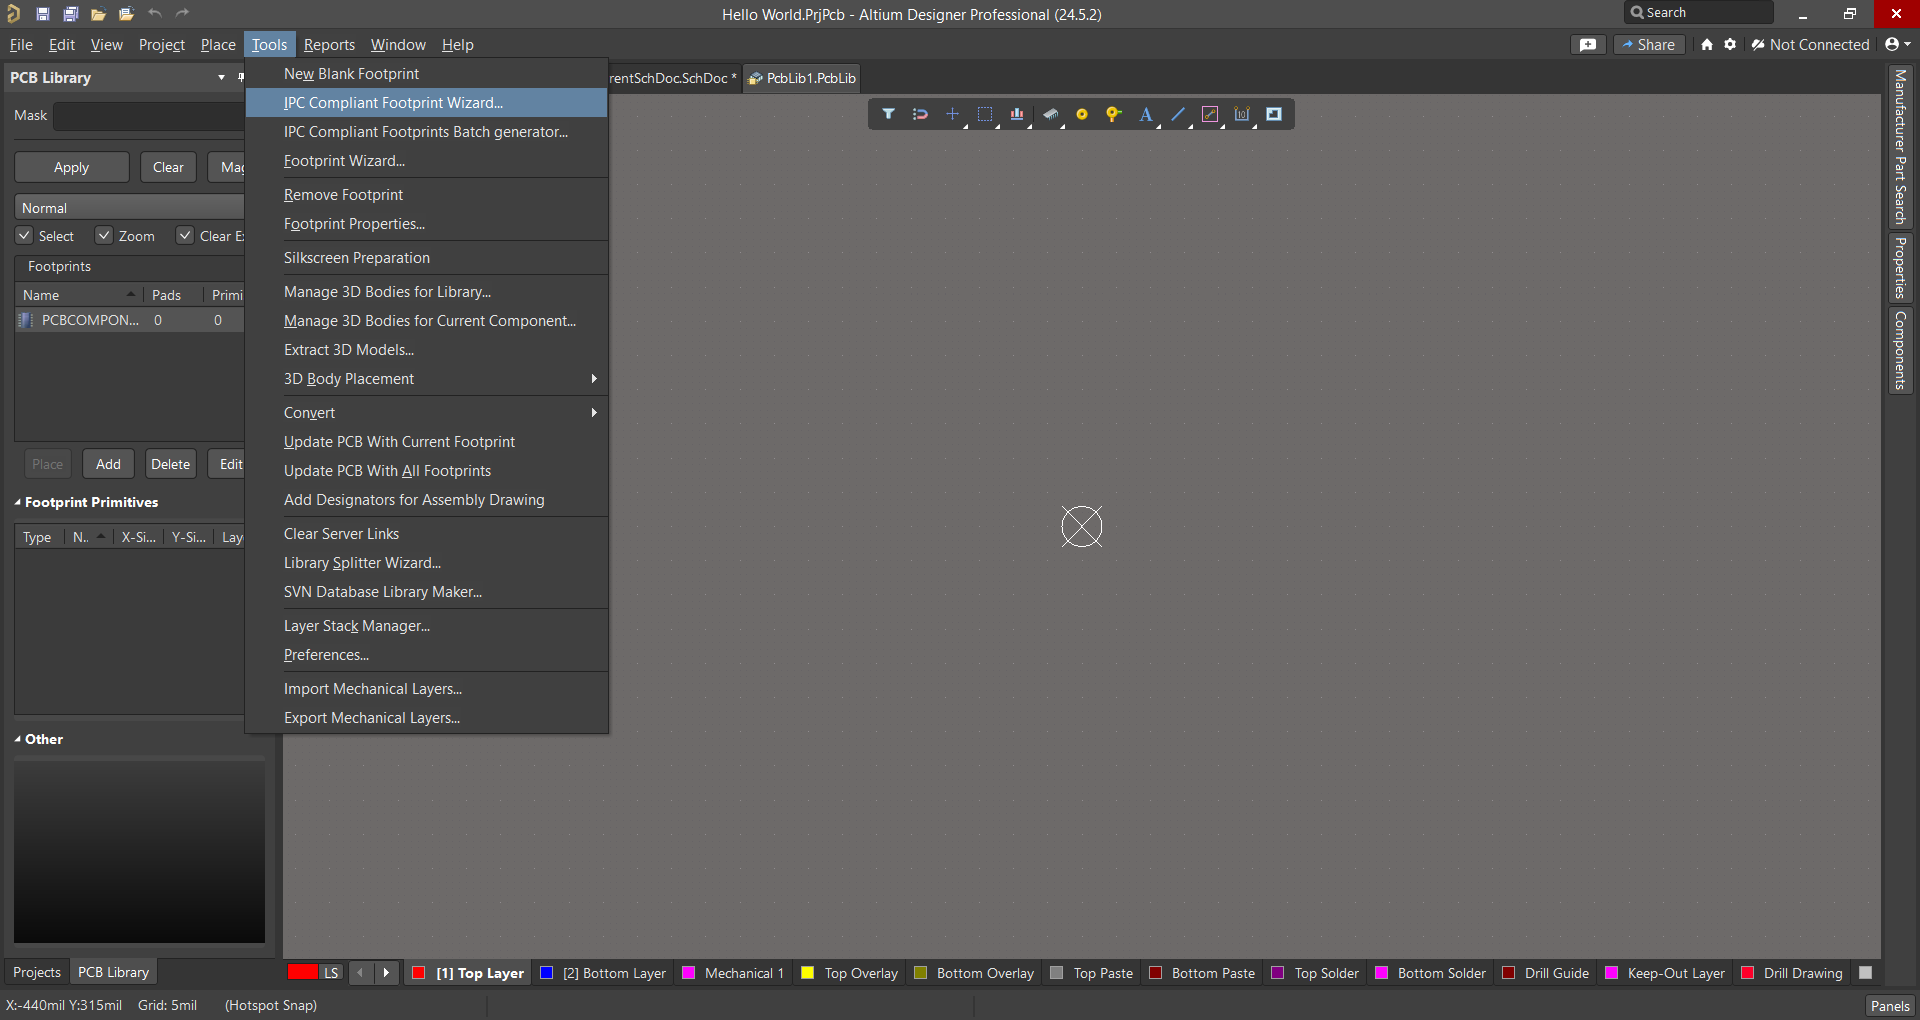
\includegraphics[width=1\textwidth]{pictures/ch3.5.png}
        \end{figure}
        Bước 4: Chọn kiểu chân SOP/TSOP và nhấn NEXT.
        \begin{figure}[H]
            \centering
            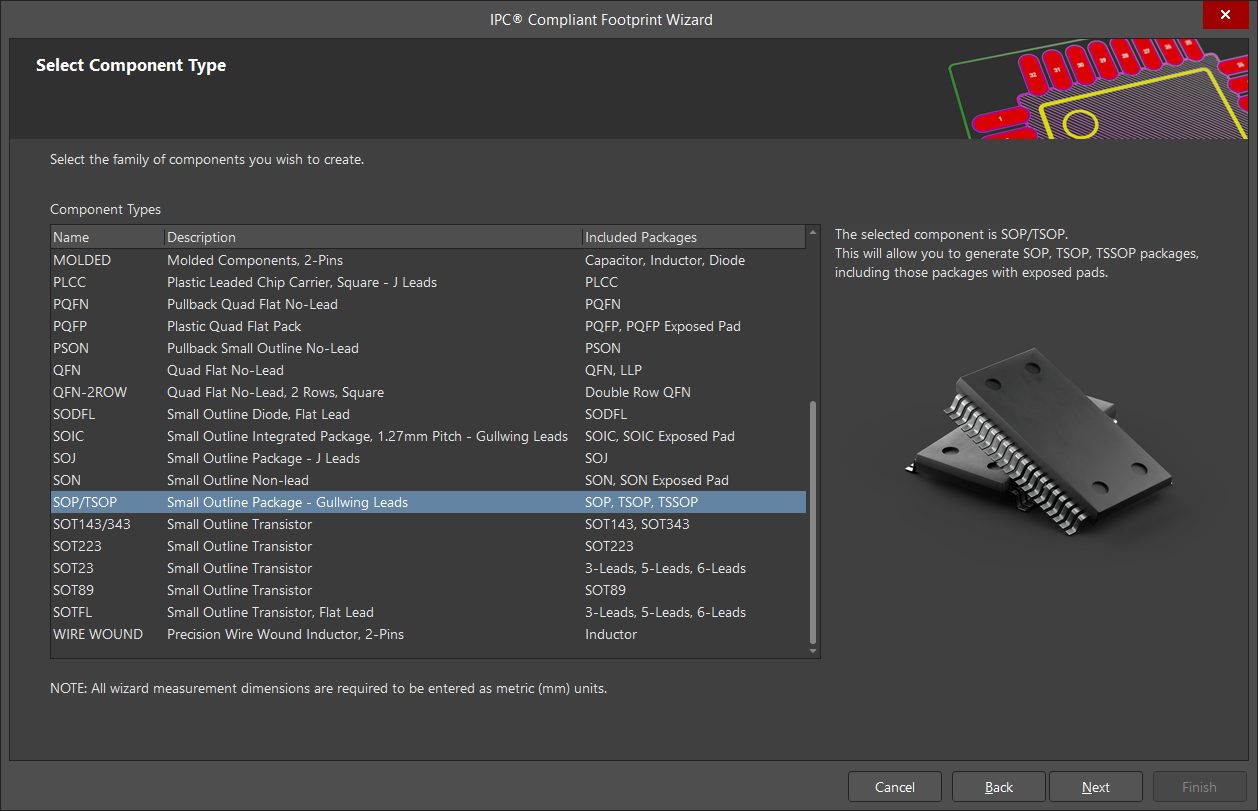
\includegraphics[width=1\textwidth]{pictures/ch3.6.png}
        \end{figure}
        \cleardoublepage
        Bước 5: Đọc datasheet của linh kiện để tìm các thông số thiết kế.
        \begin{figure}[H]
            \centering
            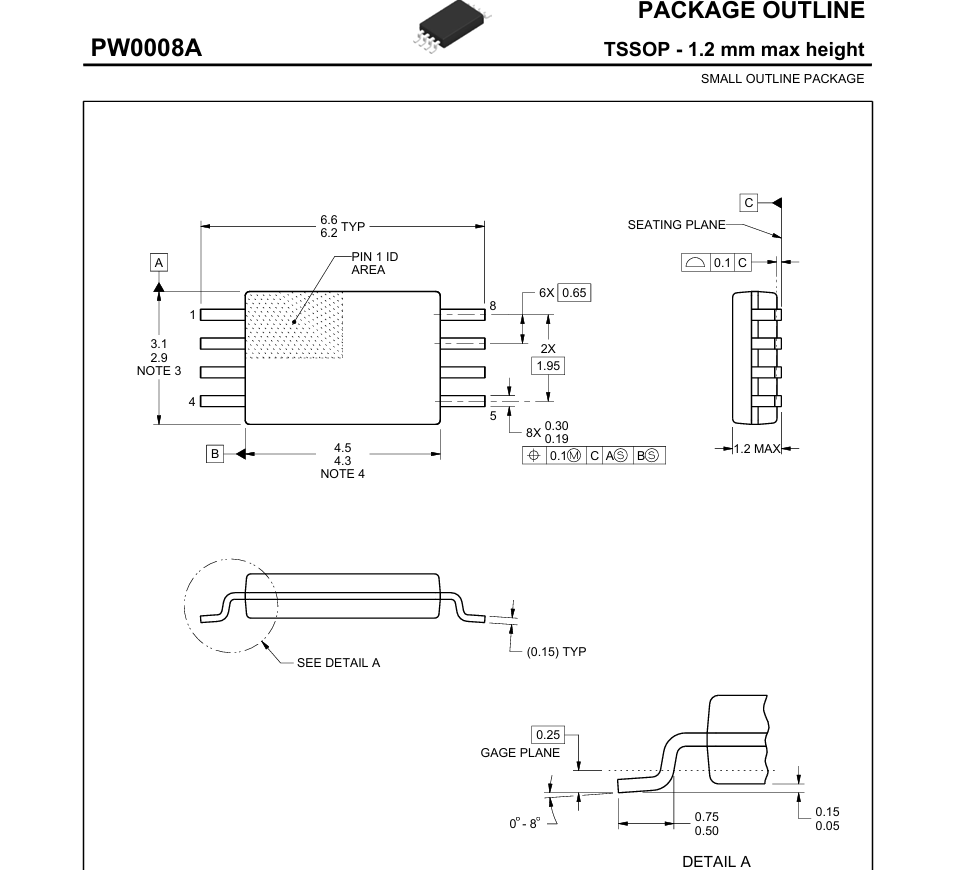
\includegraphics[width=0.9\textwidth]{pictures/ch3.7.png}
        \end{figure}
        Bước 6: Nhập các thông số vào các ô tương ứng và nhấn NEXT.
        \begin{figure}[H]
            \centering
            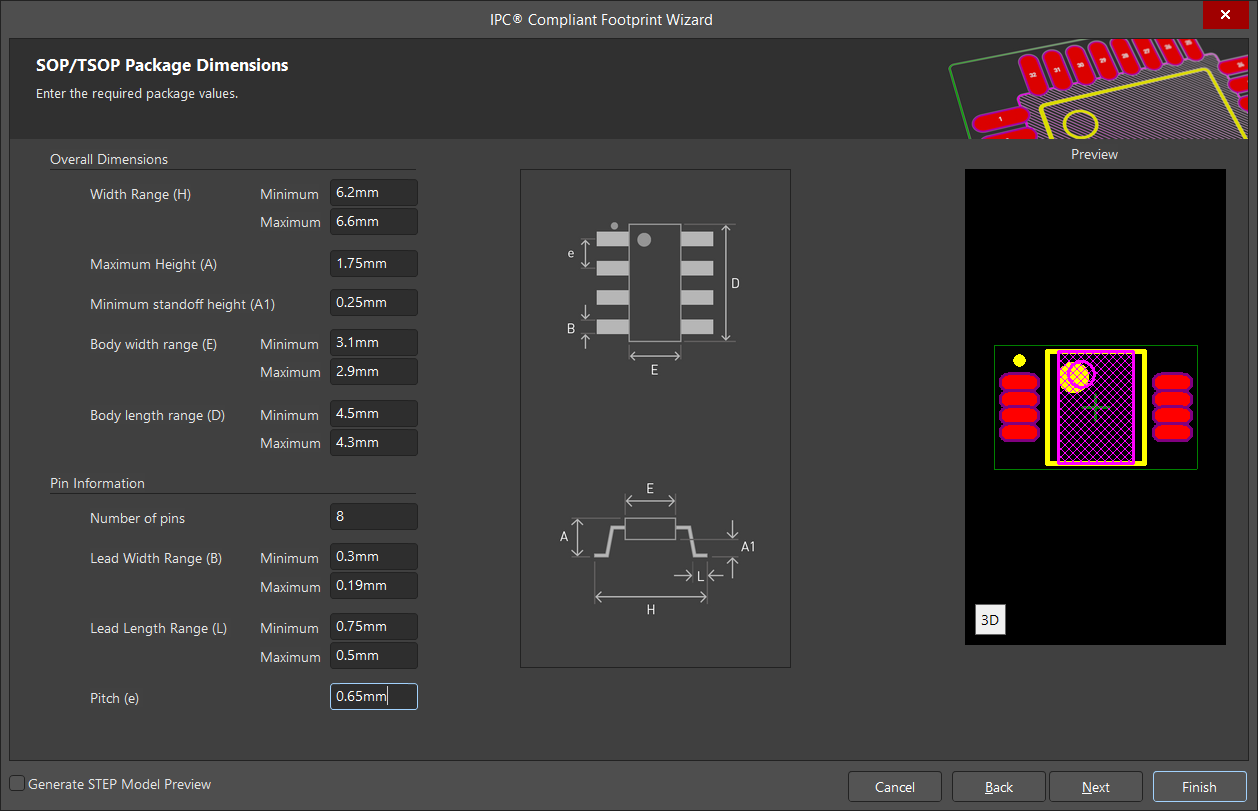
\includegraphics[width=0.8\textwidth]{pictures/ch3.8.png}
        \end{figure}
        Bước 7: Tiếp tục nhấn NEXT cho đến khi đến màn hình lưu và đặt tên.
        \begin{figure}[H]
            \centering
            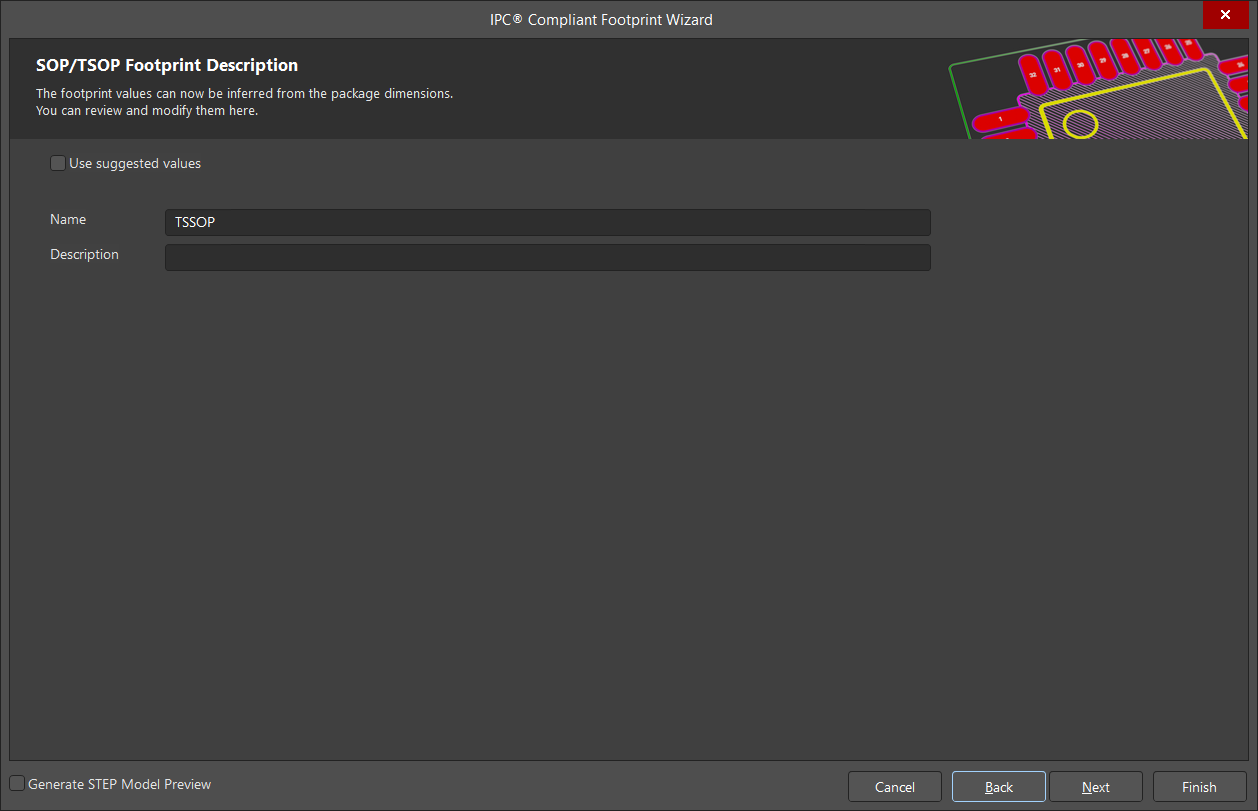
\includegraphics[width=1\textwidth]{pictures/ch3.9.png}
        \end{figure}
        Bước 8: Chọn Produce 3D/STEP model nhấn NEXT và FINISH.
        \begin{figure}[H]
            \centering
            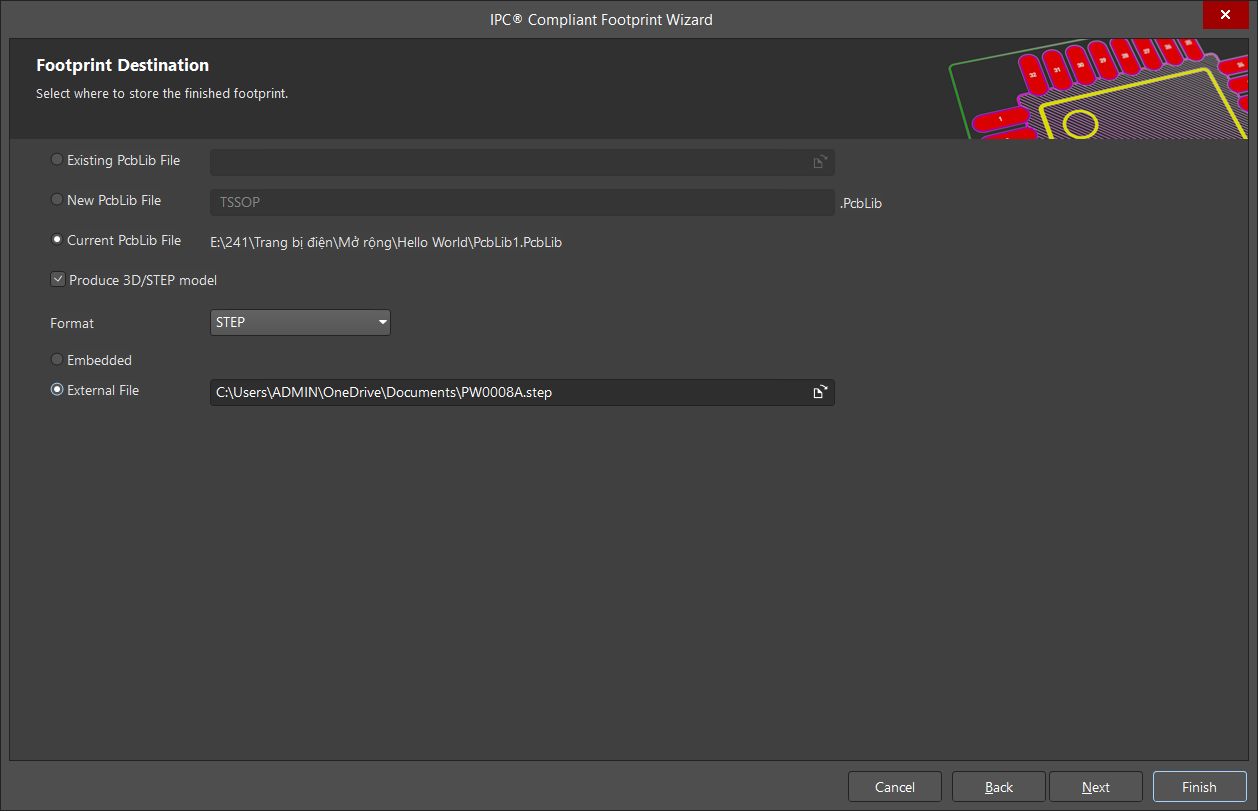
\includegraphics[width=1\textwidth]{pictures/ch3.10.png}
        \end{figure}
        \cleardoublepage
        Bước 9: Hoàn thành việc tạo thư viện footprint cho linh kiện LM358 SOP8.
        \begin{figure}[H]
            \centering
            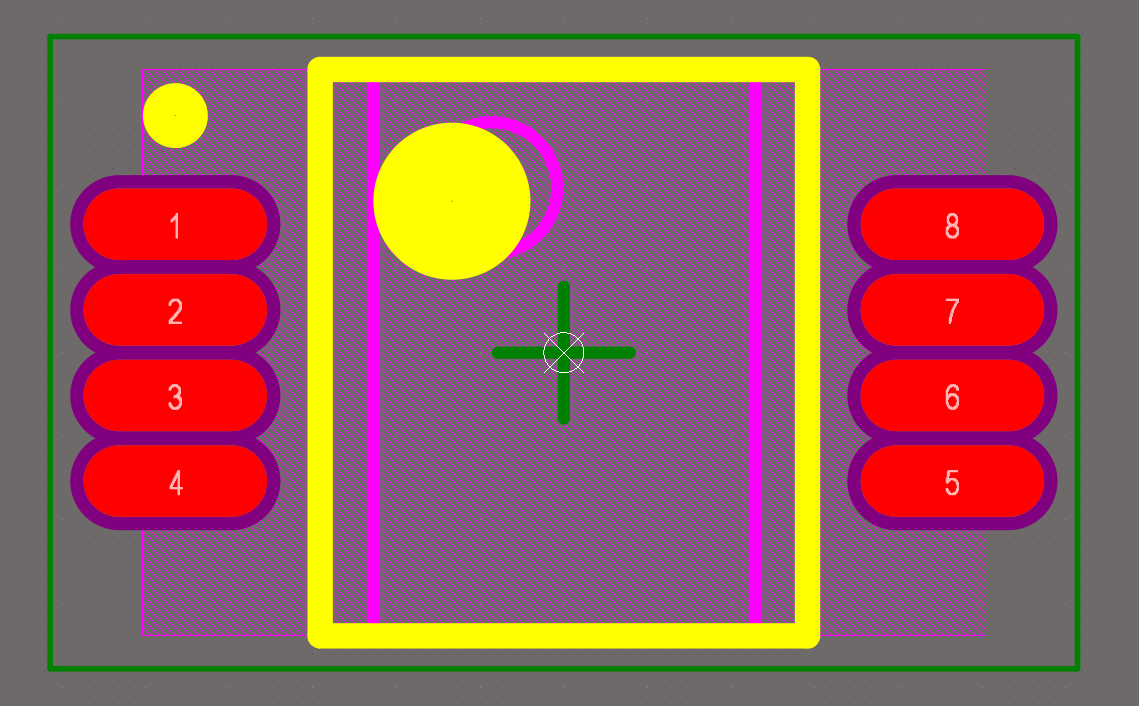
\includegraphics[width=0.9\textwidth]{pictures/ch3.11a.png}
            \caption{Footprint LM358 SOP8 vừa tạo} 
        \end{figure}
        \begin{figure}[H]
            \centering
            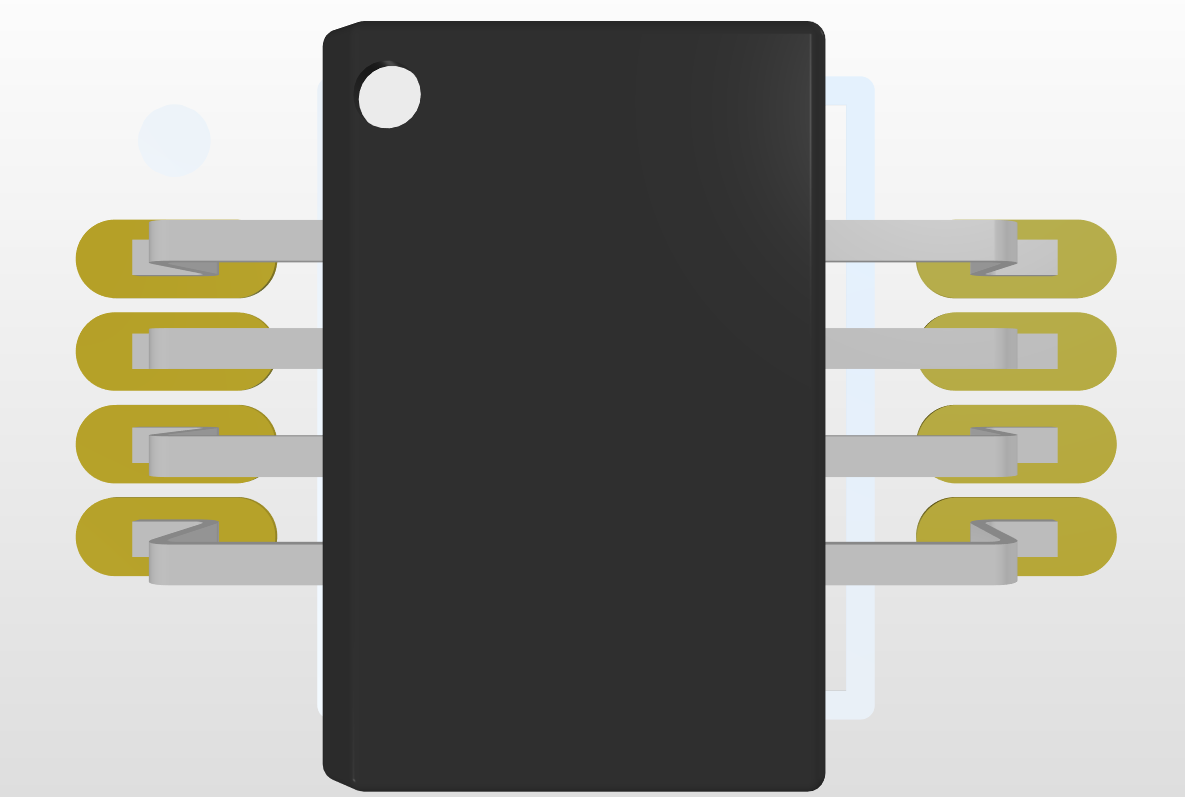
\includegraphics[width=0.9\textwidth]{pictures/ch3.11b.png}
            \caption{Mô hình PCB 3D LM358 SOP8 vừa tạo}
        \end{figure}
        \cleardoublepage
    \section{Add thư viện schematic và thư viện PCB lại với nhau}
        Bước 1: Ở màn hình làm việc của thư viện schematic chọn Add Footprint.
        \begin{figure}[H]
            \centering
            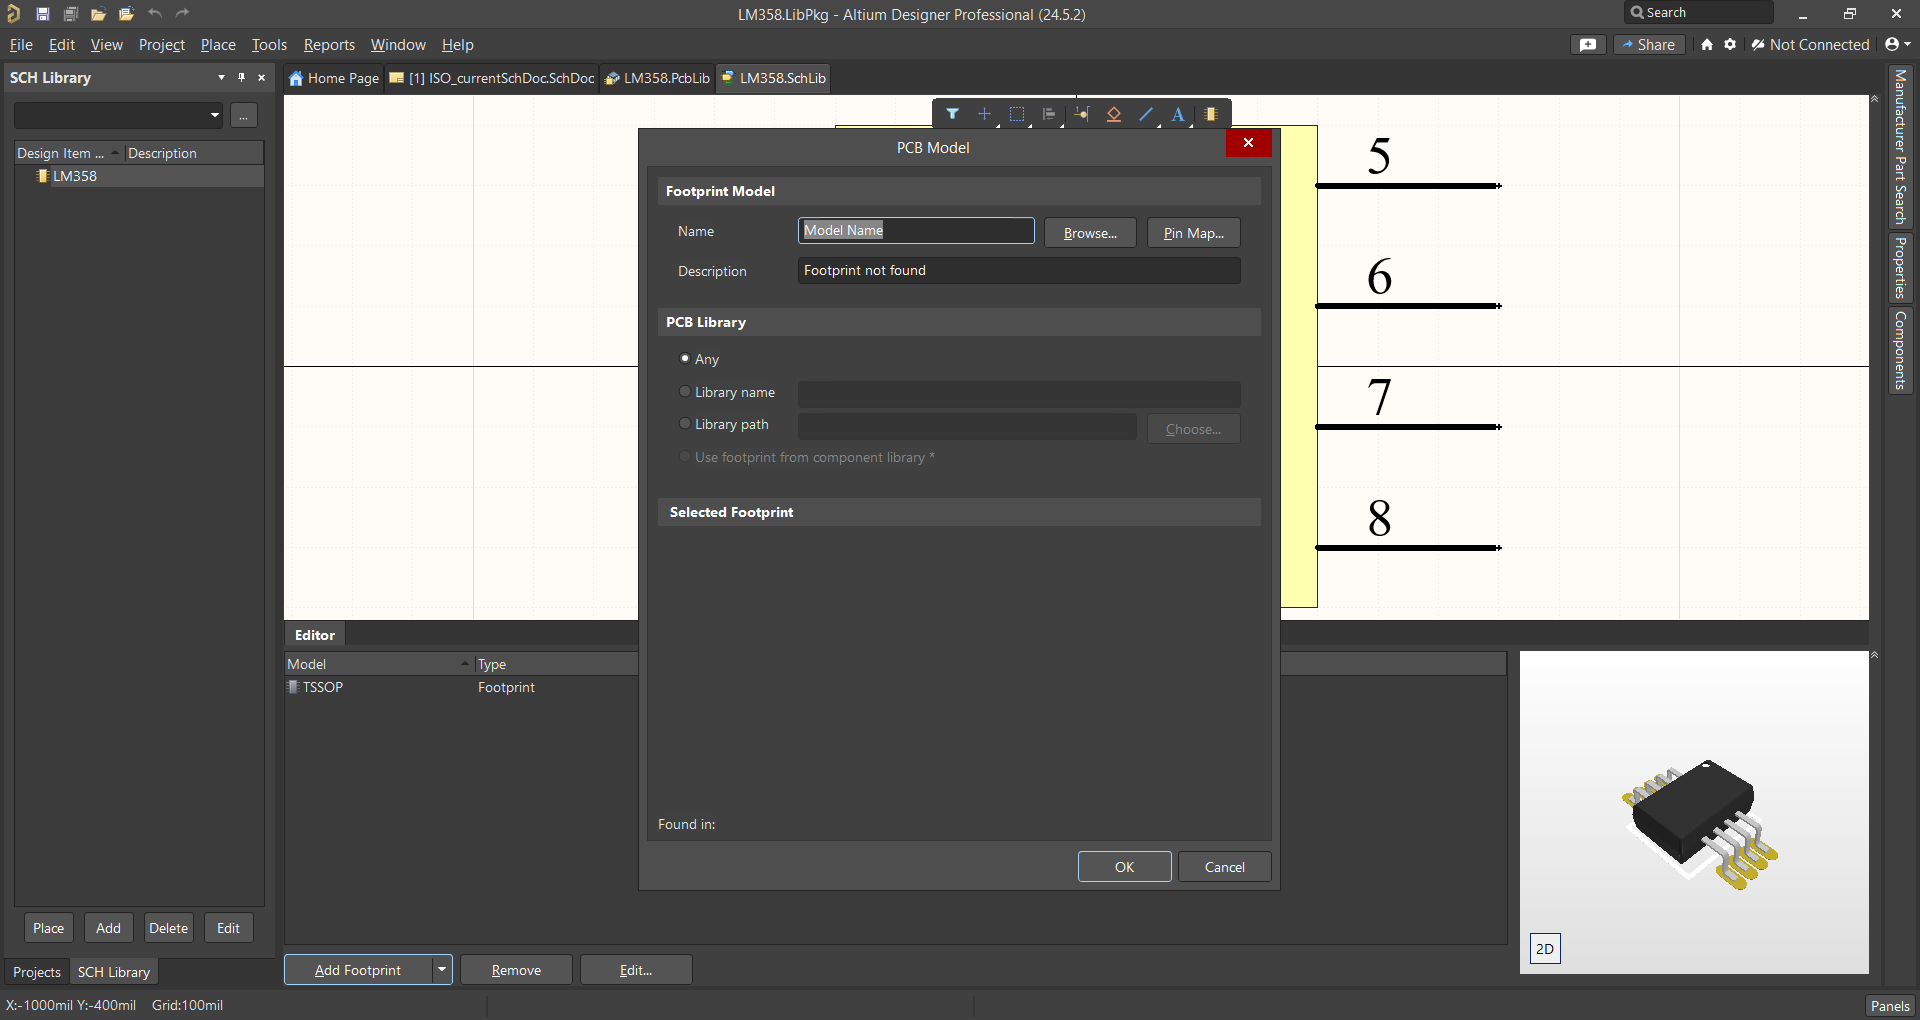
\includegraphics[width=1\textwidth]{pictures/ch3.12.png}
        \end{figure}
        Bước 2: Chọn Browse và chọn thư viện PCB tương ứng và nhấn OK
        \begin{figure}[H]
            \centering
            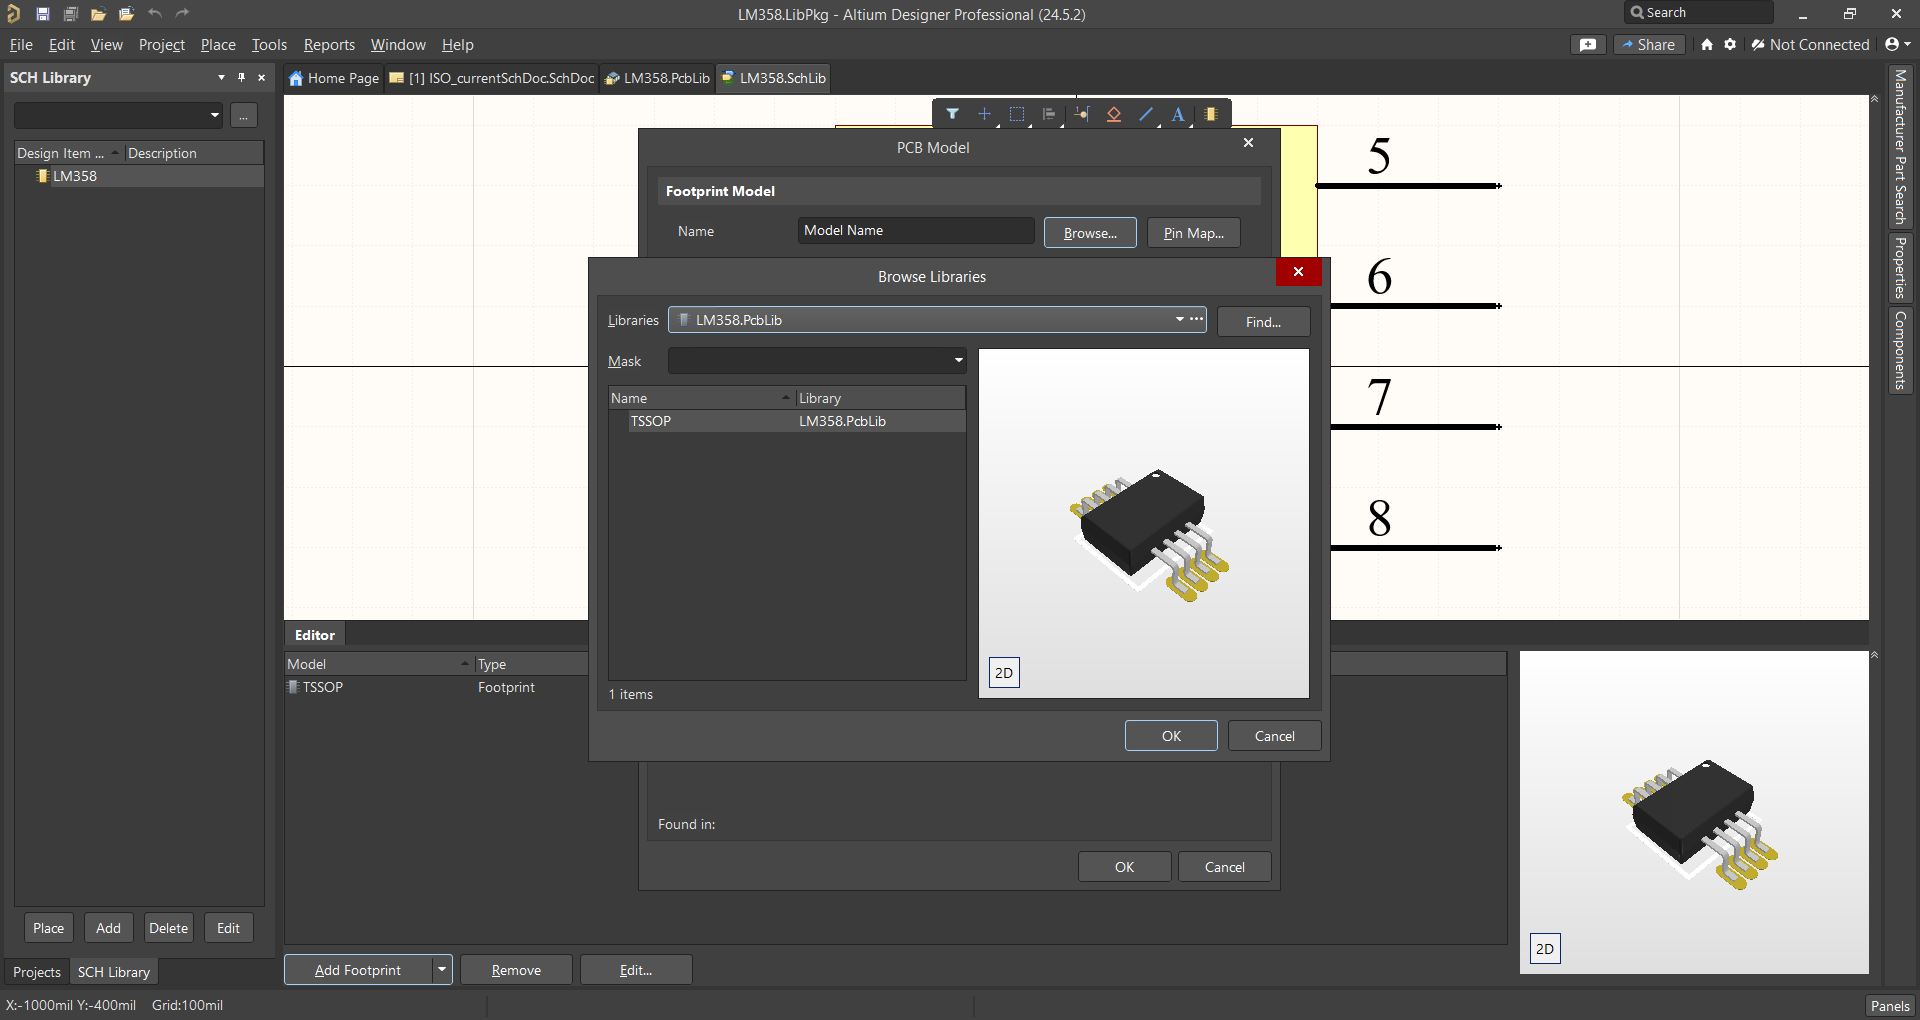
\includegraphics[width=1\textwidth]{pictures/ch3.13.png}
        \end{figure}
        \cleardoublepage
        Bước 3: Vào File/New chọn Library và chọn Integrated Library.
        \begin{figure}[H]
            \centering
            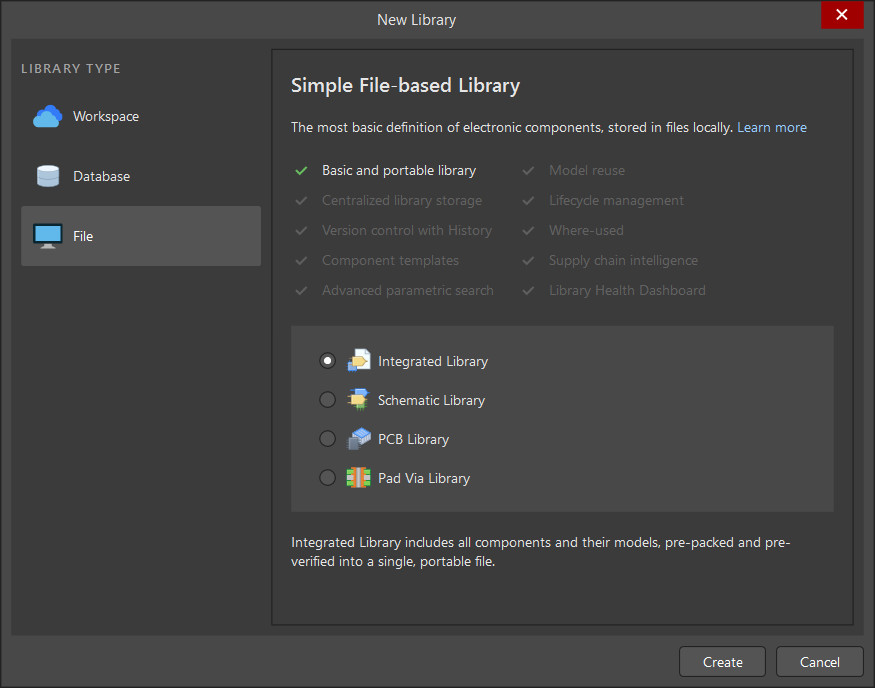
\includegraphics[width=1\textwidth]{pictures/ch3.15.png}
        \end{figure}
        Bước 4: Kéo 2 thư viện schematic và PCB vào Integrated Library vừa tạo và lưu lại. 
        Bước 5: Click chuột phải và chọn Compile Integrated Library.
        \begin{figure}[H]
            \centering
            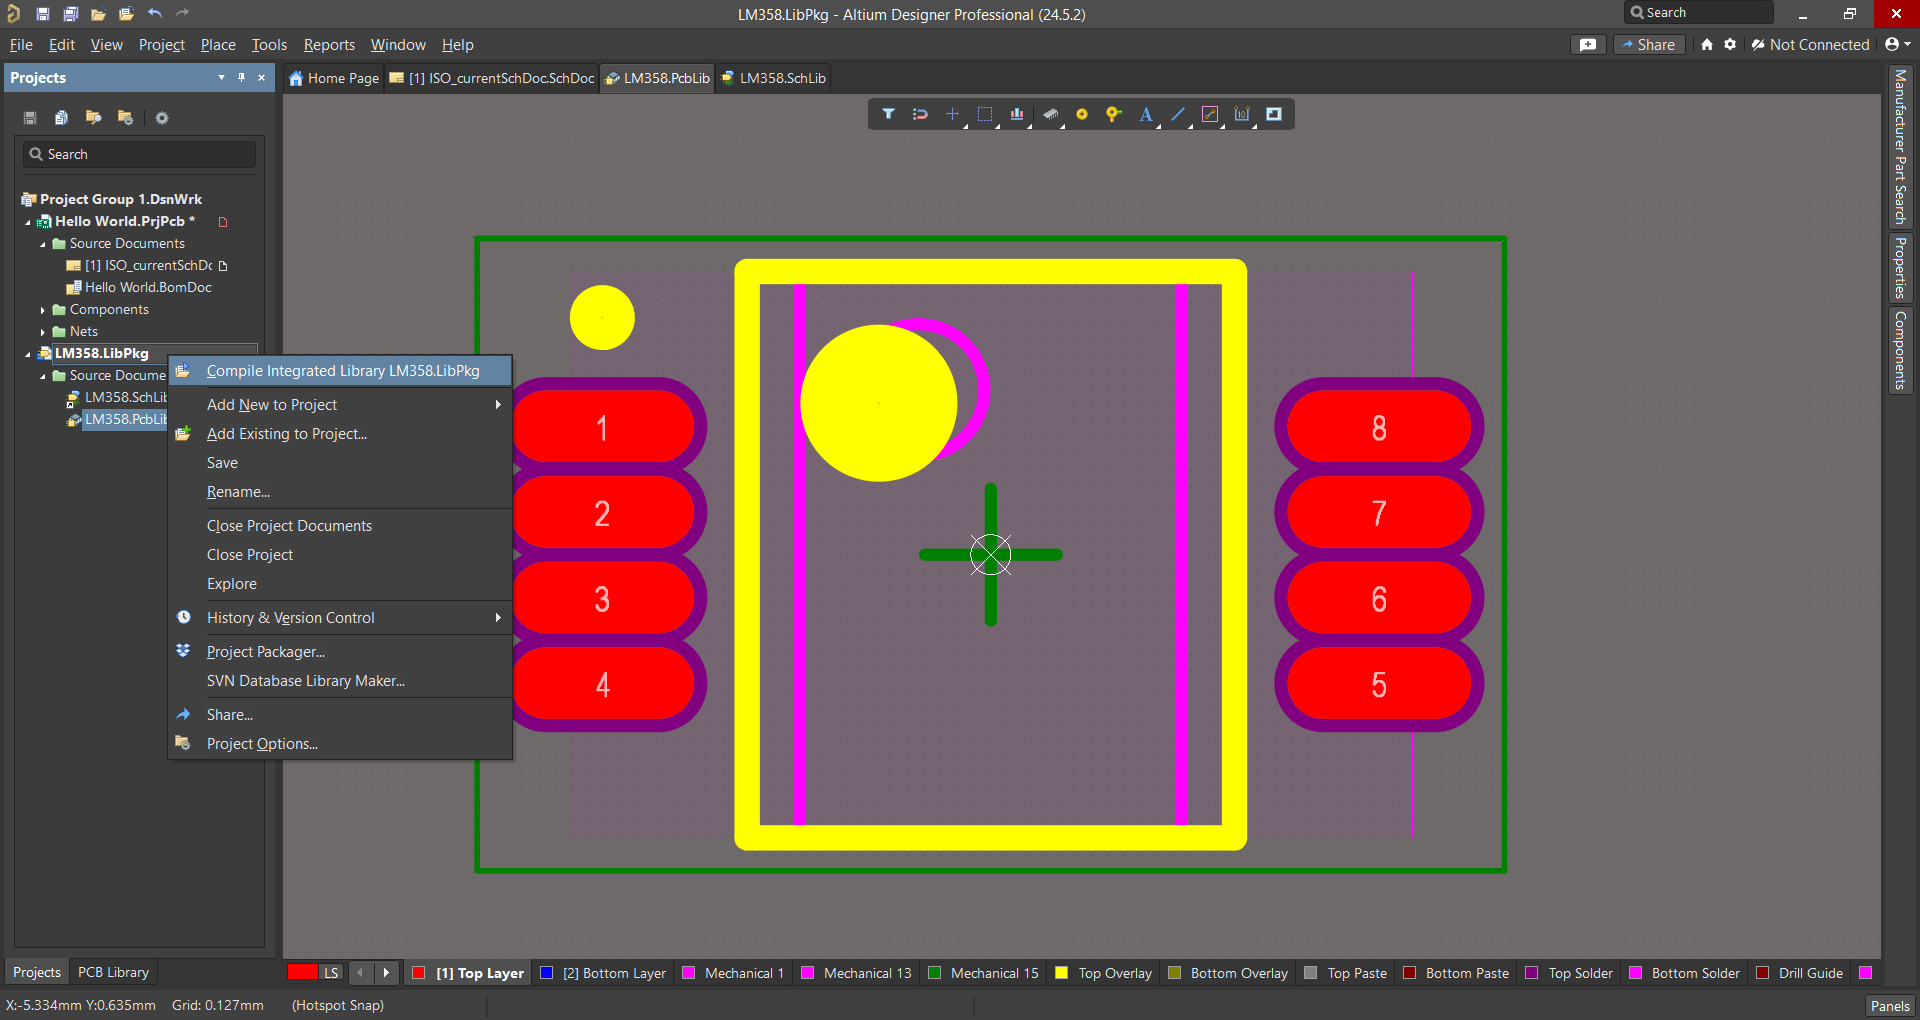
\includegraphics[width=1\textwidth]{pictures/ch3.16.png}
        \end{figure}
        \begin{figure}[H]
            \centering
            \includegraphics[width=1\textwidth]{pictures/ch3.14.png}
            \caption{Hoàn tất việc tạo thư viện schematic và PCB 3D cho LM358} 
        \end{figure}
        \cleardoublepage
    \chapter{MẠCH CẦU H}
    \section{Cấu tạo của mạch cầu H}
        Mạch cầu H là một mạch điện tử cơ bản được sử dụng rộng rãi để điều khiển hướng quay của động cơ một chiều (DC) hoặc điều khiển công suất truyền đến tải. Hình dạng mạch khi vẽ ra giống chữ H, nên được gọi là mạch cầu H.\\
        Mạch cầu H, như tên gọi của nó, được thiết kế với cấu trúc cơ bản hình chữ H. Cấu tạo chính của mạch bao gồm: 
        \vspace{-0.4cm}
        \begin{itemize}
            \item 4 công tắc điện tử: Đây là các linh kiện chính của mạch, thường là transistor (BJT) hoặc MOSFET. Chúng đóng vai trò như những chiếc cầu nối, điều khiển dòng điện đi qua động cơ.
            \item Diode bảo vệ: Các diode được mắc song song với mỗi công tắc để bảo vệ chúng khỏi hiện tượng điện áp ngược khi các công tắc tắt.
            \item Nguồn cung cấp: Cung cấp điện áp một chiều để cấp cho mạch và động cơ.
        \end{itemize}
        \begin{figure}[H]
            \centering
            \includegraphics[width=0.4\textwidth]{pictures/cauhsimple.png}
            \caption{Mạch cầu H đơn giản}
            \label{fig:hbridge}
        \end{figure}
        \begin{figure}[H]
            \centering
            \includegraphics[width=0.5\textwidth]{pictures/cauhcurcuit.png}
            \caption{Các mô đun có tích hợp mạch cầu H}
            \label{fig:hbridge}
        \end{figure}
        \cleardoublepage
        \subsection{Nguyên lý hoạt động của mạch cầu H}
        \begin{figure}[H]
            \centering
            \includegraphics[width=0.8\textwidth]{pictures/cauhwork.png}
            \caption{Nguyên lý hoạt động của mạch cầu H}
            \label{fig:hbridge}
        \end{figure}
        \hspace*{0.6cm}Trong mô hình này, chúng ta sử dụng mạch cầu H để điều khiển động cơ một chiều. Động cơ DC có thể quay theo chiều thuận hoặc chiều nghịch, tùy thuộc vào cách chúng ta kết nổi cực âm và cực dương cho động cơ.

        Mạch cầu H được thiết kế để điều khiển động cơ DC hoặc tải điện theo hai hướng: hướng thuận và hướng nghịch. Mạch này bao gồm bốn transistor hoặc MOSFET được kết nối với nhau theo cấu trúc dạng cầu.

        Khi một cặp transistor được kích hoạt, một transistor ở phía trên và một transistor ở phía dưới, dòng điện sẽ chảy qua động cơ theo hướng tương ứng. Khi cặp transistor khác được kích hoạt, hướng dòng điện sẽ đảo ngược, từ đó điều khiển tải đi theo hướng khác

        Việc điều khiển được thực hiện thông qua các cổng điều khiển được kết nối đến bồn transistor hoặc MOSFET, khi điện áp được đưa vào các cổng này, các transistor sẽ được kích hoạt hoặc ngưng hoạt động tùy thuộc vào tín hiệu đầu vào tại cổng.
        \cleardoublepage
    \section{Ứng dụng mạch cầu H trong thực tế}
        Bên cạnh việc điều khiển động cơ DC, mạch cầu H còn được sử dụng rộng rãi trong các ứng dụng khác như:
        \begin{itemize}
            \item Điều khiển động cơ servo: Mạch cầu H cũng được sử dụng để điều khiển động cơ servo trong các ứng dụng yêu cầu độ chính xác cao như robotica, máy bay điều khiển từ xa và các thiết bị tự động hóa khác.
            \item Hệ thống quản lý năng lượng: Mạch cầu H được tích hợp vào hệ thống quản lý năng lượng để điều khiển việc cung cấp năng lượng cho các thiết bị điện tử như ổ đĩa động cơ, hệ thống điều hòa không khí và thiết bị gia dụng.
            \item Hệ thống truyền dẫn điện không dây: Trong các ứng dụng truyền dẫn điện không dây như sạc không dây cho điện thoại di động, mạch cầu H có thể được sử dụng để điều khiển nguồn điện được truyền từ trạm sạc đến thiết bị di động.
            \item Hệ thống giao thông thông minh: Trong các hệ thống giao thông thông minh, mạch cầu H có thể được sử dụng để điều khiển các thiết bị như cổng xoay, cửa tự động và đèn tín hiệu giao thông để tạo ra một mạng lưới giao thông hiệu quả và an toàn.
        \end{itemize}
        \begin{figure}[H]
            \centering
            \includegraphics[width=1\textwidth]{pictures/cong3que.png}
            \caption{Hệ thống cổng xoay 3 càng có sử dụng mạch cầu H}
            \label{fig:hbridge}
        \end{figure}
        \cleardoublepage
    \chapter{ENCODER VÀ ỨNG DỤNG TRONG ĐIỀU KHIỂN ĐỘNG CƠ}
    \section{Khái niệm encoder}
        Encoder là một bộ cảm biến chuyển động cơ học tạo ra tín hiệu analog hoặc tín hiệu kỹ thuật số (digital) đáp ứng với chuyển động. Encoder có khả năng biến đổi chuyển động (chuyển động tịnh tiến, chuyển động quay của trục, ...) thành tín hiệu đầu ra số hoặc xung. Các thông tin được encoder chuyển đổi trong động cơ bao gồm
        \begin{itemize}
            \item Tốc độ quay của động cơ.
            \item Vị trí: độ dịch chuyển của trục động cơ so với vị trí ban đầu.
            \item Hướng quay: Tùy thuộc vào từng loại encoder.
        \end{itemize}


        \section{Phân loại}
        Các bộ mã hóa encoder có thể được phân thành các loại
        \begin{itemize}
            \item Bộ mã hóa quay (Rotary Encoder): hay còn gọi là bộ mã hóa trục, thu thập dữ liệu và cung cấp phản hồi dựa trên chuyển động quay của 1 đối tượng. Các lĩnh vực có nhu cầu sử dụng rotary encoder phải kể đến phản hồi động cơ, cánh tay robot. Rotary encoder được phân loại thành 2 loại là bộ mã hóa gia tăng (incremetal encoder) và tuyệt đối (absolute encoder). Bộ mã hóa gia tăng cung cấp thông tin vị trí góc tương đối bằng cách tạo ra một loạt xung khi trục quay, trong khi bộ mã hóa tuyệt đối cung cấp giá trị vị trí duy nhất cho mỗi vị trí trục, đảm bảo các phép đo chính xác và có thể lặp lại. 
            \begin{figure}[H]
                \centering
                \includegraphics[width=1\textwidth]{pictures/encoder1.png}
            \end{figure}
            \begin{figure}[H]
                \centering
                \includegraphics[width=1\textwidth]{pictures/encoder2.png}
            \end{figure}
            \item Bộ mã hóa tuyến tính (Linear encoders) được thiết kế để đo vị trí dọc theo đường thẳng, chúng thường được sử dụng trong máy CNC, dụng cụ đo chính xác và dây chuyền lắp ráp tự động. Encoder tuyến tính có thể là quang học hoặc từ tính. Bộ mã hóa quang học cung cấp độ phân giải và độ chính xác cao.
            \begin{figure}[H]
                \centering
                \includegraphics[width=0.7\linewidth]{pictures/encoder3.png}
            \end{figure}
        \end{itemize}
        Ngoài những phân loại chính, thì còn có phân loại theo những công nghệ dùng cho encoder, phổ biến là
        \begin{itemize}
            \item Quang học (Optical): Được sử dụng rộng rãi và phổ biến.
            \item Từ tính (Magnetic)
            \item Cơ học (Mechanical)
        \end{itemize}   
    \section{Cấu tạo của encoder}
        Mỗi loại bộ mã hóa (encoder) sẽ có thành phần chính và chức năng khác nhau, nhưng nhìn chung có 3 thành phần chính sau:
        \begin{itemize}
            \item Nguồn phát sáng (lightsource): là 1 đèn LED.
            \item Đĩa mã hóa (code disk): có rãnh nhỏ quay quanh trục, khi đĩa này quay và chiếu đèn LED lên trên mặt đĩa thì sẽ có sự ngắt quãng xảy ra. Các rãnh trên đĩa chia vòng tròn $360^{\circ}$ thành các góc bằng nhau. Một đĩa có thể có nhiều dãy rãnh tính từ tâm tròn.
            \item Bộ cảm biến ánh sáng thu tín hiệu (photosensor): là một con mắt thu quang điện để nhận tín hiệu từ đĩa quay
            \item  Bo mạch điện tử (electronic board): giúp khuếch đại tín hiệu
        \end{itemize}
        \begin{figure}[H]
                \centering
                \includegraphics[width=1\linewidth]{pictures/encoder5.png}
            \end{figure}
        
        
        \cleardoublepage
        \section{Nguyên lý hoạt động của encoder}
        Encoder quay sử dụng quang học hoạt động theo nguyên lý đĩa quay quanh trục. Trên đĩa mã hóa có các rãnh nhỏ để nguồn phát sáng chiếu tín hiệu quang qua đĩa. Chỗ có rãnh thì ánh sáng xuyên qua được, chỗ không có rãnh ánh sáng không xuyên qua được.
        Với các tín hiệu có, hoặc không có ánh sáng chiếu qua, người ta ghi nhận được đèn led có chiếu qua lỗ hay không. Số xung đếm được và tăng lên được tính bằng số lần ánh sáng bị cắt.
        Cảm biến thu ánh sáng sẽ bật tắt liên tục để tạo ra các xung vuông. Việc sử dụng các bộ mã hóa sẽ ghi nhận lại số xung và tốc độ xung. Tín hiệu dạng xung sẽ được truyền về bộ xử lý trung tâm (vi xử lý, PLC,…) và từ đó kỹ sư cơ khí sẽ biết được vị trí và tốc độ của động cơ.
        \begin{figure}[H]
            \centering
            \includegraphics[width=0.8\linewidth]{pictures/encoder6.png}
        \end{figure}
        
        \cleardoublepage
    \chapter{TÌM HIỂU CÁC LINH KIỆN KHÁC}
    \section{Bộ điều chỉnh LM2576}
        \subsection{Giới thiệu}
            \hspace*{0.6cm}LM2576 là một bộ điều chỉnh điện áp chuyển mạch (switching regulator) hiệu suất cao, có thể cung cấp dòng điện lên đến 3A. Nó được thiết kế để giảm thiểu số lượng linh kiện ngoại vi và đơn giản hóa thiết kế mạch.
        \subsection{Đặc điểm kỹ thuật}
            \begin{itemize}
                \item Điện áp đầu vào: 4V đến 40V
                \item Điện áp đầu ra: 1.23V đến 37V
                \item Dòng điện đầu ra: lên đến 3A
                \item Hiệu suất chuyển đổi: lên đến 90%
                \item Tần số chuyển mạch: 52kHz
            \end{itemize}   
        \subsection{Sơ đồ chân}
            \begin{figure}[H]
                \centering
                \includegraphics[width=0.5\textwidth]{pictures/lm2576_pinout.png}
                \caption{Sơ đồ chân của LM2576}
            \end{figure}
        \subsection{Chức năng từng chân của LM2576}
            LM2576 có 5 chân với các chức năng như sau:
            
            \begin{itemize}
                \item \textbf{Chân 1 (VIN)}: Chân này là đầu vào điện áp. Điện áp đầu vào có thể dao động từ 4V đến 40V.
                \item \textbf{Chân 2 (Output)}: Chân này là đầu ra điện áp đã được điều chỉnh. Điện áp đầu ra có thể được điều chỉnh từ 1.23V đến 37V tùy thuộc vào cấu hình mạch.
                \item \textbf{Chân 3 (Ground)}: Chân này là chân nối đất (GND) của mạch.
                \item \textbf{Chân 4 (Feedback)}: Chân này được sử dụng để điều chỉnh điện áp đầu ra. Nó nhận tín hiệu phản hồi từ mạch để duy trì điện áp đầu ra ổn định.
                \item \textbf{Chân 5 (ON/OFF)}: Chân này được sử dụng để bật hoặc tắt bộ điều chỉnh. Khi chân này được kéo lên mức cao, bộ điều chỉnh sẽ tắt và khi kéo xuống mức thấp, bộ điều chỉnh sẽ bật.
            \end{itemize}

            
        \subsection{Ứng dụng}
            LM2576 được sử dụng rộng rãi trong các ứng dụng như:
            \begin{itemize}
                \item Bộ nguồn chuyển mạch
                \item Bộ điều chỉnh điện áp cho các thiết bị điện tử
                \item Hệ thống cung cấp điện cho vi điều khiển và các mạch số
            \end{itemize}
            
        \subsection{Sơ đồ mạch ứng dụng}
            \begin{figure}[H]
                \centering
                \includegraphics[width=0.8\textwidth]{pictures/lm2576_application_circuit.png}
                \caption{Sơ đồ mạch ứng dụng của LM2576}
            \end{figure}

        \subsection{Giải thích chức năng của mạch ứng dụng}
            \hspace*{0.6cm}Sơ đồ mạch ứng dụng của LM2576 bao gồm các thành phần chính như sau:
            
            \begin{itemize}
                \item \textbf{LM2576}: Bộ điều chỉnh điện áp chuyển mạch, là thành phần chính của mạch.
                \item \textbf{Cuộn cảm (L)}: Lưu trữ năng lượng khi transistor bên trong LM2576 bật và giải phóng năng lượng khi transistor tắt, giúp duy trì điện áp đầu ra ổn định.
                \item \textbf{Tụ điện đầu vào (C\textsubscript{in})}: Giúp lọc nhiễu và ổn định điện áp đầu vào.
                \item \textbf{Tụ điện đầu ra (C\textsubscript{out})}: Giúp lọc nhiễu và ổn định điện áp đầu ra.
                \item \textbf{Điện trở phản hồi (R\textsubscript{fb})}: Được sử dụng để điều chỉnh điện áp đầu ra bằng cách cung cấp tín hiệu phản hồi cho chân Feedback của LM2576.
                \item \textbf{Diode Schottky (D)}: Giúp chuyển đổi năng lượng từ cuộn cảm sang tải khi transistor bên trong LM2576 tắt.
            \end{itemize}
            
            \textbf{Nguyên lý hoạt động}:
            \begin{enumerate}
                \item Khi LM2576 bật, transistor bên trong dẫn điện, dòng điện chạy qua cuộn cảm (L) và lưu trữ năng lượng trong đó.
                \item Khi LM2576 tắt, transistor ngừng dẫn điện, năng lượng lưu trữ trong cuộn cảm được giải phóng qua diode Schottky (D) để cung cấp cho tải.
                \item Tụ điện đầu ra (C\textsubscript{out}) giúp làm mịn điện áp đầu ra, đảm bảo điện áp ổn định cho tải.
                \item Điện trở phản hồi (R\textsubscript{fb}) cung cấp tín hiệu phản hồi cho chân Feedback của LM2576 để điều chỉnh điện áp đầu ra theo giá trị mong muốn.
            \end{enumerate}
            
        \subsection{Nguyên lý hoạt động}
            LM2576 hoạt động dựa trên nguyên lý chuyển mạch, sử dụng một transistor công suất để điều chỉnh điện áp đầu ra. Khi transistor này bật, năng lượng được lưu trữ trong cuộn cảm. Khi transistor tắt, năng lượng này được giải phóng để cung cấp cho tải.
            
        \subsection{Lưu ý khi sử dụng}
            \begin{itemize}
                \item Đảm bảo các linh kiện ngoại vi như cuộn cảm, tụ điện được chọn đúng giá trị để đảm bảo hiệu suất hoạt động.
                \item Kiểm tra nhiệt độ của LM2576 trong quá trình hoạt động để tránh quá nhiệt.
                \item Sử dụng tản nhiệt nếu cần thiết để đảm bảo LM2576 hoạt động ổn định.
            \end{itemize}
    \section{Mô-đun điều khiển động cơ BTS7960B}     
        \subsection{Giới thiệu}
            BTS7960B là một mô-đun điều khiển động cơ H-Bridge công suất cao, có thể điều khiển dòng điện lên đến 43A. Nó được thiết kế để điều khiển động cơ DC trong các ứng dụng công nghiệp và tự động hóa.
            
        \subsection{Đặc điểm kỹ thuật}
            \begin{itemize}
                \item Điện áp đầu vào: 5.5V đến 27V
                \item Dòng điện đầu ra: lên đến 43A
                \item Bảo vệ quá nhiệt và quá dòng
                \item Điều khiển tốc độ động cơ bằng PWM
            \end{itemize}
            
        \subsection{Sơ đồ chân}
            \begin{figure}[H]
                \centering
                \includegraphics[width=0.5\textwidth]{pictures/bts7960b_pinout.png}
                \caption{Sơ đồ chân của BTS7960B}
            \end{figure}
            
        \subsection{Ứng dụng}
            BTS7960B được sử dụng rộng rãi trong các ứng dụng như:
            \begin{itemize}
                \item Điều khiển động cơ DC công suất cao
                \item Robot tự động
                \item Hệ thống điều khiển chuyển động
            \end{itemize}
            
        \subsection{Sơ đồ mạch ứng dụng}
            \begin{figure}[H]
                \centering
                \includegraphics[width=0.8\textwidth]{pictures/bts7960b_application_circuit.png}
                \caption{Sơ đồ mạch ứng dụng của BTS7960B}
            \end{figure}
            
        \subsection{Nguyên lý hoạt động}
            BTS7960B hoạt động dựa trên nguyên lý H-Bridge, cho phép điều khiển chiều quay và tốc độ của động cơ DC bằng cách điều chỉnh tín hiệu PWM.
            
        \subsection{Chức năng từng chân của BTS7960B}
            BTS7960B có các chân với các chức năng như sau:
            
            \begin{itemize}
                \item \textbf{VCC}: Chân cấp nguồn cho mô-đun.
                \item \textbf{GND}: Chân nối đất của mô-đun.
                \item \textbf{RPWM}: Tín hiệu PWM điều khiển chiều quay phải của động cơ.
                \item \textbf{LPWM}: Tín hiệu PWM điều khiển chiều quay trái của động cơ.
                \item \textbf{R\_EN}: Kích hoạt chiều quay phải của động cơ.
                \item \textbf{L\_EN}: Kích hoạt chiều quay trái của động cơ.
                \item \textbf{R\_IS}: Giám sát dòng điện chiều quay phải.
                \item \textbf{L\_IS}: Giám sát dòng điện chiều quay trái.
            \end{itemize}
            
        \subsection{Giải thích chức năng của mạch ứng dụng}
            Sơ đồ mạch ứng dụng của BTS7960B bao gồm các thành phần chính như sau:
            
            \begin{itemize}
                \item \textbf{BTS7960B}: Mô-đun điều khiển động cơ H-Bridge, là thành phần chính của mạch.
                \item \textbf{Động cơ DC}: Được điều khiển bởi mô-đun BTS7960B.
                \item \textbf{Nguồn cấp}: Cung cấp điện áp và dòng điện cần thiết cho mô-đun và động cơ.
                \item \textbf{Tín hiệu điều khiển (PWM)}: Điều khiển tốc độ và chiều quay của động cơ.
            \end{itemize}
            
            \textbf{Nguyên lý hoạt động}:
            \begin{enumerate}
                \item Tín hiệu PWM được gửi đến các chân RPWM và LPWM để điều khiển tốc độ và chiều quay của động cơ.
                \item Các chân R\_EN và L\_EN được sử dụng để kích hoạt chiều quay phải và trái của động cơ.
                \item Các chân R\_IS và L\_IS giám sát dòng điện qua động cơ để bảo vệ quá dòng.
            \end{enumerate}
            \cleardoublepage
    \chapter{TÌM HIỂU CÁC LINH KIỆN KHÁC}
    \section{Bộ điều chỉnh LM2576}
        \subsection{Giới thiệu}
            \hspace*{0.6cm}LM2576 là một bộ điều chỉnh điện áp chuyển mạch (switching regulator) hiệu suất cao, có thể cung cấp dòng điện lên đến 3A. Nó được thiết kế để giảm thiểu số lượng linh kiện ngoại vi và đơn giản hóa thiết kế mạch.
        \subsection{Đặc điểm kỹ thuật}
            \begin{itemize}
                \item Điện áp đầu vào: 4V đến 40V
                \item Điện áp đầu ra: 1.23V đến 37V
                \item Dòng điện đầu ra: lên đến 3A
                \item Hiệu suất chuyển đổi: lên đến 90%
                \item Tần số chuyển mạch: 52kHz
            \end{itemize}   
        \subsection{Sơ đồ chân}
            \begin{figure}[H]
                \centering
                \includegraphics[width=0.5\textwidth]{pictures/lm2576_pinout.png}
                \caption{Sơ đồ chân của LM2576}
            \end{figure}
        \subsection{Chức năng từng chân của LM2576}
            LM2576 có 5 chân với các chức năng như sau:
            
            \begin{itemize}
                \item \textbf{Chân 1 (VIN)}: Chân này là đầu vào điện áp. Điện áp đầu vào có thể dao động từ 4V đến 40V.
                \item \textbf{Chân 2 (Output)}: Chân này là đầu ra điện áp đã được điều chỉnh. Điện áp đầu ra có thể được điều chỉnh từ 1.23V đến 37V tùy thuộc vào cấu hình mạch.
                \item \textbf{Chân 3 (Ground)}: Chân này là chân nối đất (GND) của mạch.
                \item \textbf{Chân 4 (Feedback)}: Chân này được sử dụng để điều chỉnh điện áp đầu ra. Nó nhận tín hiệu phản hồi từ mạch để duy trì điện áp đầu ra ổn định.
                \item \textbf{Chân 5 (ON/OFF)}: Chân này được sử dụng để bật hoặc tắt bộ điều chỉnh. Khi chân này được kéo lên mức cao, bộ điều chỉnh sẽ tắt và khi kéo xuống mức thấp, bộ điều chỉnh sẽ bật.
            \end{itemize}

            
        \subsection{Ứng dụng}
            LM2576 được sử dụng rộng rãi trong các ứng dụng như:
            \begin{itemize}
                \item Bộ nguồn chuyển mạch
                \item Bộ điều chỉnh điện áp cho các thiết bị điện tử
                \item Hệ thống cung cấp điện cho vi điều khiển và các mạch số
            \end{itemize}
            
        \subsection{Sơ đồ mạch ứng dụng}
            \begin{figure}[H]
                \centering
                \includegraphics[width=0.8\textwidth]{pictures/lm2576_application_circuit.png}
                \caption{Sơ đồ mạch ứng dụng của LM2576}
            \end{figure}

        \subsection{Giải thích chức năng của mạch ứng dụng}
            \hspace*{0.6cm}Sơ đồ mạch ứng dụng của LM2576 bao gồm các thành phần chính như sau:
            
            \begin{itemize}
                \item \textbf{LM2576}: Bộ điều chỉnh điện áp chuyển mạch, là thành phần chính của mạch.
                \item \textbf{Cuộn cảm (L)}: Lưu trữ năng lượng khi transistor bên trong LM2576 bật và giải phóng năng lượng khi transistor tắt, giúp duy trì điện áp đầu ra ổn định.
                \item \textbf{Tụ điện đầu vào (C\textsubscript{in})}: Giúp lọc nhiễu và ổn định điện áp đầu vào.
                \item \textbf{Tụ điện đầu ra (C\textsubscript{out})}: Giúp lọc nhiễu và ổn định điện áp đầu ra.
                \item \textbf{Điện trở phản hồi (R\textsubscript{fb})}: Được sử dụng để điều chỉnh điện áp đầu ra bằng cách cung cấp tín hiệu phản hồi cho chân Feedback của LM2576.
                \item \textbf{Diode Schottky (D)}: Giúp chuyển đổi năng lượng từ cuộn cảm sang tải khi transistor bên trong LM2576 tắt.
            \end{itemize}
            
            \textbf{Nguyên lý hoạt động}:
            \begin{enumerate}
                \item Khi LM2576 bật, transistor bên trong dẫn điện, dòng điện chạy qua cuộn cảm (L) và lưu trữ năng lượng trong đó.
                \item Khi LM2576 tắt, transistor ngừng dẫn điện, năng lượng lưu trữ trong cuộn cảm được giải phóng qua diode Schottky (D) để cung cấp cho tải.
                \item Tụ điện đầu ra (C\textsubscript{out}) giúp làm mịn điện áp đầu ra, đảm bảo điện áp ổn định cho tải.
                \item Điện trở phản hồi (R\textsubscript{fb}) cung cấp tín hiệu phản hồi cho chân Feedback của LM2576 để điều chỉnh điện áp đầu ra theo giá trị mong muốn.
            \end{enumerate}
            
        \subsection{Nguyên lý hoạt động}
            LM2576 hoạt động dựa trên nguyên lý chuyển mạch, sử dụng một transistor công suất để điều chỉnh điện áp đầu ra. Khi transistor này bật, năng lượng được lưu trữ trong cuộn cảm. Khi transistor tắt, năng lượng này được giải phóng để cung cấp cho tải.
            
        \subsection{Lưu ý khi sử dụng}
            \begin{itemize}
                \item Đảm bảo các linh kiện ngoại vi như cuộn cảm, tụ điện được chọn đúng giá trị để đảm bảo hiệu suất hoạt động.
                \item Kiểm tra nhiệt độ của LM2576 trong quá trình hoạt động để tránh quá nhiệt.
                \item Sử dụng tản nhiệt nếu cần thiết để đảm bảo LM2576 hoạt động ổn định.
            \end{itemize}
    \section{Mô-đun điều khiển động cơ BTS7960B}     
        \subsection{Giới thiệu}
            BTS7960B là một mô-đun điều khiển động cơ H-Bridge công suất cao, có thể điều khiển dòng điện lên đến 43A. Nó được thiết kế để điều khiển động cơ DC trong các ứng dụng công nghiệp và tự động hóa.
            
            \section{Đặc điểm kỹ thuật}
            \begin{itemize}
                \item Điện áp đầu vào: 5.5V đến 27V
                \item Dòng điện đầu ra: lên đến 43A
                \item Bảo vệ quá nhiệt và quá dòng
                \item Điều khiển tốc độ động cơ bằng PWM
            \end{itemize}
            
        \subsection{Sơ đồ chân}
            \begin{figure}[H]
                \centering
                \includegraphics[width=0.5\textwidth]{pictures/bts7960b_pinout.png}
                \caption{Sơ đồ chân của BTS7960B}
            \end{figure}
            
        \subsection{Ứng dụng}
            BTS7960B được sử dụng rộng rãi trong các ứng dụng như:
            \begin{itemize}
                \item Điều khiển động cơ DC công suất cao
                \item Robot tự động
                \item Hệ thống điều khiển chuyển động
            \end{itemize}
            
        \subsection{Sơ đồ mạch ứng dụng}
            \begin{figure}[H]
                \centering
                \includegraphics[width=0.8\textwidth]{pictures/bts7960b_application_circuit.png}
                \caption{Sơ đồ mạch ứng dụng của BTS7960B}
            \end{figure}
            
        \subsection{Nguyên lý hoạt động}
            BTS7960B hoạt động dựa trên nguyên lý H-Bridge, cho phép điều khiển chiều quay và tốc độ của động cơ DC bằng cách điều chỉnh tín hiệu PWM.
            
        \subsection{Chức năng từng chân của BTS7960B}
            BTS7960B có các chân với các chức năng như sau:
            
            \begin{itemize}
                \item \textbf{VCC}: Chân cấp nguồn cho mô-đun.
                \item \textbf{GND}: Chân nối đất của mô-đun.
                \item \textbf{RPWM}: Tín hiệu PWM điều khiển chiều quay phải của động cơ.
                \item \textbf{LPWM}: Tín hiệu PWM điều khiển chiều quay trái của động cơ.
                \item \textbf{R\_EN}: Kích hoạt chiều quay phải của động cơ.
                \item \textbf{L\_EN}: Kích hoạt chiều quay trái của động cơ.
                \item \textbf{R\_IS}: Giám sát dòng điện chiều quay phải.
                \item \textbf{L\_IS}: Giám sát dòng điện chiều quay trái.
            \end{itemize}
            
        \subsection{Giải thích chức năng của mạch ứng dụng}
            Sơ đồ mạch ứng dụng của BTS7960B bao gồm các thành phần chính như sau:
            
            \begin{itemize}
                \item \textbf{BTS7960B}: Mô-đun điều khiển động cơ H-Bridge, là thành phần chính của mạch.
                \item \textbf{Động cơ DC}: Được điều khiển bởi mô-đun BTS7960B.
                \item \textbf{Nguồn cấp}: Cung cấp điện áp và dòng điện cần thiết cho mô-đun và động cơ.
                \item \textbf{Tín hiệu điều khiển (PWM)}: Điều khiển tốc độ và chiều quay của động cơ.
            \end{itemize}
            
            \textbf{Nguyên lý hoạt động}:
            \begin{enumerate}
                \item Tín hiệu PWM được gửi đến các chân RPWM và LPWM để điều khiển tốc độ và chiều quay của động cơ.
                \item Các chân R\_EN và L\_EN được sử dụng để kích hoạt chiều quay phải và trái của động cơ.
                \item Các chân R\_IS và L\_IS giám sát dòng điện qua động cơ để bảo vệ quá dòng.
            \end{enumerate}
            
            \end{document}
    \chapter{THIẾT KẾ PCB HOÀN CHỈNH MẠCH ĐƯỢC GIAO} 
\section{Quá trình thiết kế PCB}
\textbf{Chuyển tất cả linh kiện từ Schematic qua PCB}
\begin{figure}[H]
    \centering
    \includegraphics[width=1\textwidth]{pictures/7a.png}
\end{figure}
\begin{figure}[H]
    \centering
    \includegraphics[width=1\textwidth]{pictures/7b.png}
\end{figure}
Ở bước này cần kiểm tra nếu có linh kiện nào không chuyển được qua PCB hay gặp các lỗi thiếu footprint như bên dưới thì cần kiểm tra lại Schematic.
\begin{figure}[H]
    \centering
    \includegraphics[width=1\textwidth]{pictures/7c.png}
\end{figure}
\cleardoublepage
\textbf{Sắp xếp vị trí linh kiện}
\begin{figure}[H]
    \centering
    \includegraphics[width=0.8\textwidth]{pictures/7d.png}
\end{figure}
\begin{figure}[H]
    \centering
    \includegraphics[width=0.8\textwidth]{pictures/7e.png}
\end{figure}
\cleardoublepage
Khi sắp xếp vị trí linh kiện cần lưu ý:
\begin{itemize}
    \item Xắp xếp để đường đi dây trên toàn mạch là ngắn nhất.
    \item Các loại linh kiện nên đồng bộ với nhau (Ví dụ trong mạch dưới đây là sử các loại linh kiện dán SMD 0805)
    \item Các terminal nên bố trí ngoài rìa. 
    \item Nên xếp theo cụm chức năng.
    \item Ngoài ra cần lưu ý khoảng cách giữa các linh kiện để không bị trùng lên nhau hoặc tồn tại quá nhiều khoảng trống không cần thiết.
\end{itemize}   
\textbf{Đi dây cho mạch}
\begin{figure}[H]
    \centering
    \includegraphics[width=0.8\textwidth]{pictures/7f.png}
\end{figure}
Khi đi dây cho mạch cần lưu ý kiểm tra xem có dây nào còn sót không và có dây nào không có tín hiệu không bằng chức năng Design Rule Check.
\begin{figure}[H]
    \centering
    \includegraphics[width=0.8\textwidth]{pictures/7g.png}
\end{figure}
Ngoài ra ở các dây nguồn cần đi dây có độ rộng lớn hơn để tăng khả năng chịu tải và chịu nhiệt. Chúng ta sẽ tăng bề rộng các dây như sau:
\begin{figure}[H]
    \centering
    \includegraphics[width=0.8\textwidth]{pictures/7h.png}
\end{figure}
\begin{figure}[H]
    \centering
    \includegraphics[width=0.8\textwidth]{pictures/7i.png}
\end{figure}
\cleardoublepage
\textbf{Phủ đồng} \\
\hspace*{0.7cm}Sau khi hoàn tất việc đi dây và sửa hết tất cả các lỗi nếu có, chúng ta thực hiện công việc cuối cùng là phủ đồng.
\begin{figure}[H]
    \centering
    \includegraphics[width=0.8\textwidth]{pictures/7j.png}
\end{figure}
\begin{figure}[H]
    \centering
    \includegraphics[width=0.8\textwidth]{pictures/7k.png}
\end{figure}
\cleardoublepage
\textbf{Hoàn thiện mạch PCB được giao}
\begin{figure}[H]
    \centering
    \includegraphics[width=0.9\textwidth]{pictures/7l.png}
\end{figure}
\begin{figure}[H]
    \centering
    \includegraphics[width=0.9\textwidth]{pictures/7m.png}
\end{figure}

\section{Một số lỗi sai đã mắc phải trong quá trình làm}
\textbf{Sử dụng loại linh kiện cắm, dán không thống nhất}
\begin{figure}[H]
    \centering
    \includegraphics[width=1\textwidth]{pictures/7n.png}
\end{figure}
Ban đầu nhóm sử dụng các linh kiện không thống nhất với nhau. Sử dụng đủ các loại tụ gốm, tụ hóa, tụ kẹo, tụ phim, LED cắm, trở cắm, trở dán, ... Về sau nhóm đã sửa lại và sử dụng toàn bộ linh kiện dán SMD 0805. \\
\cleardoublepage
\textbf{Sắp xếp linh kiện sai vị trí}
\begin{figure}[H]
    \centering
    \includegraphics[width=1\textwidth]{pictures/7o.png}
\end{figure}
Các terminal và header đã được sắp xếp sai vị trí khi để giữa mạch thay vì ngoài bìa. Thậm chí các linh kiện khác cũng chỉ là sắp xếp theo thứ tự ngẫu nghiên chứ chưa tối ưu về đi dây.\\
\cleardoublepage
\textbf{Không chú ý đến độ rộng dây}
\begin{figure}[H]
    \centering
    \includegraphics[width=1\textwidth]{pictures/7p.png}
\end{figure}
Cần tăng bề rộng của các dây nguồn lên 30 mil để tăng khả năng chịu tải và chịu nhiệt.\\

\end{document}